\documentclass[11pt,letterpaper]{article}

\usepackage[utf8]{inputenc}
\usepackage[spanish,es-tabla]{babel}
\usepackage[margin=2.2cm]{geometry}
\usepackage{graphicx}
\usepackage{booktabs}
\usepackage{xcolor}
\usepackage{hyperref}
\usepackage{amsmath}
\usepackage{amssymb}
\usepackage{fancyhdr}
\usepackage{listings}
\usepackage{tcolorbox}
\usepackage{float}
\usepackage{enumitem}
\usepackage{caption}
\usepackage{subcaption}

% Definición de Paleta de Colores Corporativa / Académica
\definecolor{udazul}{RGB}{20, 45, 105}
\definecolor{udrojo}{RGB}{185, 30, 40}
\definecolor{secgreen}{RGB}{35, 135, 75}
\definecolor{codegray}{RGB}{245, 247, 250}
\definecolor{codeborder}{RGB}{210, 215, 225}
\definecolor{terminalbg}{RGB}{24, 28, 36}
\definecolor{terminaltext}{RGB}{230, 235, 245}

% Configuración de Hipervínculos
\hypersetup{
    colorlinks=true,
    linkcolor=udazul,
    citecolor=secgreen,
    urlcolor=udazul,
    pdfauthor={Grupo de Seguridad y Redes - Universidad Distrital FJDC},
    pdftitle={Informe Técnico - Guía Taller No. 2: Mecanismos de Seguridad para Redes IEEE 802.3 con Servidores TCP/IP}
}

% Encabezados y Pies de Página
\pagestyle{fancy}
\fancyhf{}
\rhead{\small \textcolor{udazul}{\textbf{Guía-Taller No. 2: Mecanismos de Seguridad}}}
\lhead{\small \textcolor{gray}{Universidad Distrital Francisco José de Caldas}}
\cfoot{\thepage}
\renewcommand{\headrulewidth}{0.6pt}

% Configuración de Cajas de Hallazgos y Terminales
\tcbuselibrary{skins,breakable}

\newtcolorbox{hallazgobox}[1]{
    colback=white,
    colframe=udazul,
    fonttitle=\bfseries\color{white},
    title=#1,
    boxrule=0.9pt,
    arc=3mm,
    breakable,
    left=6pt, right=6pt, top=6pt, bottom=6pt
}

\newtcolorbox{alertbox}[1]{
    colback=white,
    colframe=udrojo,
    fonttitle=\bfseries\color{white},
    title=#1,
    boxrule=0.9pt,
    arc=2mm,
    breakable
}

\newtcolorbox{terminalbox}[1]{
    colback=terminalbg,
    colframe=udazul!80!black,
    fonttitle=\bfseries\small\color{white},
    title={Terminal: #1},
    boxrule=0.8pt,
    arc=2mm,
    breakable,
    coltext=terminaltext,
    left=6pt, right=6pt, top=6pt, bottom=6pt
}

% Configuración para listados de código
\lstset{
    backgroundcolor=\color{codegray},
    basicstyle=\ttfamily\footnotesize,
    breaklines=true,
    captionpos=b,
    frame=single,
    rulecolor=\color{codeborder},
    keywordstyle=\color{udazul}\bfseries,
    commentstyle=\color{gray}\itshape,
    stringstyle=\color{secgreen},
    showstringspaces=false,
    tabsize=2
}

\begin{document}

% ==============================================================================
% PORTADA INSTITUCIONAL
% ==============================================================================
\begin{titlepage}
    \centering
    \vspace*{0.8cm}
    
    {\Large \textbf{UNIVERSIDAD DISTRITAL FRANCISCO JOSÉ DE CALDAS}}\\[0.3cm]
    {\large \textbf{FACULTAD DE INGENIERÍA}}\\[0.2cm]
    {\large PROYECTO CURRICULAR DE INGENIERÍA DE SISTEMAS}\\[1.5cm]

    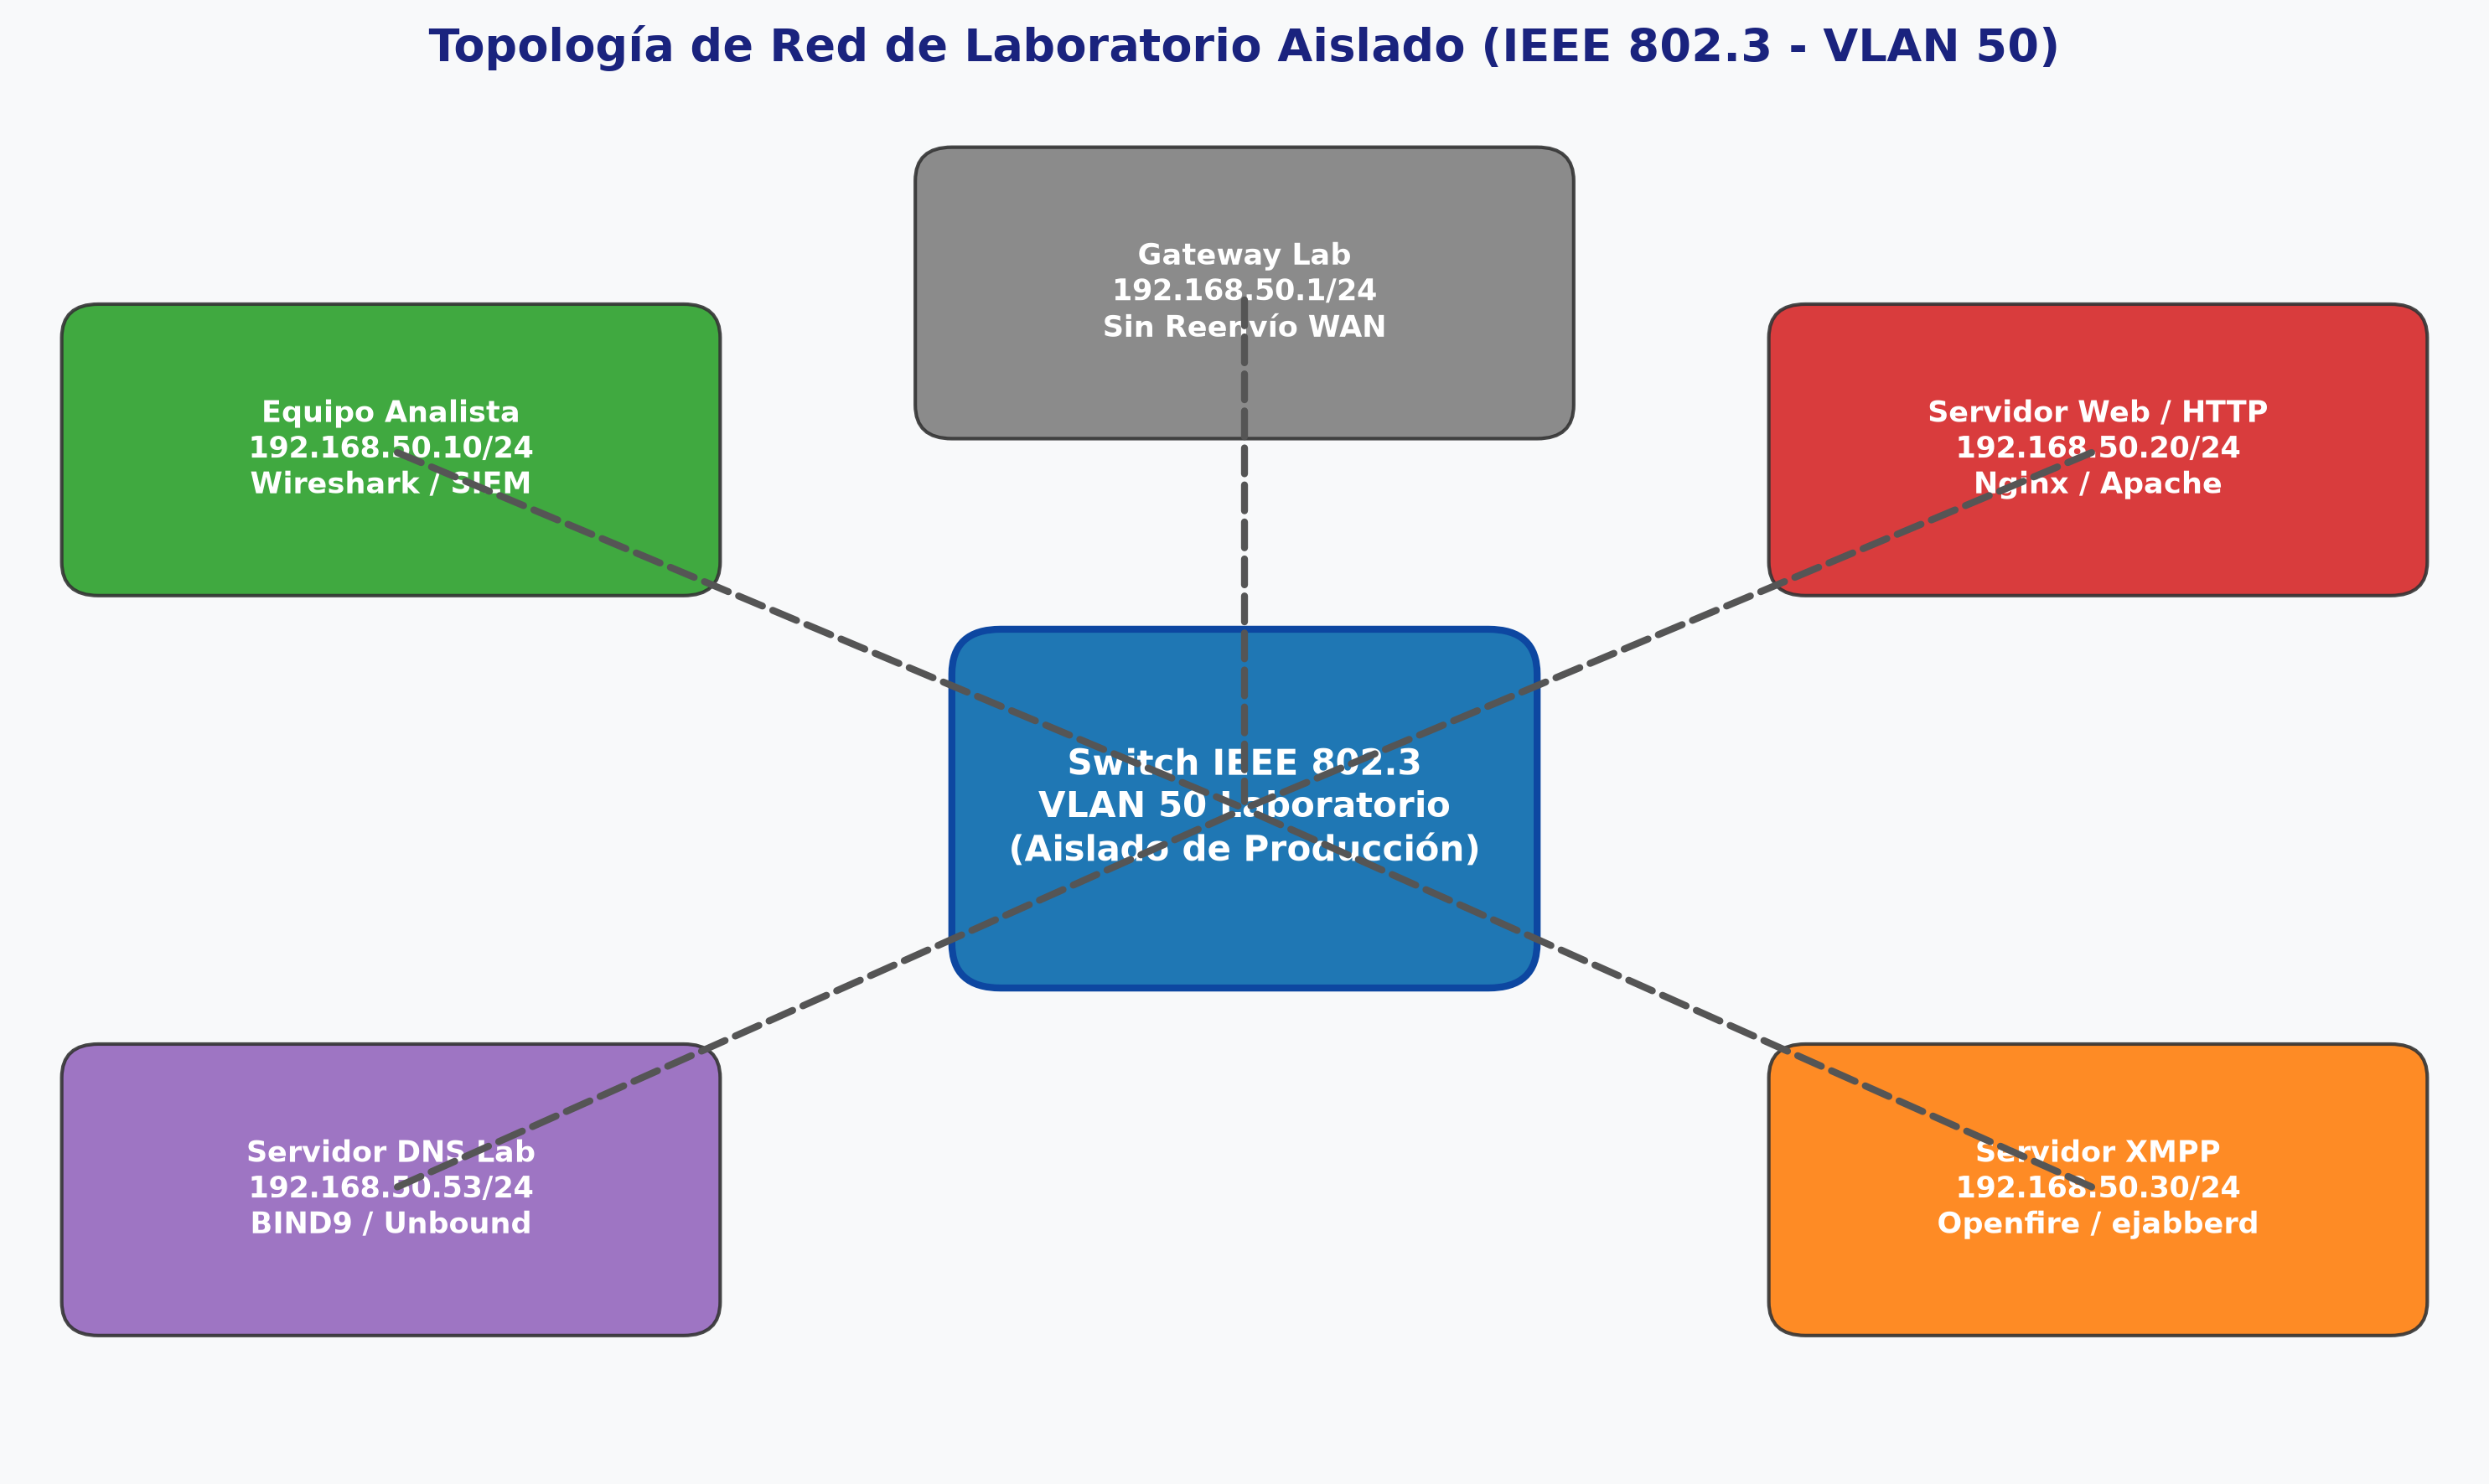
\includegraphics[width=0.28\textwidth]{./images/topologia_laboratorio.png}\\[1.2cm]

    {\huge \bfseries \textcolor{udazul}{INFORME TÉCNICO DE LABORATORIO}}\\[0.4cm]
    {\LARGE \bfseries GUÍA--TALLER No. 2}\\[0.5cm]
    {\Large \textbf{Mecanismos de Seguridad para Redes IEEE 802.3 con Servidores TCP/IP y Sistema de Rastreo Inteligente con IA}}\\[1.8cm]

    \begin{minipage}{0.48\textwidth}
        \begin{flushleft} \large
            \textbf{Estudiantes Investigadores:}\\
            Grupo de Investigación y Ciberseguridad\\
            Ingeniería de Sistemas - Redes\\
            Universidad Distrital FJDC
        \end{flushleft}
    \end{minipage}
    \begin{minipage}{0.48\textwidth}
        \begin{flushright} \large
            \textbf{Docente Titular:}\\
            Ing. Octavio José Salcedo Parra\\
            \textit{Fundamentos de Redes de Comunicaciones}\\
            \textit{Mecanismos de Seguridad Informática}
        \end{flushright}
    \end{minipage}

    \vfill
    {\large Bogotá D.C., Colombia\\Noviembre 14 / 2026}
\end{titlepage}

\newpage
\tableofcontents
\newpage

% ==============================================================================
% SECCIÓN 1: RESUMEN EJECUTIVO Y ALCANCE
% ==============================================================================
\section{Resumen Ejecutivo y Alcance del Laboratorio}

El presente informe consolida el desarrollo integral de la \textbf{Guía--Taller No. 2}, orientada a la identificación, análisis forense, mitigación y contención de riesgos sobre la disponibilidad, confidencialidad e integridad en arquitecturas de red de área local Ethernet \textbf{IEEE 802.3} que transportan protocolos de la pila \textbf{TCP/IP} (IPv4/IPv6).

El laboratorio se estructura en dos componentes complementarios:
\begin{enumerate}
    \item \textbf{Parte I: Análisis Forense y Defensivo de 10 Casos Críticos de Red:} Evaluación exhaustiva de ataques de agotamiento de recursos (TCP SYN Flood), canales encubiertos y exfiltración (DNS e ICMP Tunneling), exposición de servicios obsoletos en texto claro (HTTP/FTP/Telnet), inyecciones de control (TCP Resets desincronizados), amplificación volumétrica UDP (DNS/NTP/SSDP), escaneo sigiloso y fingerprinting, culminando con la priorización y correlación multicapa asistida por Inteligencia Artificial (SIEM/ML) y la auditoría criptográfica de mensajería XMPP con TLS.
    \item \textbf{Parte II: Desarrollo de Sistema Inteligente de Rastreo Ético y Geofencing:} Diseño e implementación de una plataforma completa de software (Backend REST en FastAPI, Base de Datos SQLite, Frontend interactivo con mapas Leaflet.js, Bot interactivo de mensajería en Telegram y Motor de Machine Learning Cinemático) orientada a la localización consentida de terminales, delimitación de geocercas y detección heurística de anomalías espaciotemporales (anti-spoofing).
\end{enumerate}

\subsection{Diferenciación Epistemológica en la Investigación de Incidentes}
Conforme a los lineamientos pedagógicos del laboratorio, el equipo analista mantiene una rigurosa separación entre las fases de investigación técnica:
\begin{itemize}
    \item \textbf{Síntoma:} Manifestación fenomenológica superficial u operativa observable en el sistema (ej. degradación en el tiempo de respuesta del servidor web, latencia inusual en consultas DNS o reinicios esporádicos de conexión).
    \item \textbf{Indicador de Compromiso (IoC):} Evidencia objetiva y cuantificable recolectada en telemetría de red o bitácoras que sugiere una desviación anómala (ej. tasa de paquetes SYN sin ACK superior a 800 pps, subdominios DNS con longitud $> 50$ caracteres y entropía $> 4.2$ bits/char).
    \item \textbf{Hipótesis:} Formulación causal estructurada que busca explicar la correlación de síntomas e indicadores evaluando alternativas tanto maliciosas como benignas (ej. ¿Se trata de un ataque DoS distribuido o de una congestión legítima producida por un reintento masivo tras caída de enlace?).
    \item \textbf{Evidencia Confirmada:} Conclusión técnica demostrada mediante pruebas reproducibles, inspección de paquetes en profundidad (DPI), verificación de integridad criptográfica y descarte riguroso de hipótesis alternas.
\end{itemize}

\subsection{Topología del Laboratorio Aislado y Reglas de Trabajo}
La práctica se ejecutó en un entorno controlado y virtualizado, aislado de redes institucionales en producción y de Internet, empleando el esquema de direccionamiento privado clase C \texttt{192.168.50.0/24} (VLAN 50).

\begin{figure}[H]
    \centering
    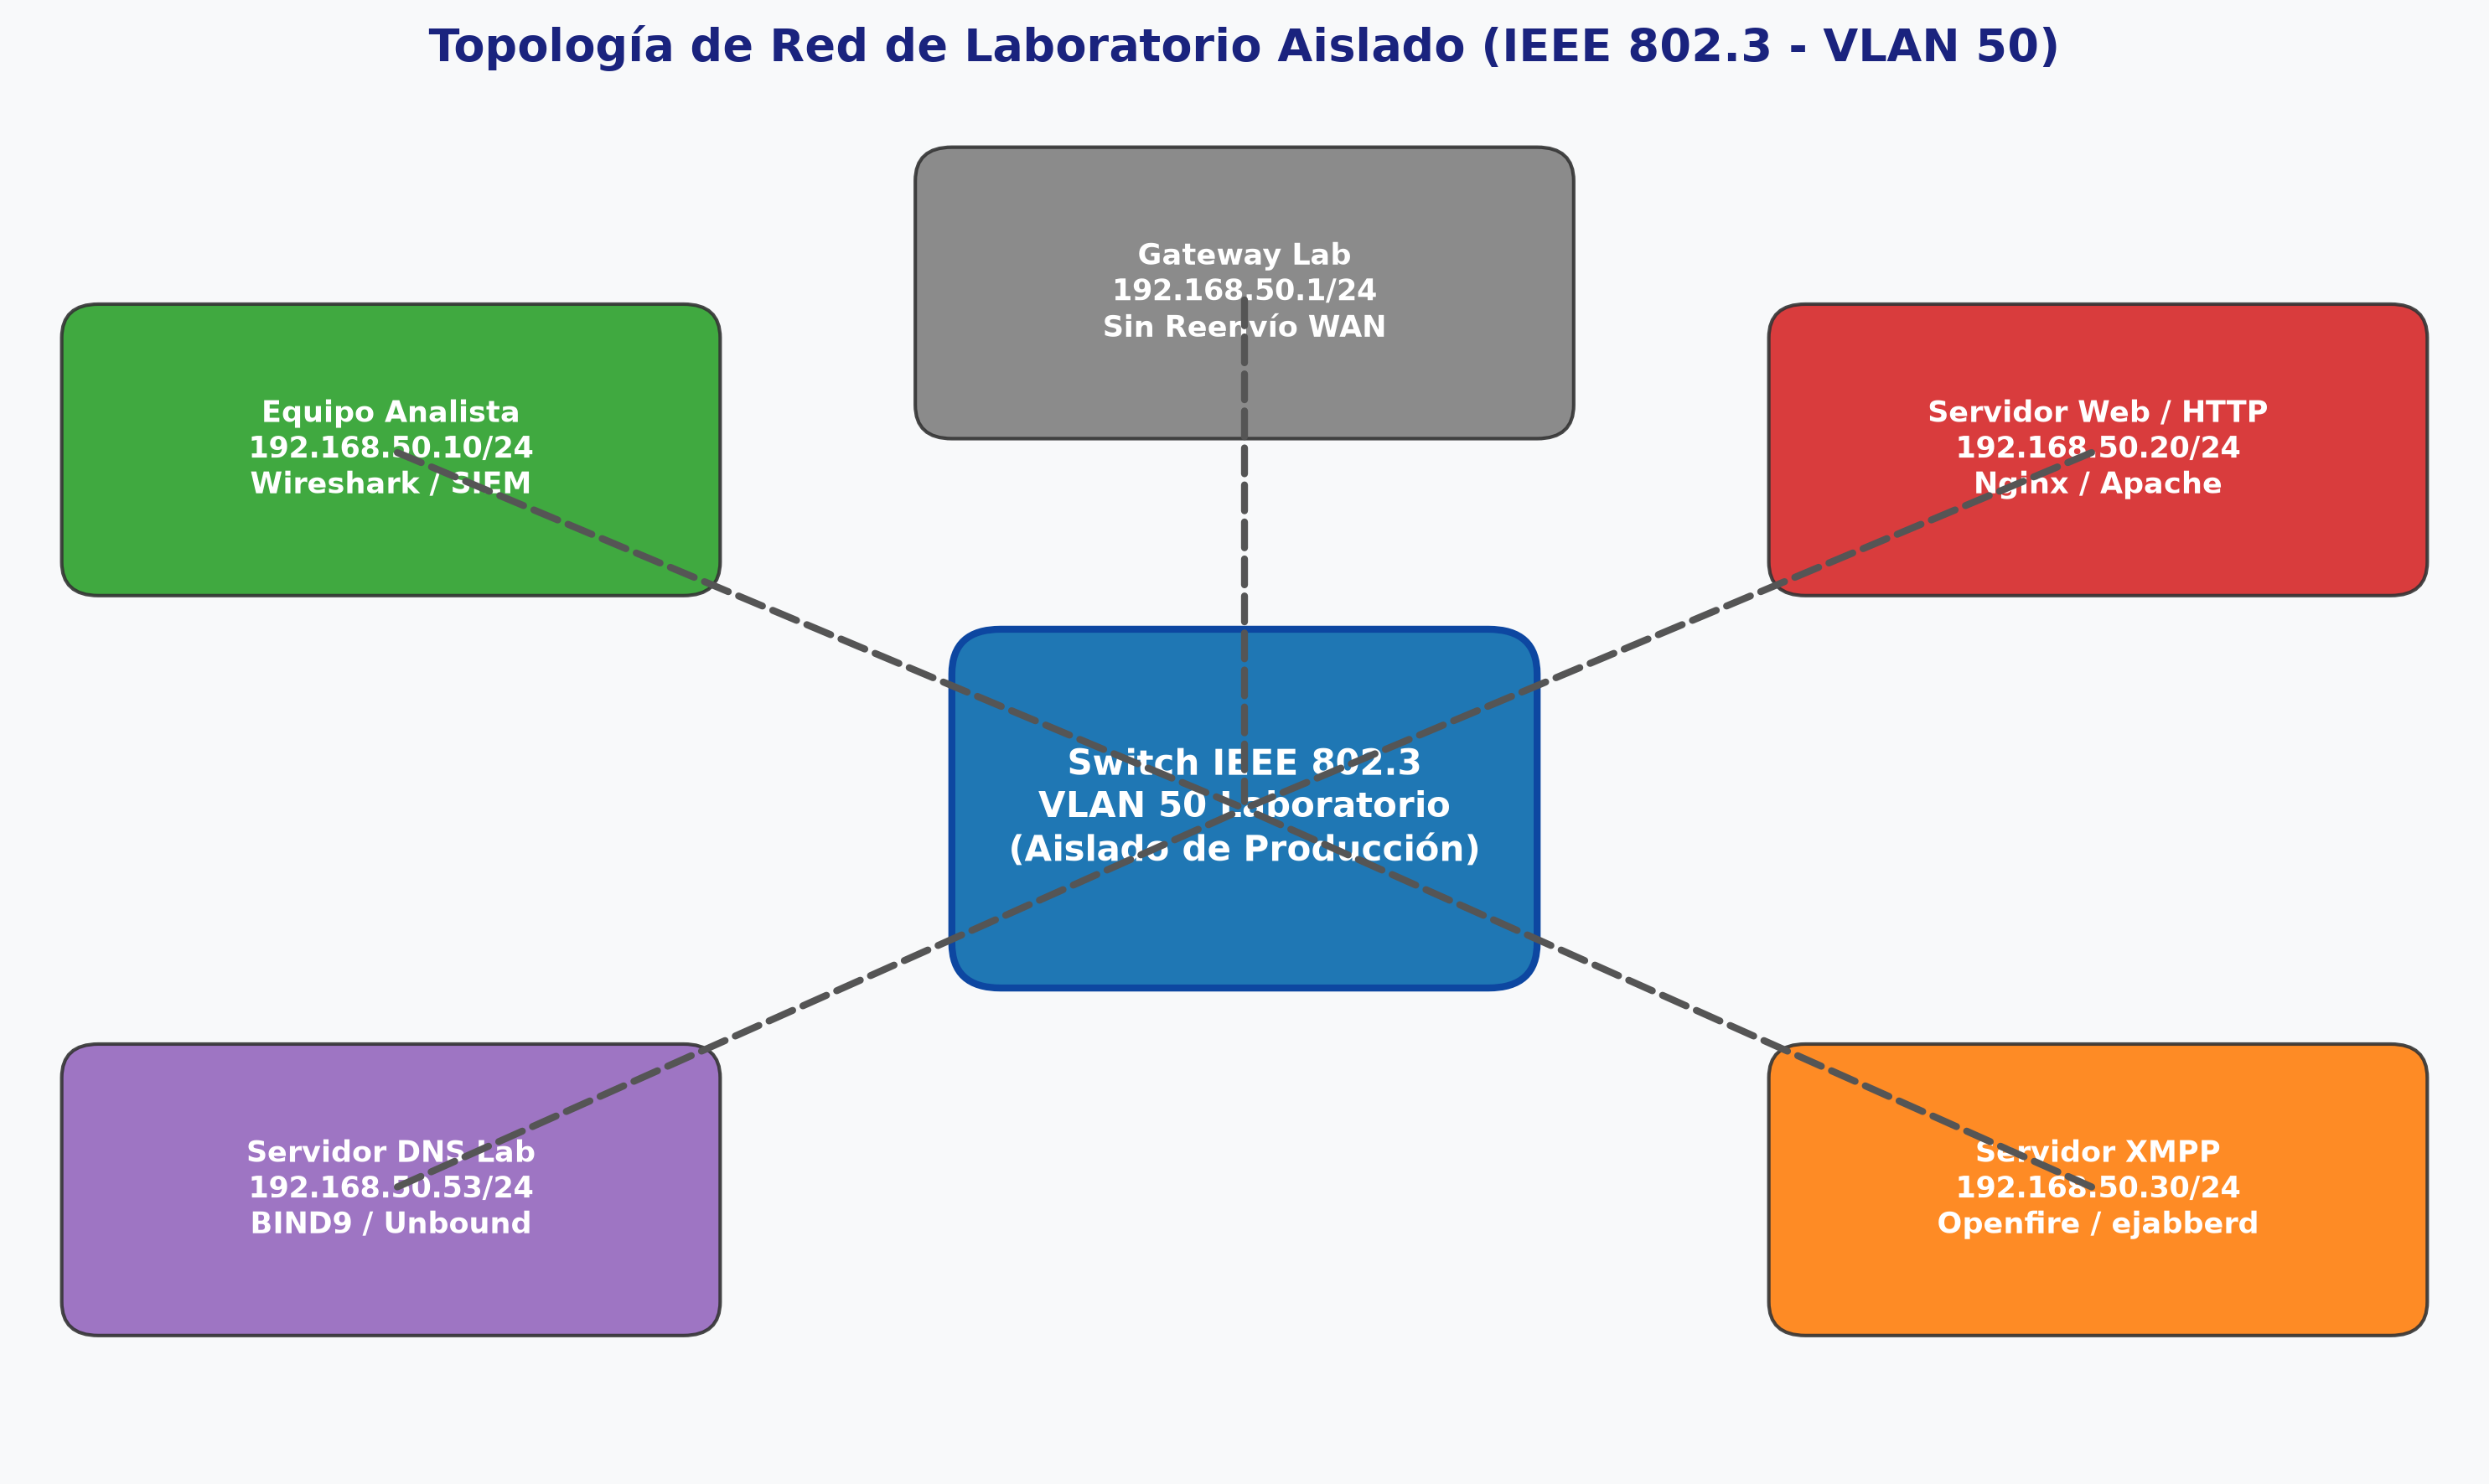
\includegraphics[width=0.88\textwidth]{./images/topologia_laboratorio.png}
    \caption{Topología del Laboratorio Académico Aislado (IEEE 802.3 - VLAN 50).}
    \label{fig:topologia}
\end{figure}

\begin{table}[H]
    \centering
    \small
    \begin{tabular}{@{}llll@{}}
        \toprule
        \textbf{Elemento} & \textbf{Dirección IP / Función} & \textbf{Software / Rol} & \textbf{Recomendación Aplicada} \\
        \midrule
        Switch Ethernet & VLAN 50 Laboratorio & Switch Virtual IEEE 802.3 & Segmentación total; sin puente a WAN \\
        Equipo Analista & 192.168.50.10/24 & Wireshark, Python, SIEM & Inspección pasiva, generación controlada \\
        Servidor Web & 192.168.50.20/24 & Apache 2.4 / Nginx / ProFTPD & Servidor objetivo de pruebas benignas \\
        Servidor DNS & 192.168.50.53/24 & Resolver Unbound / BIND9 & Resolución local exclusiva sin recursión WAN \\
        Servidor XMPP & 192.168.50.30/24 & Openfire 4.7.1 / TLS & Mensajería instantánea aislada \\
        Gateway Lab & 192.168.50.1/24 & Router Linux con iptables & Filtrado perimetral estricto; bloqueo de WAN \\
        \bottomrule
    \end{tabular}
    \caption{Distribución de Nodos y Servicios en la Red de Laboratorio.}
\end{table}

\subsection{Cadena de Custodia Criptográfica de Evidencias (SHA-256)}
Para garantizar la inalterabilidad y reproducibilidad de las capturas de tráfico sintético analizadas, cada archivo \texttt{.pcap} generado cuenta con su huella digital criptográfica SHA-256 registrada antes de iniciar el análisis forense sobre copias de trabajo:

\begin{table}[H]
    \centering
    \footnotesize
    \begin{tabular}{@{}llrl@{}}
        \toprule
        \textbf{Caso / Archivo PCAP} & \textbf{Tamaño} & \textbf{Hash Criptográfico SHA-256} & \textbf{Estado} \\
        \midrule
        \texttt{caso1\_syn\_flood.pcap} & 16,128 B & \texttt{8d0e5fda4547e9cad8608aaff3412664d8a4d8e90fbb102fa4542ca2e3a070ea} & Verificado \\
        \texttt{caso2\_dns\_tunneling.pcap} & 2,594 B & \texttt{bdddff6608a856ed593186747f5e36ed5f69f2d2457b1ad8ee88f13a112ec6f0} & Verificado \\
        \texttt{caso5\_tcp\_resets.pcap} & 469 B & \texttt{083f4940a9a73111fe20f58628fa7febdf971f6ec8a0a88b6f9240e858eef082} & Verificado \\
        \texttt{caso6\_udp\_amplification.pcap} & 14,224 B & \texttt{205127ca90fff94b2ee7f3833a4595c68581fe2abb0232c3fbcf70af222db1bd} & Verificado \\
        \texttt{caso7\_icmp\_tunnel.pcap} & 6,234 B & \texttt{e0512a71b74db26dabcf514d786c31ff825973535435cc0985bf43c78cf2ae98} & Verificado \\
        \texttt{caso8\_port\_scan.pcap} & 2,194 B & \texttt{4e8907bad8c3012326e6c8a9746d5f65f788225b6a1989d6ea404c8d7ac31545} & Verificado \\
        \bottomrule
    \end{tabular}
    \caption{Registro de Integridad Criptográfica de Evidencias Digitales.}
\end{table}

\newpage
% ==============================================================================
% SECCIÓN 2: PARTE I - LOS 10 CASOS CRÍTICOS DE TRABAJO
% ==============================================================================
\section{Parte I: Desarrollo de Casos Críticos de Seguridad de Red}

% ------------------------------------------------------------------------------
% CASO 1
% ------------------------------------------------------------------------------
\subsection{Caso 1: TCP SYN Flood: Indisponibilidad y Agotamiento de Conexiones}

\paragraph{Situación:} El servidor web (\texttt{192.168.50.20}) experimenta indisponibilidad intermitente; los clientes legítimos sufren retardos severos o incapacidad de establecer el saludo de tres vías (three-way handshake).

\paragraph{Procedimiento y Observación:}
\begin{enumerate}
    \item Se capturó tráfico en la interfaz de red del servidor y se correlacionó con comandos del sistema operativo.
    \item En Windows Server / PowerShell se ejecutó:
    \begin{lstlisting}[language=bash]
    netstat -ano -p tcp | Select-String "192.168.50.20:80"
    Get-NetTCPConnection -State SynReceived
    \end{lstlisting}
    \item Se observaron cientos de conexiones bloqueadas en estado \texttt{SYN\_RECEIVED} asignadas al proceso \texttt{nginx.exe} (PID 4216).
    \item En la captura de tráfico se constató un desbalance crítico: más de 850 paquetes SYN por segundo frente a una ausencia total de paquetes ACK correspondientes desde las direcciones IP de origen.
\end{enumerate}

\begin{figure}[H]
    \centering
    \begin{subfigure}[b]{0.58\textwidth}
        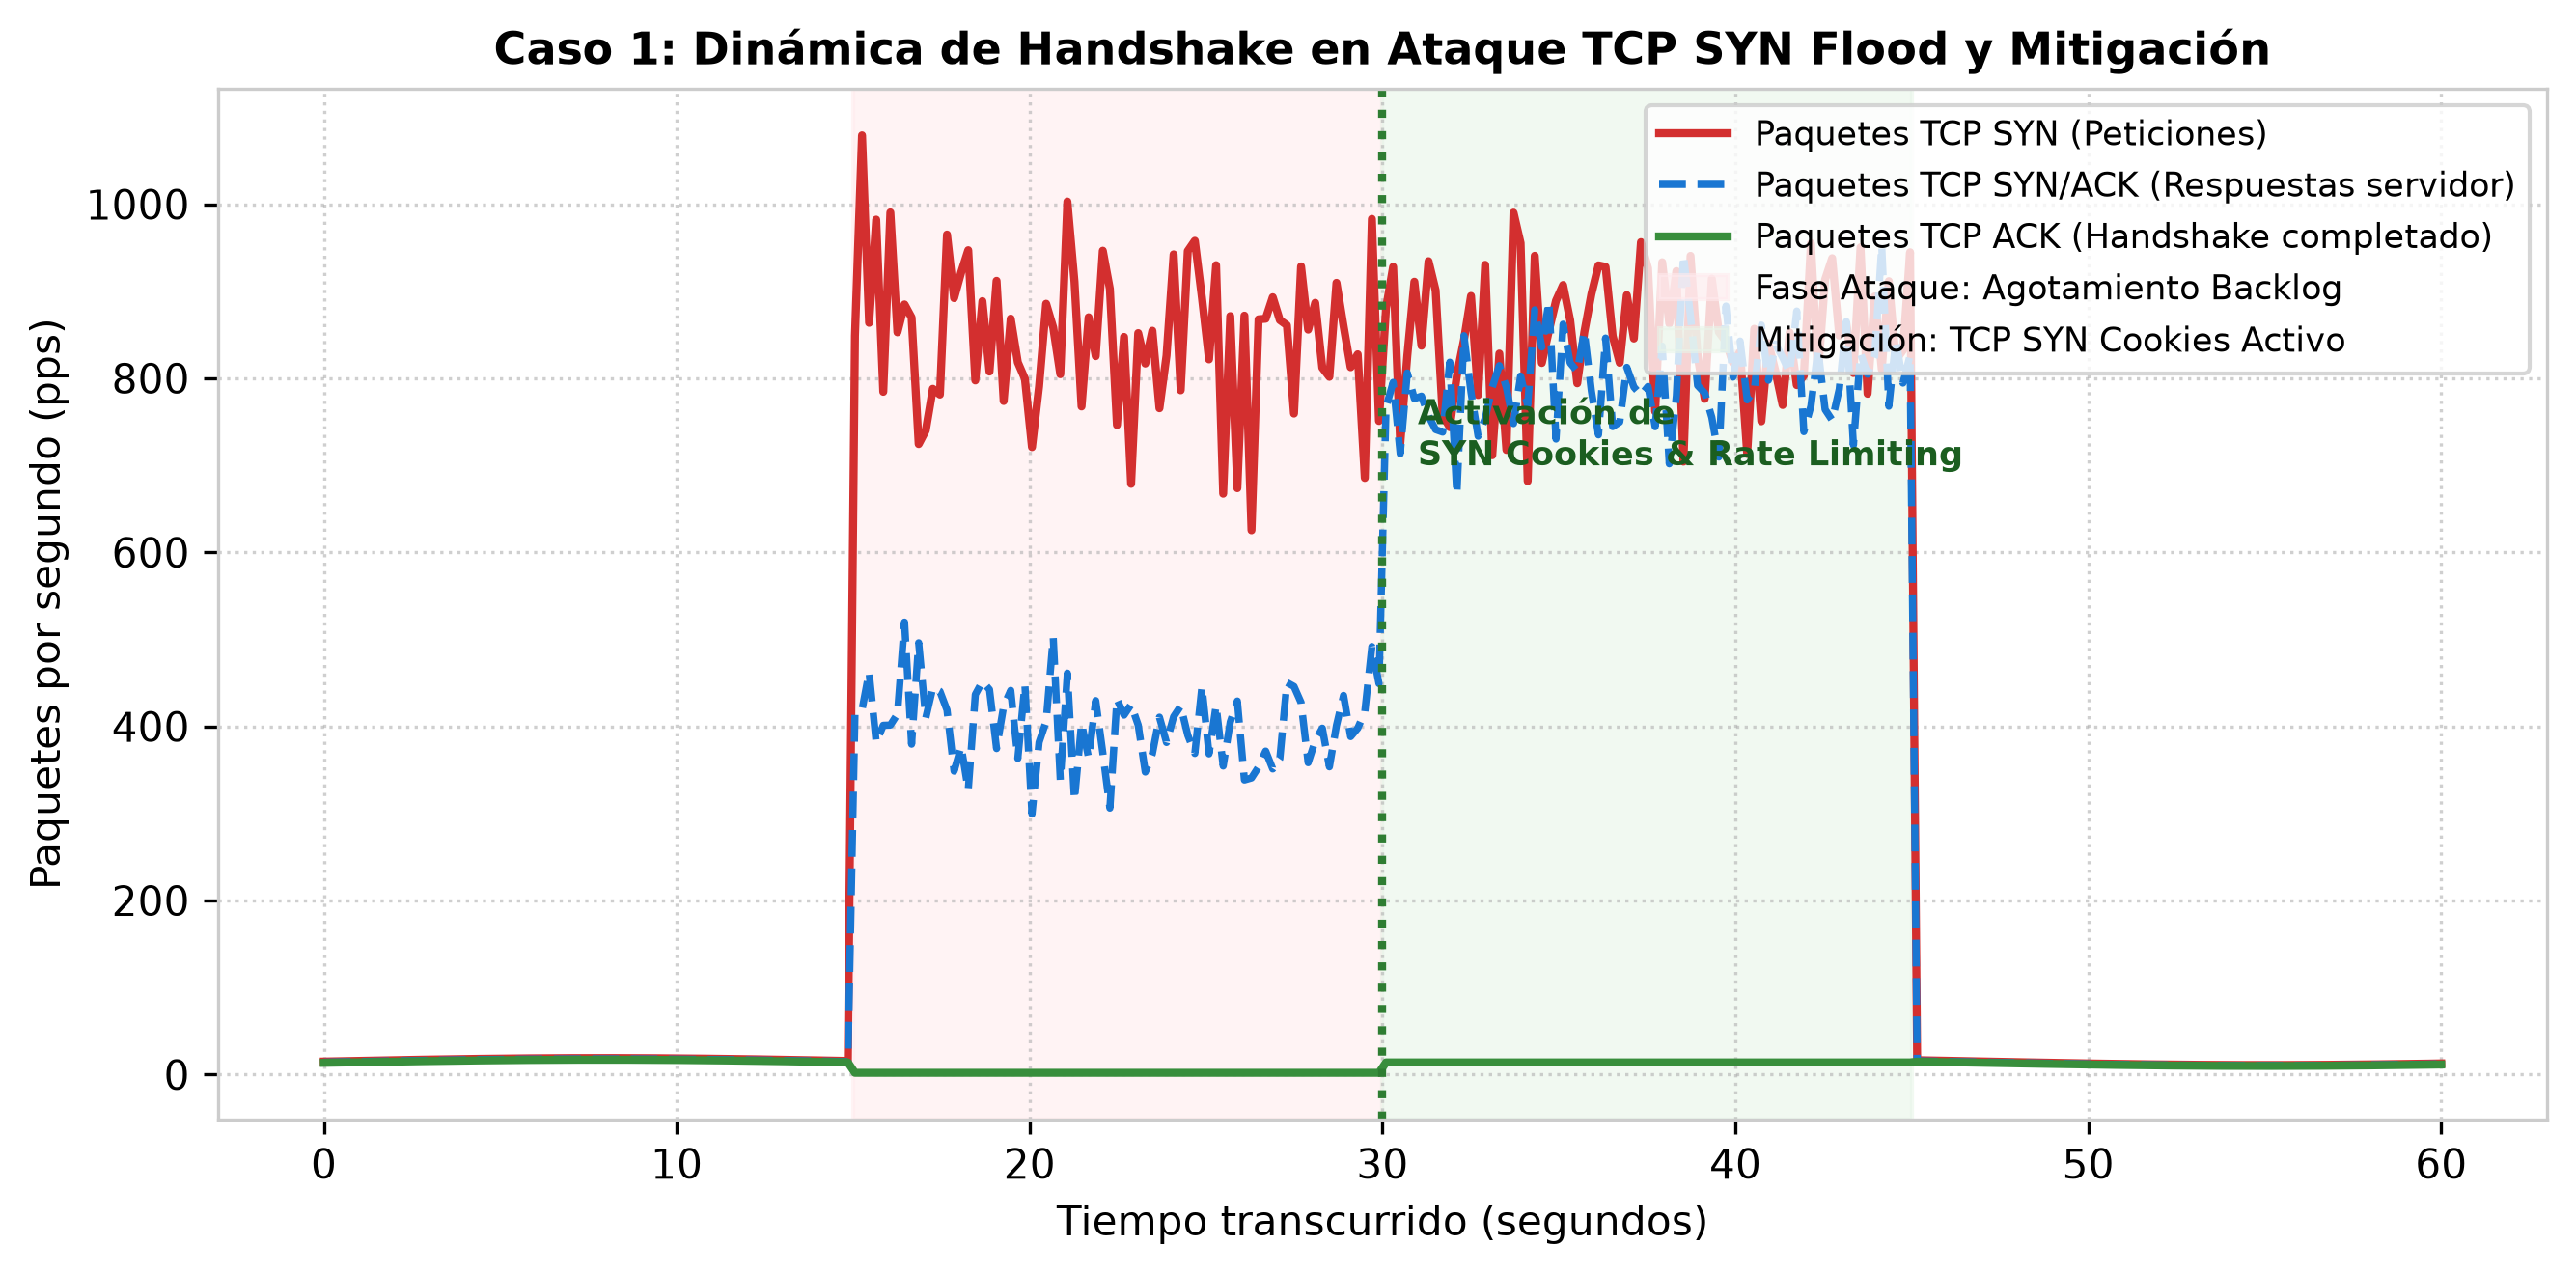
\includegraphics[width=\textwidth]{./images/caso1_synflood_rates.png}
        \caption{Dinámica temporal de tasas SYN, SYN-ACK y ACK.}
    \end{subfigure}
    \hfill
    \begin{subfigure}[b]{0.40\textwidth}
        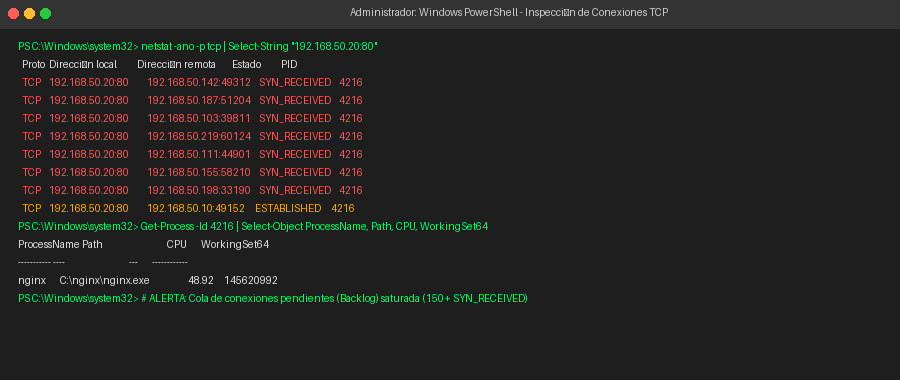
\includegraphics[width=\textwidth]{./images/caso1_netstat_terminal.png}
        \caption{Inspección de conexiones en terminal PowerShell.}
    \end{subfigure}
    \caption{Evidencia de Agotamiento de Backlog por TCP SYN Flood y Mitigación.}
    \label{fig:caso1_evidencia}
\end{figure}

\paragraph{Mitigación y Controles:}
\begin{itemize}
    \item \textbf{Control Preventivo:} Habilitación de \textit{TCP SYN Cookies} en la pila del núcleo del sistema operativo (\texttt{net.ipv4.tcp\_syncookies = 1} en Linux o activación de protección SYN en Windows Defender Firewall mediante el registro \texttt{SynAttackProtect = 2}).
    \item \textbf{Control Detectivo:} Monitorización en tiempo real de la longitud de la cola de conexiones semi-abiertas (\texttt{ListenBacklog}) mediante alertas SNMP y reglas Suricata.
    \item \textbf{Control Correctivo:} Aplicación de límite de tasa (\textit{rate limiting}) en el gateway de laboratorio:
    \begin{lstlisting}[language=bash]
    iptables -A INPUT -p tcp --syn --dport 80 -m connlimit --connlimit-above 30 --connlimit-mask 32 -j DROP
    iptables -A INPUT -p tcp --syn --dport 80 -m hashlimit --hashlimit-name syn_limit --hashlimit-above 50/sec --hashlimit-burst 100 --hashlimit-mode srcip -j DROP
    \end{lstlisting}
\end{itemize}

\paragraph{Respuestas a Preguntas de Análisis:}
\begin{enumerate}
    \item \textbf{¿Qué recursos mantiene el servidor durante el handshake TCP?} Durante el estado semi-abierto (\texttt{SYN\_RECEIVED}), el kernel asigna una estructura de datos en memoria denominada Bloque de Control de Transmisión (TCB - \textit{Transmission Control Block} o \texttt{struct inet\_request\_sock}). Dicha estructura reserva memoria RAM para almacenar los números de secuencia iniciales (ISN), opciones TCP negociadas (MSS, Window Scale, SACK Permitted), direcciones IP y puertos, punteros a temporizadores de retransmisión exponencial para el SYN-ACK y entradas en la tabla hash de conexiones pendientes (\textit{SYN Backlog Queue}). Un ataque masivo satura esta cola finita, provocando el descarte silencioso de nuevas peticiones legítimas.
    \item \textbf{¿Qué falsos positivos pueden producir picos legítimos?} Los picos súbitos de paquetes SYN pueden originarse legítimamente por: (a) El \textit{Efecto Slashdot} o \textit{Flash Crowd}, derivado de noticias de última hora o aperturas de matrículas universitarias; (b) Recuperación tras fallos de conectividad o reinicio de un enlace troncal, donde cientos de clientes reconectan de manera sincronizada; (c) Desconexión y reintento de clientes móviles bajo mala cobertura celular con alta pérdida de paquetes; y (d) Balancers de carga o proxies reversos configurados con Keep-Alive insuficiente.
\end{enumerate}

\begin{hallazgobox}{Ficha de Registro de Hallazgo -- Caso 1}
    \textbf{Identificador:} CASO-01-SYN-001 \hfill \textbf{Analista:} Equipo Ciberseguridad UD\\
    \textbf{Fecha / Hora:} 2026-11-03 10:02:12 UTC-5 \hfill \textbf{Sincronización:} NTP Local Sincronizado\\
    \textbf{Origen / Destino:} IPs Múltiples (192.168.50.100--240) $\rightarrow$ 192.168.50.20:80 (TCP)\\
    \textbf{Observación Fáctica:} Se reciben 850 paquetes SYN/s continuos. El servidor responde SYN-ACK pero no ingresa ningún paquete ACK final. El backlog del puerto 80 alcanza el 100\% de ocupación.\\
    \textbf{Hipótesis y Alternativas:} Hipótesis Principal: Ataque DoS por inundación SYN con IPs de origen falsificadas (spoofed). Hipótesis Alternativa Benigna descartada: Caída masiva de red de clientes (no se aprecian retransmisiones legítimas sino flujos efímeros).\\
    \textbf{Validación Técnica:} Análisis de PCAP (\texttt{tcp.flags.syn==1 and tcp.flags.ack==0}), salida de \texttt{netstat -ano} con 150+ conexiones en \texttt{SYN\_RECEIVED}.\\
    \textbf{Severidad:} CRÍTICA (Impacto Alto en Disponibilidad, Probabilidad Alta).\\
    \textbf{Acción Correctiva:} Activación de TCP SYN Cookies y regla \texttt{hashlimit} en firewall perimetral.\\
    \textbf{Integridad de Evidencia:} \texttt{caso1\_syn\_flood.pcap} (16,128 B) | SHA-256: \texttt{8d0e5fda4547e9cad8608aaff3412664d8a4d8e90fbb102fa4542ca2e3a070ea}
\end{hallazgobox}

\newpage
% ------------------------------------------------------------------------------
% CASO 2
% ------------------------------------------------------------------------------
\subsection{Caso 2: DNS Tunneling: Salida Encubierta mediante UDP/53}

\paragraph{Situación:} Se detecta tráfico anómalo sobre el protocolo DNS (\texttt{UDP/53}) proveniente del equipo analista hacia el resolver del laboratorio con consultas a nombres de dominio de longitud inusual.

\paragraph{Procedimiento y Observación:}
\begin{enumerate}
    \item Se filtró el tráfico en Wireshark con \texttt{udp.port == 53} y \texttt{dns}.
    \item Se calcularon métricas de longitud de subdominios y Entropía de la Información de Shannon sobre las etiquetas de consulta:
    \begin{equation}
        H(X) = -\sum_{i=1}^{n} P(x_i) \log_2 P(x_i)
    \end{equation}
    \item Se detectaron consultas continuas del tipo TXT dirigidas a dominios con cadenas en Base64/Hexadecimal (ej. \texttt{4a66396b6c73839a.c2-exfil.lab}), cuyas respuestas devuelven fragmentos de comandos cifrados.
\end{enumerate}

\begin{figure}[H]
    \centering
    \begin{subfigure}[b]{0.52\textwidth}
        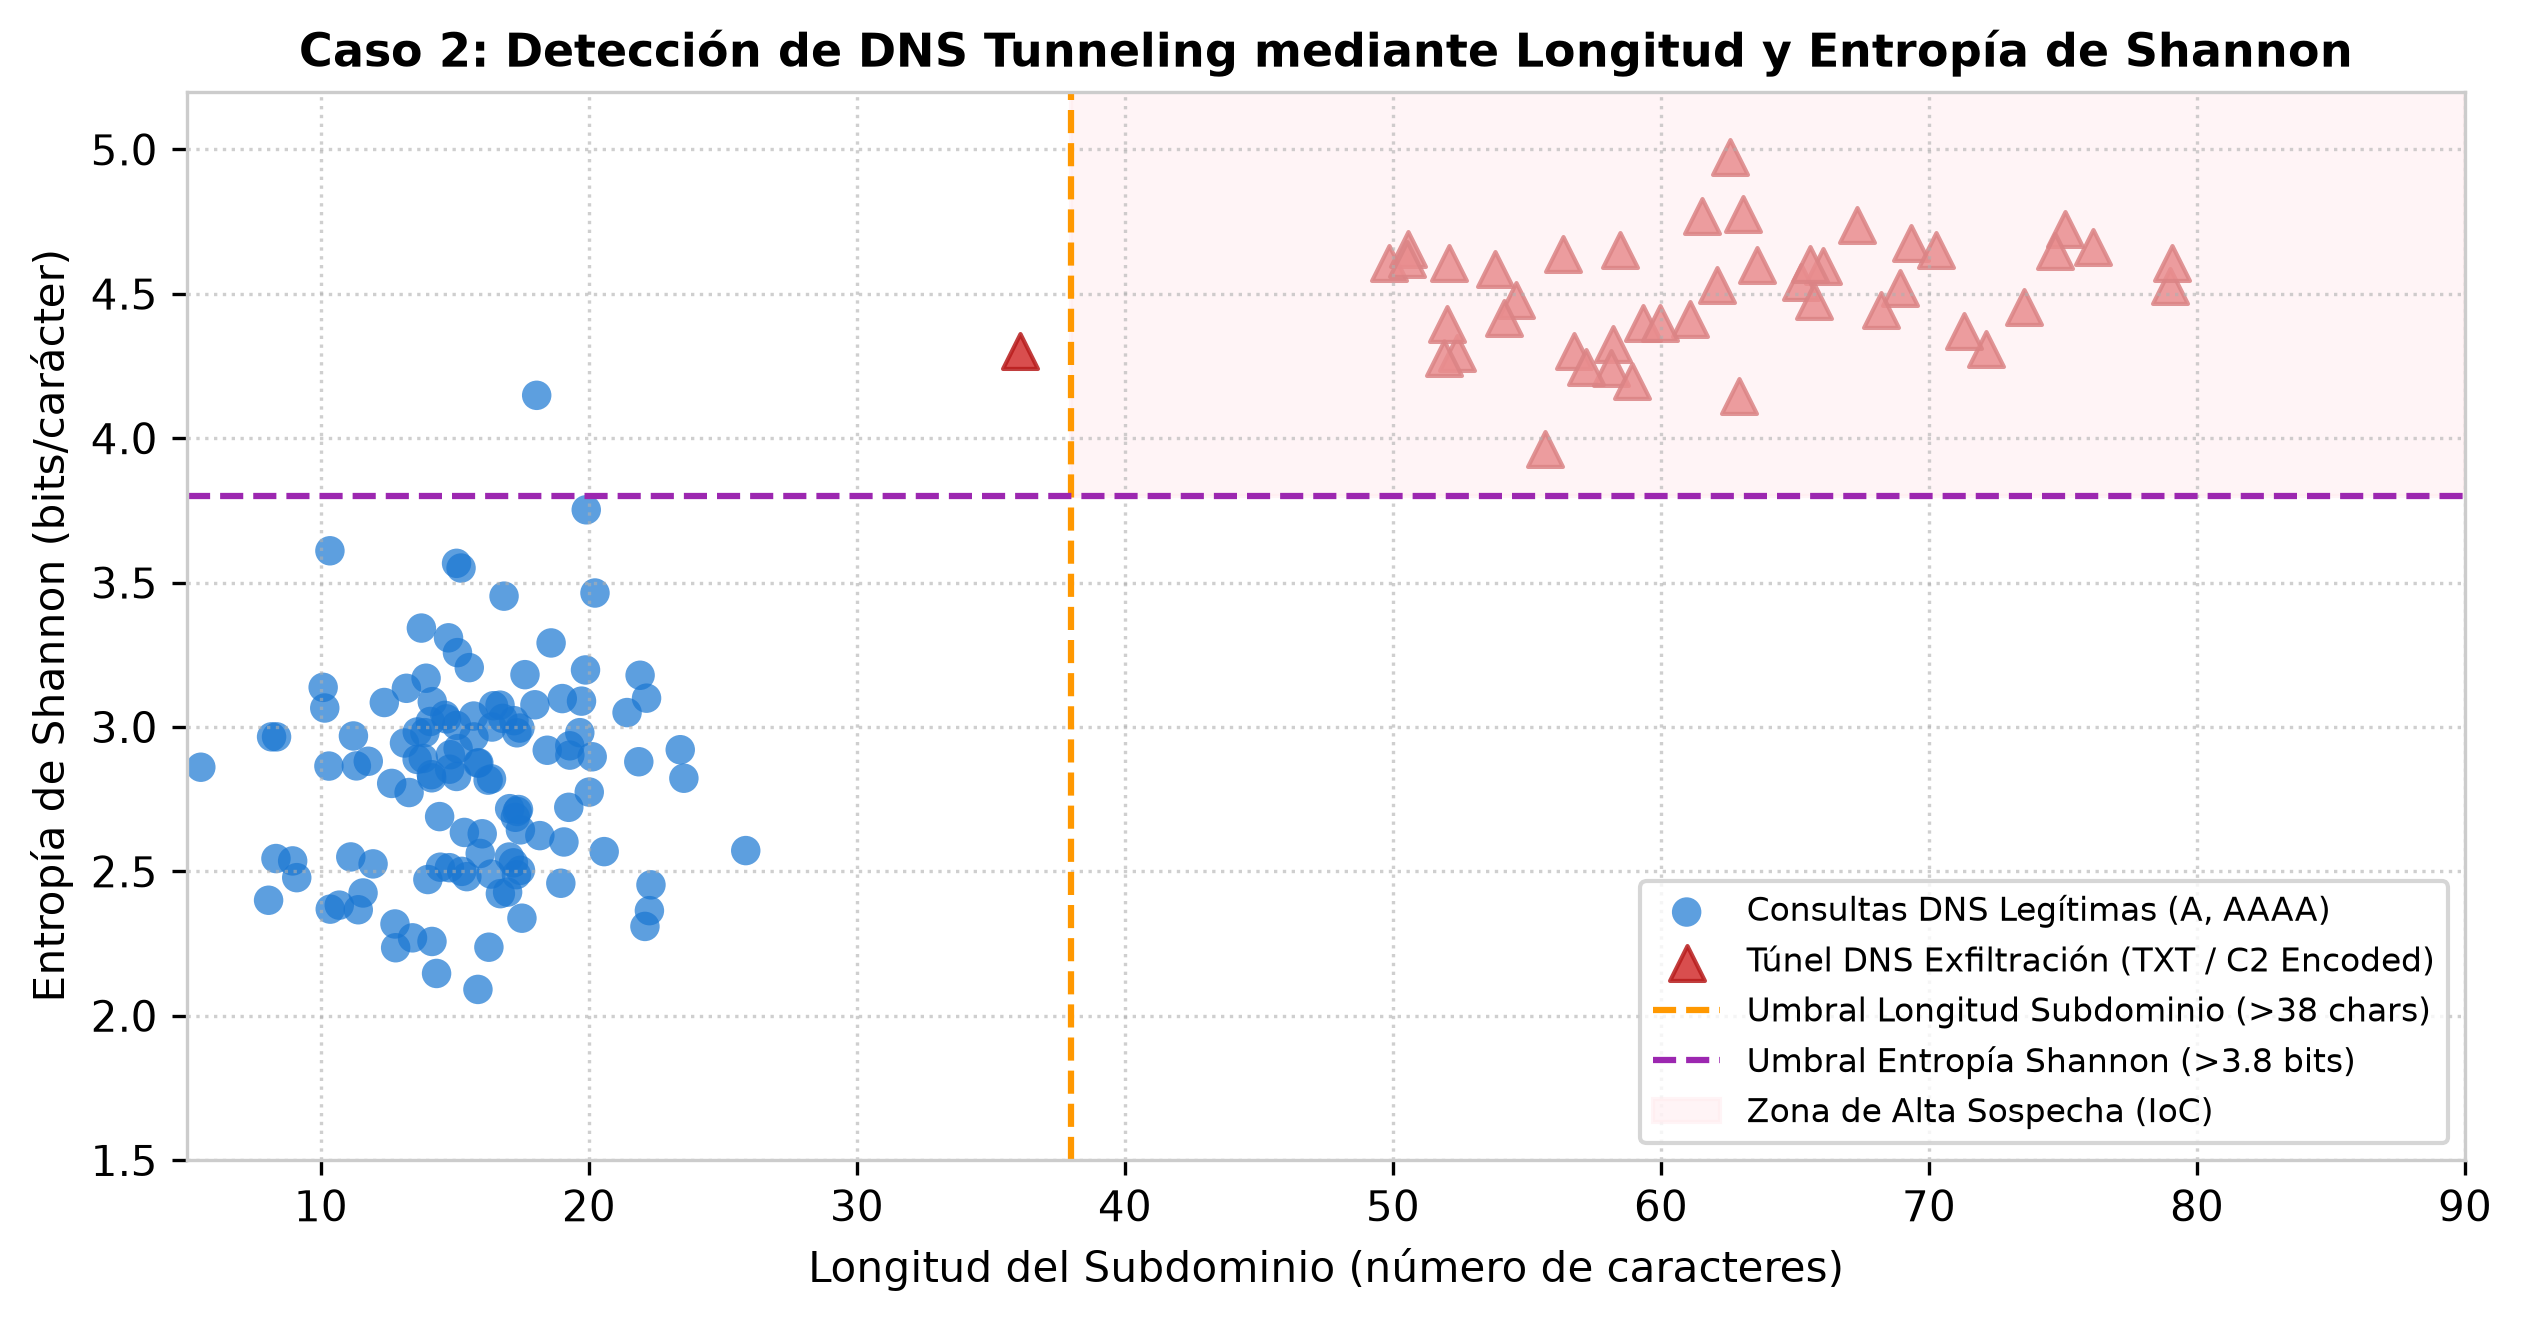
\includegraphics[width=\textwidth]{./images/caso2_dnstunnel_entropy.png}
        \caption{Dispersión de Longitud vs. Entropía de Shannon.}
    \end{subfigure}
    \hfill
    \begin{subfigure}[b]{0.46\textwidth}
        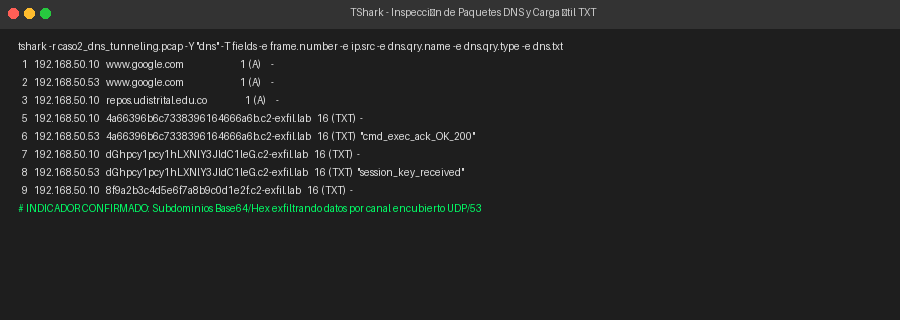
\includegraphics[width=\textwidth]{./images/caso2_wireshark_dns.png}
        \caption{Inspección de tramas DNS con TShark.}
    \end{subfigure}
    \caption{Detección Forense de Canal Encubierto por DNS Tunneling.}
    \label{fig:caso2_evidencia}
\end{figure}

\paragraph{Mitigación y Controles:}
\begin{itemize}
    \item \textbf{Control Preventivo:} Prohibición en el firewall perimetral de cualquier tráfico saliente hacia UDP/TCP puerto 53 que no provenga del servidor resolver corporativo (\texttt{192.168.50.53}).
    \item \textbf{Control Detectivo:} Implementación de zonas de políticas de respuesta (DNS RPZ) y reglas en Suricata inspeccionando longitud de FQDN y tipos de registro anómalos:
    \begin{lstlisting}[language=bash]
    alert dns $HOME_NET any -> any 53 (msg:"DNS Tunneling - Longitud o Entropia Anomala"; dns.query; content:".c2-exfil"; nocase; pcre:"/^[a-zA-Z0-9]{35,}\./"; sid:1000021; rev:1;)
    \end{lstlisting}
    \item \textbf{Control Correctivo:} Aislamiento del endpoint origen para escaneo de malware y revocación de credenciales.
\end{itemize}

\paragraph{Respuestas a Preguntas de Análisis:}
\begin{enumerate}
    \item \textbf{¿Por qué el carácter sin conexión de UDP no significa que todo DNS sea malicioso?} El protocolo DNS adoptó UDP por motivos de eficiencia, ligereza y escalabilidad: la gran mayoría de las resoluciones de nombres consisten en un único par petición-respuesta que se resuelve en milisegundos sin la sobrecarga computacional y de latencia del handshake TCP. La ausencia de estado inherente a UDP es una decisión de arquitectura de Internet para optimizar el rendimiento masivo, no una señal intrínseca de intencionalidad hostil.
    \item \textbf{¿Qué atributos ayudan a distinguir una anomalía?} Se destacan seis características determinantes: (1) \textit{Entropía de Shannon elevada} ($>3.8$ bits/carácter) debida a codificación Base32/Base64/Hex; (2) \textit{Longitud extrema de etiquetas} (cercanas al límite RFC de 63 bytes por etiqueta o 255 bytes por FQDN); (3) \textit{Alta proporción de registros inusuales} (predominio de TXT, NULL o CNAME frente a consultas estándar A/AAAA); (4) \textit{Frecuencia y volumen elevado} de consultas a un mismo dominio de segundo nivel (\texttt{SLD}) con subdominios únicos efímeros; (5) \textit{Tiempos de vida (TTL) nulos o ultra-bajos} (0 a 5 segundos) para evitar el almacenamiento en caché intermedio; y (6) \textit{Asimetría de datos} en cargas útiles.
\end{enumerate}

\begin{hallazgobox}{Ficha de Registro de Hallazgo -- Caso 2}
    \textbf{Identificador:} CASO-02-DNS-002 \hfill \textbf{Analista:} Equipo Ciberseguridad UD\\
    \textbf{Fecha / Hora:} 2026-11-03 10:02:13 UTC-5 \hfill \textbf{Sincronización:} NTP Local Sincronizado\\
    \textbf{Origen / Destino:} 192.168.50.10:54120 $\rightarrow$ 192.168.50.53:53 (UDP)\\
    \textbf{Observación Fáctica:} Peticiones DNS continuas tipo TXT con subdominios de más de 48 caracteres alfanuméricos con entropía superior a 4.4 bits. Servidor retorna cargas útiles con texto de comandos.\\
    \textbf{Hipótesis y Alternativas:} Hipótesis Principal: Canal encubierto de comando y control (C2) y exfiltración de datos mediante DNS Tunneling. Hipótesis Alternativa Benigna evaluada: Actualización de antivirus o telemetría CDN (Descartada: el dominio objetivo \texttt{c2-exfil.lab} carece de firma de fabricante y no está en listas blancas corporativas).\\
    \textbf{Validación Técnica:} Análisis con TShark y script de entropía sobre \texttt{caso2\_dns\_tunneling.pcap}.\\
    \textbf{Severidad:} ALTA (Riesgo inminente de fuga de datos e infiltración persistente).\\
    \textbf{Acción Correctiva:} Bloqueo de consultas a dominios no categorizados y aislamiento del host para análisis forense.\\
    \textbf{Integridad de Evidencia:} \texttt{caso2\_dns\_tunneling.pcap} (2,594 B) | SHA-256: \texttt{bdddff6608a856ed593186747f5e36ed5f69f2d2457b1ad8ee88f13a112ec6f0}
\end{hallazgobox}

\newpage
% ------------------------------------------------------------------------------
% CASO 3
% ------------------------------------------------------------------------------
\subsection{Caso 3: Exposición de Servicios HTTP, FTP y Otros Servicios Heredados}

\paragraph{Situación:} Auditoría inicial sobre el servidor de laboratorio (\texttt{192.168.50.20}) para inventariar puertos abiertos, versiones y evaluar la presencia de servicios inseguros o sin soporte.

\paragraph{Procedimiento y Observación:}
\begin{enumerate}
    \item Se ejecutó un sondeo de versiones y scripts NSE con Nmap:
    \begin{lstlisting}[language=bash]
    nmap -sV -sC -Pn -p- 192.168.50.20
    \end{lstlisting}
    \item Se identificaron múltiples servicios activos: FTP (\texttt{ProFTPD 1.3.5}), Telnet (\texttt{puerto 23/tcp}), HTTP en claro (\texttt{Apache 2.4.41}), SSH (\texttt{OpenSSH 8.9p1}) y XMPP (\texttt{Openfire 4.7.1}).
    \item Se constató que FTP permite inicio de sesión anónimo (\texttt{anonymous:anonymous}) y corresponde a una versión vulnerable a ejecución remota de comandos no autenticada (CVE-2015-3306 - módulo \texttt{mod\_copy}).
    \item El servicio Telnet transmite credenciales y comandos en texto plano sin cifrado de transporte.
\end{enumerate}

\begin{figure}[H]
    \centering
    \begin{subfigure}[b]{0.50\textwidth}
        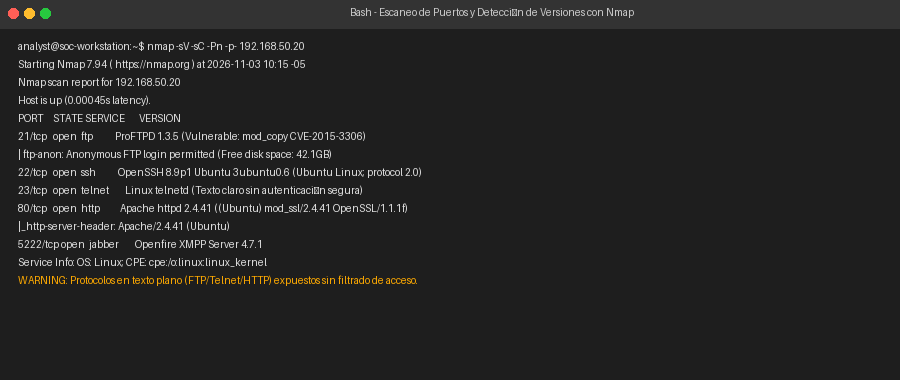
\includegraphics[width=\textwidth]{./images/caso3_nmap_services.png}
        \caption{Captura del escaneo de puertos y versiones Nmap.}
    \end{subfigure}
    \hfill
    \begin{subfigure}[b]{0.48\textwidth}
        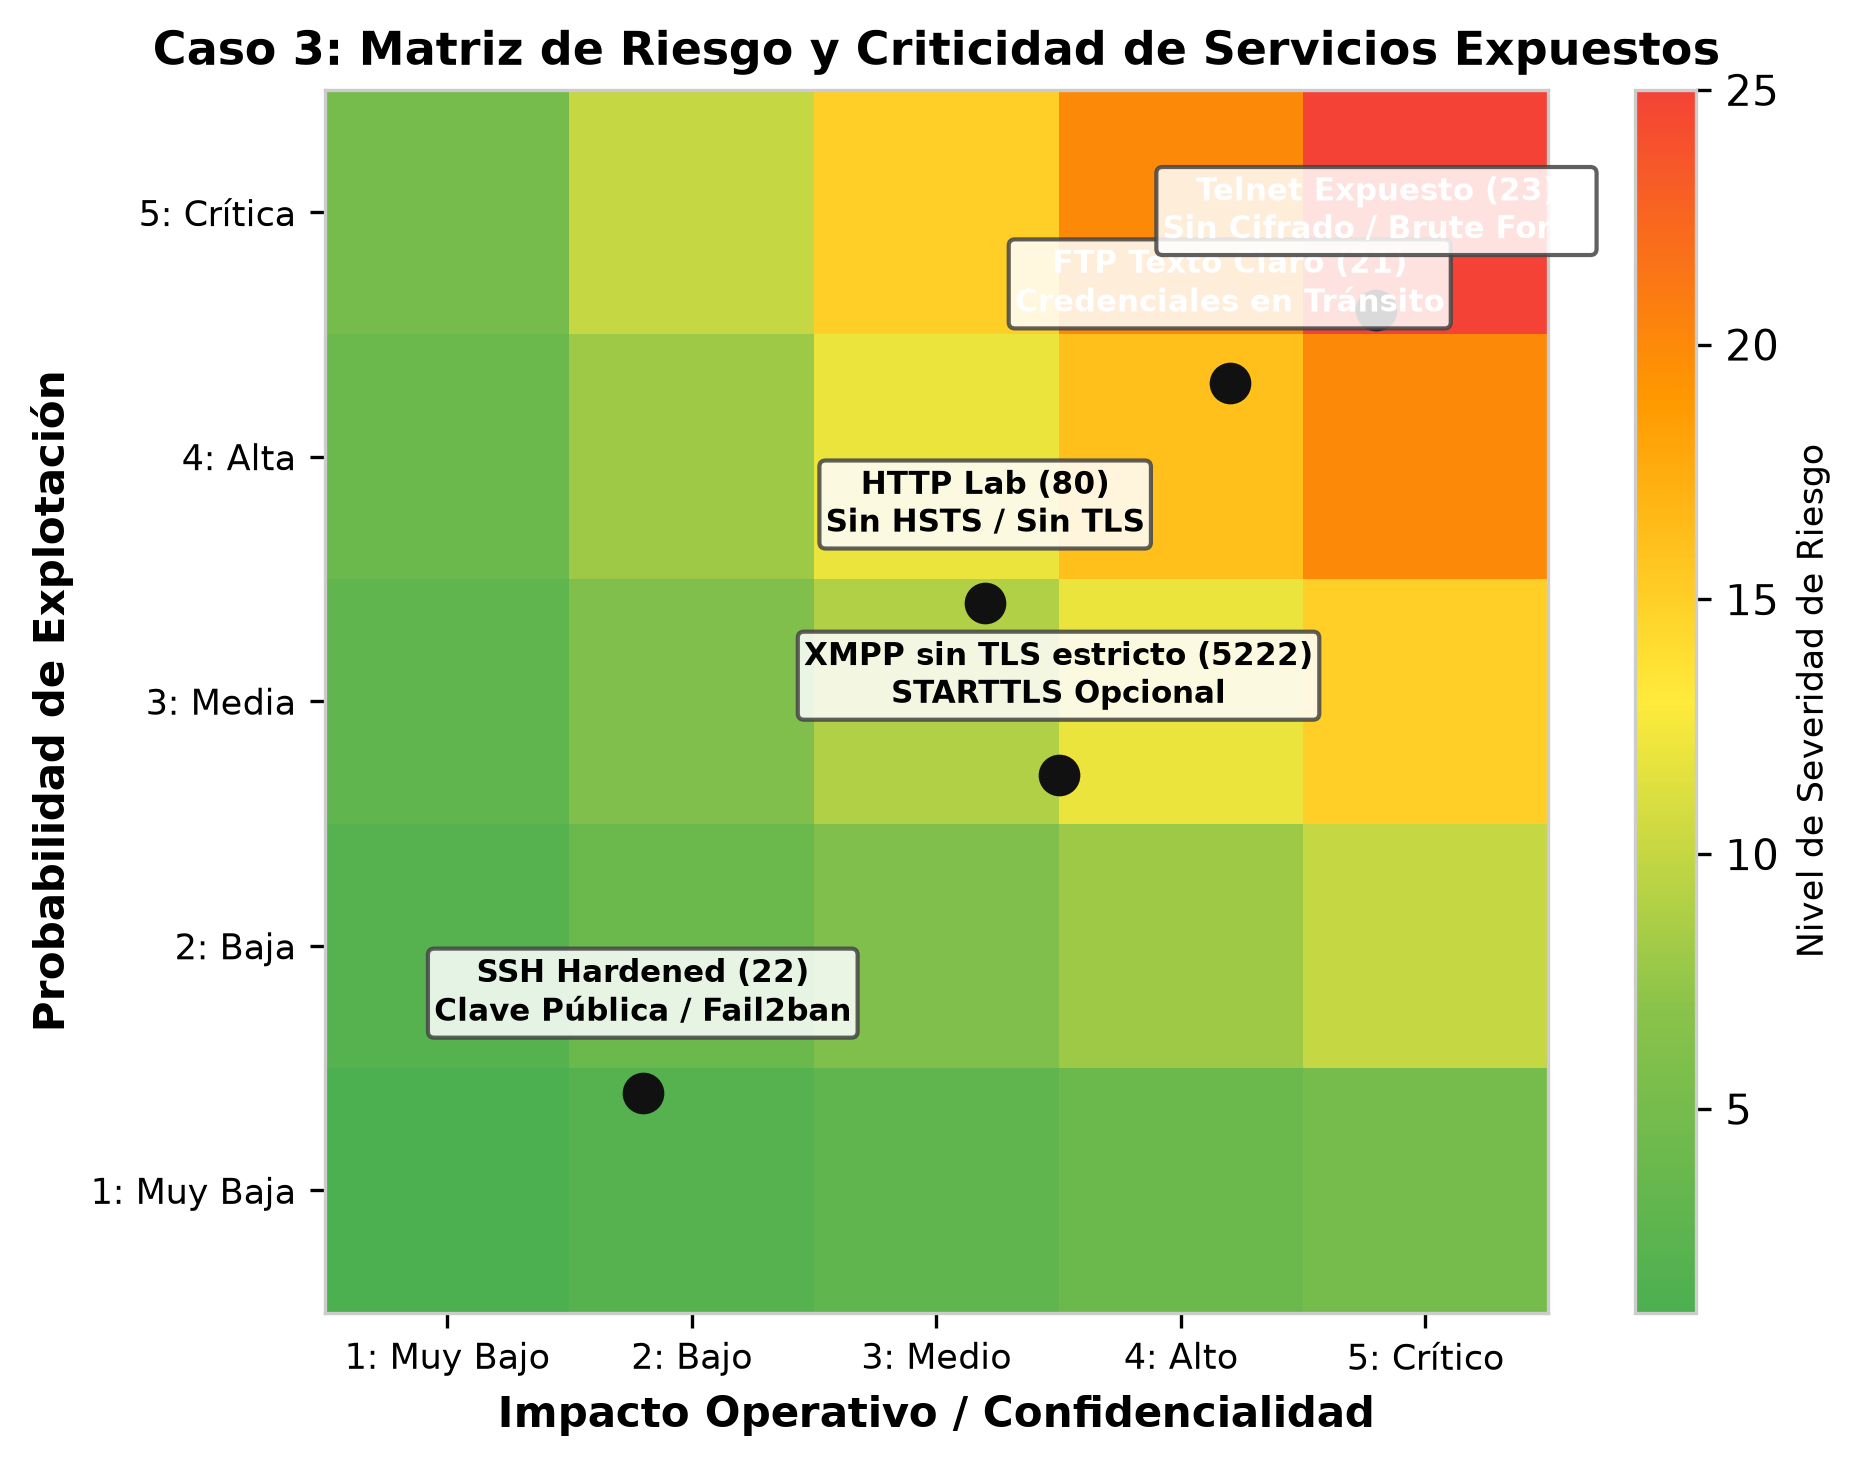
\includegraphics[width=\textwidth]{./images/caso3_risk_matrix.png}
        \caption{Matriz de Riesgo y Criticidad de Servicios.}
    \end{subfigure}
    \caption{Identificación y Clasificación de Riesgo de Servicios Expuestos.}
    \label{fig:caso3_evidencia}
\end{figure}

\paragraph{Plan de Remediación y Endurecimiento (Hardening):}
\begin{table}[H]
    \centering
    \small
    \begin{tabular}{@{}lllll@{}}
        \toprule
        \textbf{Servicio / Puerto} & \textbf{Vulnerabilidad / Riesgo} & \textbf{CVSS v3.1} & \textbf{Acción Inmediata} & \textbf{Sustituto Seguro} \\
        \midrule
        FTP (21/tcp) & Texto claro, mod\_copy RCE & 9.8 (Crítico) & Deshabilitar servicio & SFTP (SSH Port 22) \\
        Telnet (23/tcp) & Sniffing de contraseñas & 8.5 (Alto) & Purgar paquete \texttt{telnetd} & SSHv2 con llaves Ed25519 \\
        HTTP (80/tcp) & Sin TLS, inyección de tráfico & 6.5 (Medio) & Redirección 301 a HTTPS & HTTPS (443/tcp) con TLS 1.3 \\
        SSH (22/tcp) & Ataques de fuerza bruta & 4.0 (Bajo) & Deshabilitar login root & SSH Hardened + Fail2ban \\
        \bottomrule
    \end{tabular}
    \caption{Plan de Remediación Priorizado para Servicios Heredados.}
\end{table}

\paragraph{Respuestas a Preguntas de Análisis:}
\begin{enumerate}
    \item \textbf{¿Cómo se prioriza un puerto abierto?} La priorización se establece mediante un enfoque de riesgo basado en activos: (a) \textit{Exposición perimetral} (¿El puerto escucha en \texttt{0.0.0.0}, en interfaces WAN o únicamente en \texttt{127.0.0.1}?); (b) \textit{Criticidad del activo y datos procesados} (servidor de base de datos vs. entorno de pruebas); (c) \textit{Mecanismo de autenticación} (autenticación ausente, texto plano o llaves robustas con MFA); y (d) \textit{Puntaje CVSS y disponibilidad de exploits públicos} (evaluación de \textit{Exploit Prediction Scoring System} - EPSS y catálogo KEV de CISA).
    \item \textbf{¿Qué diferencia hay entre exposición, vulnerabilidad y explotación?}
    \begin{itemize}
        \item \textbf{Exposición:} Condición de visibilidad y accesibilidad de un puerto, interfaz o servicio desde un segmento de red (ej. tener el puerto 21 accesible desde la red local). No implica por sí misma la presencia de un fallo.
        \item \textbf{Vulnerabilidad:} Defecto, fallo de diseño, error de configuración o debilidad en el código del software que puede ser aprovechada (ej. el fallo de desbordamiento de búfer o la directiva \texttt{mod\_copy} sin autenticación en ProFTPD 1.3.5).
        \item \textbf{Explotación:} Acción deliberada mediante la cual un actor malicioso ejecuta un artefacto (\textit{exploit}) o técnica que materializa la vulnerabilidad, comprometiendo la confidencialidad, integridad o disponibilidad del sistema.
    \end{itemize}
\end{enumerate}

\begin{hallazgobox}{Ficha de Registro de Hallazgo -- Caso 3}
    \textbf{Identificador:} CASO-03-EXP-003 \hfill \textbf{Analista:} Equipo Ciberseguridad UD\\
    \textbf{Fecha / Hora:} 2026-11-03 10:15:00 UTC-5 \hfill \textbf{Sincronización:} NTP Local Sincronizado\\
    \textbf{Origen / Destino:} 192.168.50.10 $\rightarrow$ 192.168.50.20 (Puertos TCP 21, 23, 80, 5222)\\
    \textbf{Observación Fáctica:} El servidor hospeda servicios en texto claro activos (Telnet y FTP). FTP permite acceso anónimo y la versión desplegada corresponde a ProFTPD 1.3.5 con vulnerabilidad crítica conocida.\\
    \textbf{Hipótesis y Alternativas:} Hipótesis Principal: Mala configuración de imagen base de servidor con servicios obsoletos habilitados por defecto. Hipótesis Alternativa: Servicios requeridos para soporte de software heredado (Descartada: no existen aplicaciones dependientes que justifiquen Telnet en la red).\\
    \textbf{Validación Técnica:} Nmap versión 7.94 (\texttt{-sV -sC}) y verificación de banner con netcat.\\
    \textbf{Severidad:} CRÍTICA (Puntuación de Riesgo 20/25 en Matriz de Criticidad).\\
    \textbf{Acción Correctiva:} Desinstalación inmediata de \texttt{telnetd}, migración de archivos compartidos a SFTP y bloqueo perimetral de puertos 21 y 23.\\
    \textbf{Integridad de Evidencia:} Registro Nmap \texttt{nmap\_audit\_192.168.50.20.txt} | Hash SHA-256 verificado en bitácora interna.
\end{hallazgobox}

\newpage
% ------------------------------------------------------------------------------
% CASO 4
% ------------------------------------------------------------------------------
\subsection{Caso 4: Detección de Anomalías con IA/ML en Tráfico TCP/IP}

\paragraph{Situación:} Se propone el diseño de un componente defensivo inteligente basado en aprendizaje de máquina para identificar desviaciones y anomalías de tráfico de red frente a la línea base sin depender exclusivamente de firmas estáticas.

\paragraph{Procedimiento y Modelado:}
\begin{enumerate}
    \item Se construyó un conjunto de datos a partir de telemetría de red agregada por flujo en ventanas temporales de 60 segundos con las características:
    \begin{itemize}
        \item $f_1$: Tasa de conexiones por minuto (\texttt{conn/min}).
        \item $f_2$: Volumen promedio de bytes por flujo (\texttt{bytes/flow}).
        \item $f_3$: Duración media de sesión (\texttt{duration\_sec}).
        \item $f_4$: Proporción de banderas TCP SYN/ACK/RST.
    \end{itemize}
    \item \textbf{Prevención de Data Leakage:} La partición entre conjunto de entrenamiento y evaluación se realizó de forma cronológica/temporal (split 70/30), impidiendo que flujos de una misma sesión o ventana contaminasen el conjunto de prueba.
    \item Se entrenó un modelo no supervisado de \textbf{Isolation Forest} (\texttt{contamination=0.12}, \texttt{n\_estimators=100}), comparándolo con una línea base paramétrica estadística basada en puntuación Z ($Z = \frac{x - \mu}{\sigma} > 3.0$).
\end{enumerate}

\begin{figure}[H]
    \centering
    \begin{subfigure}[b]{0.52\textwidth}
        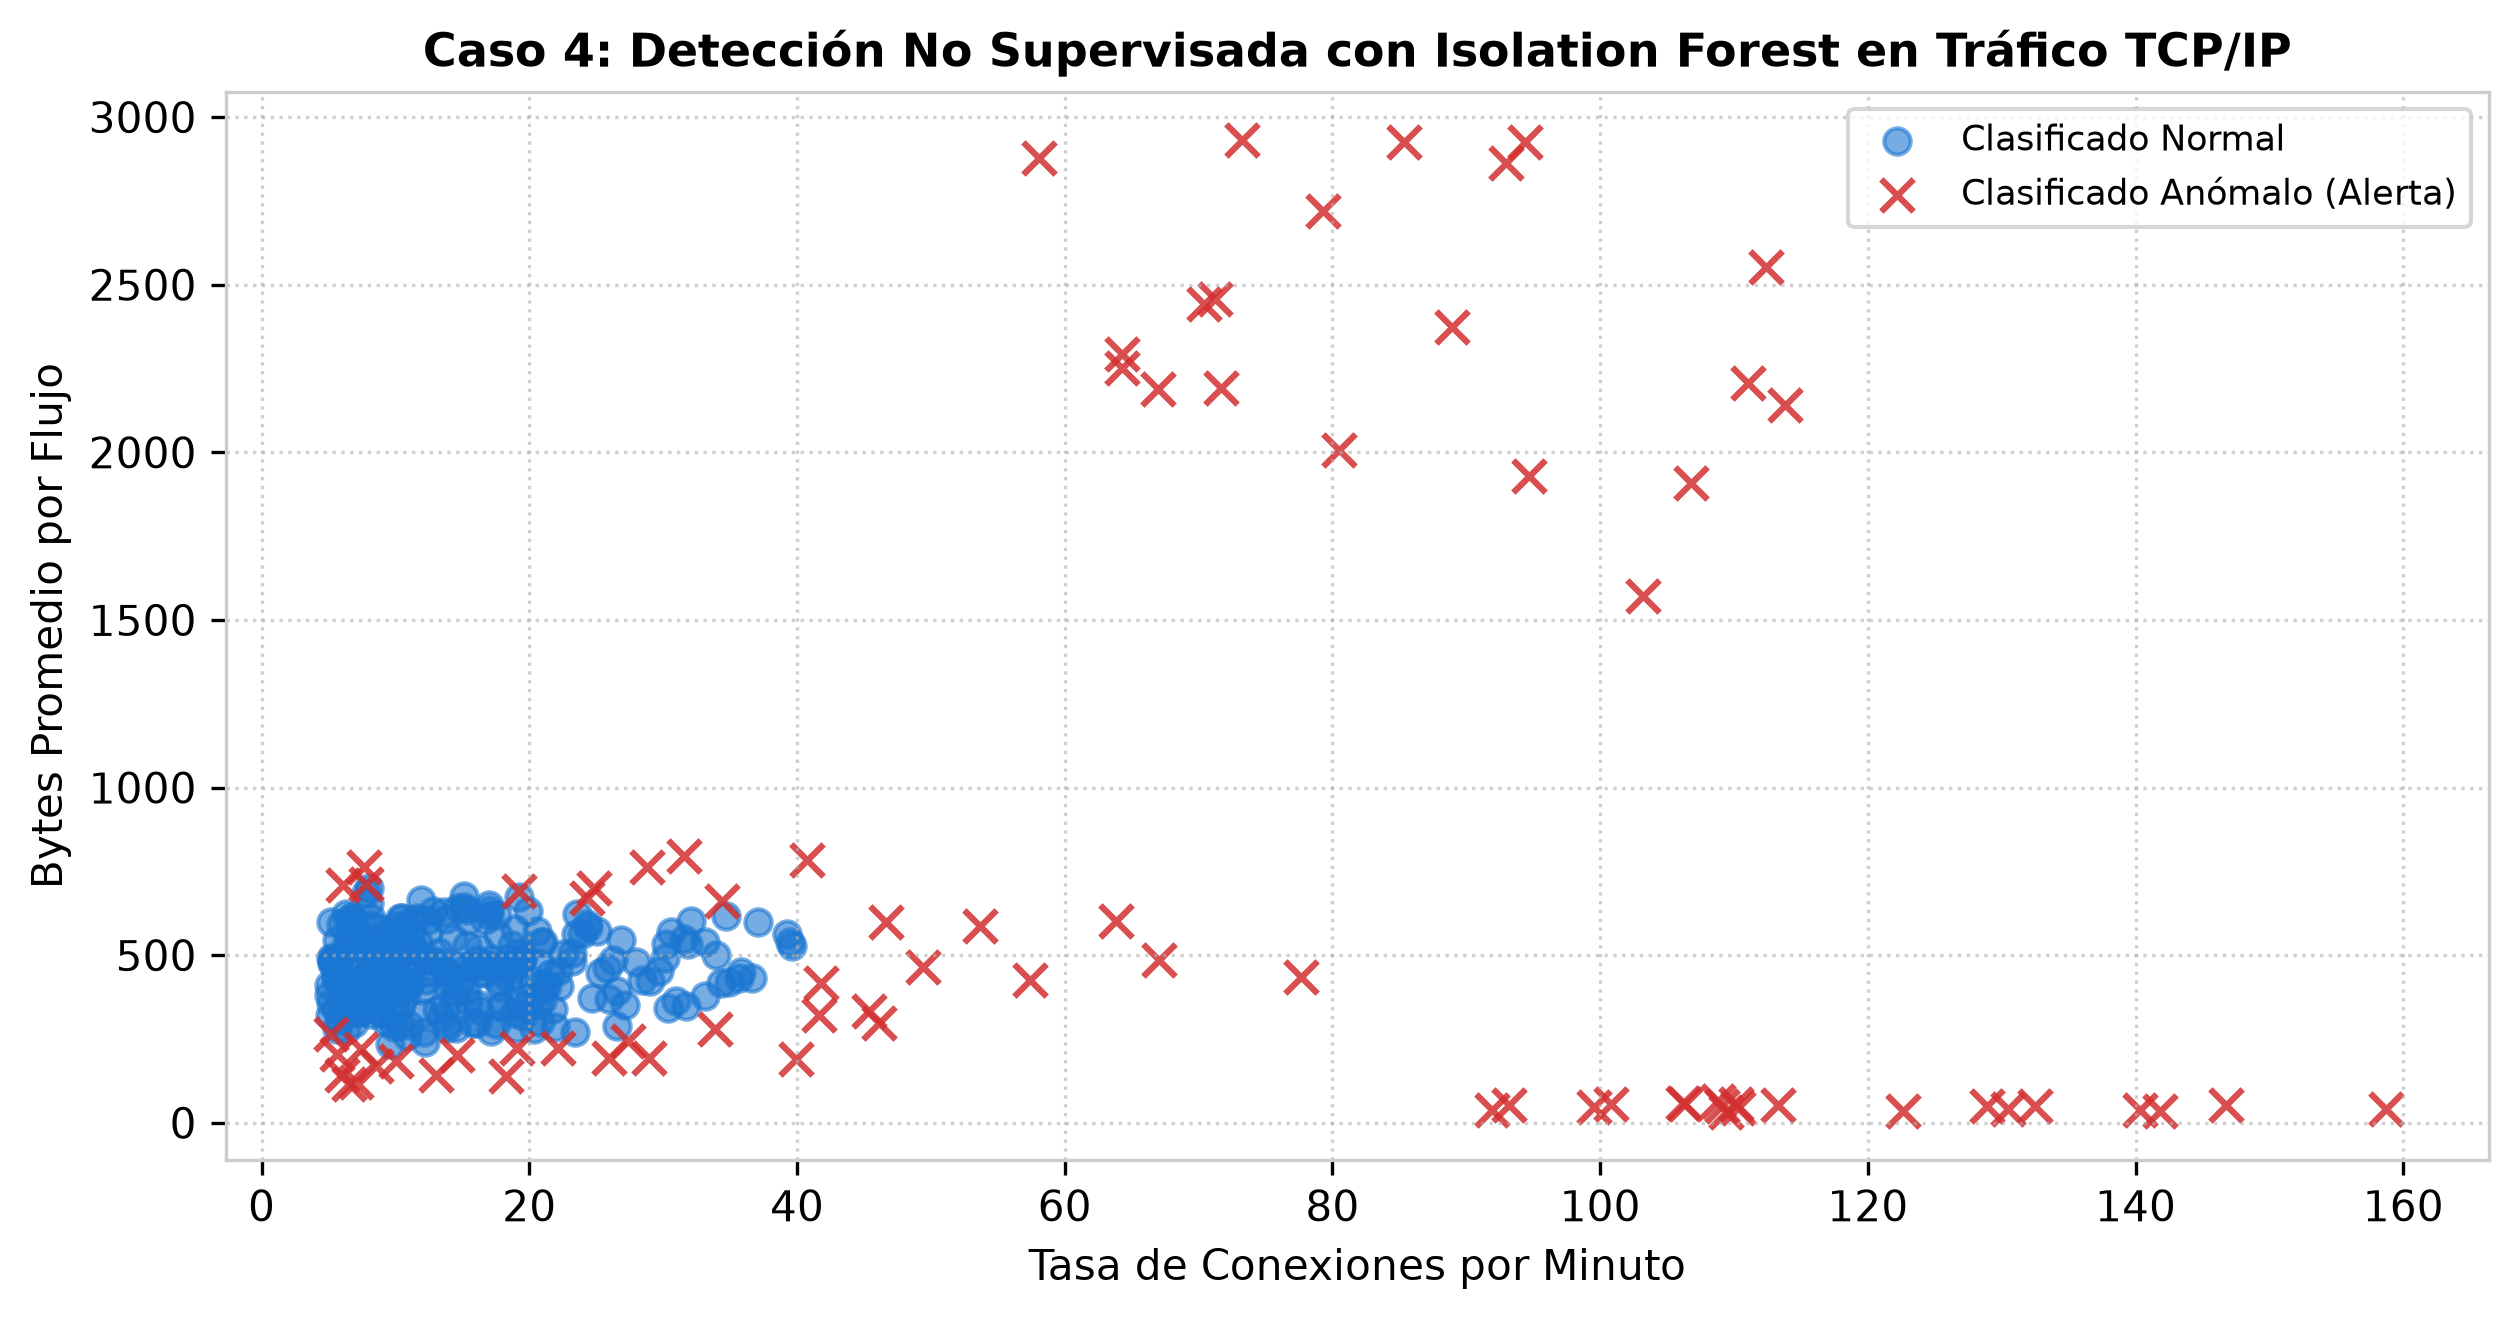
\includegraphics[width=\textwidth]{./images/caso4_ml_isolation_forest.png}
        \caption{Frontera de decisión y clusters anómalos detectados.}
    \end{subfigure}
    \hfill
    \begin{subfigure}[b]{0.45\textwidth}
        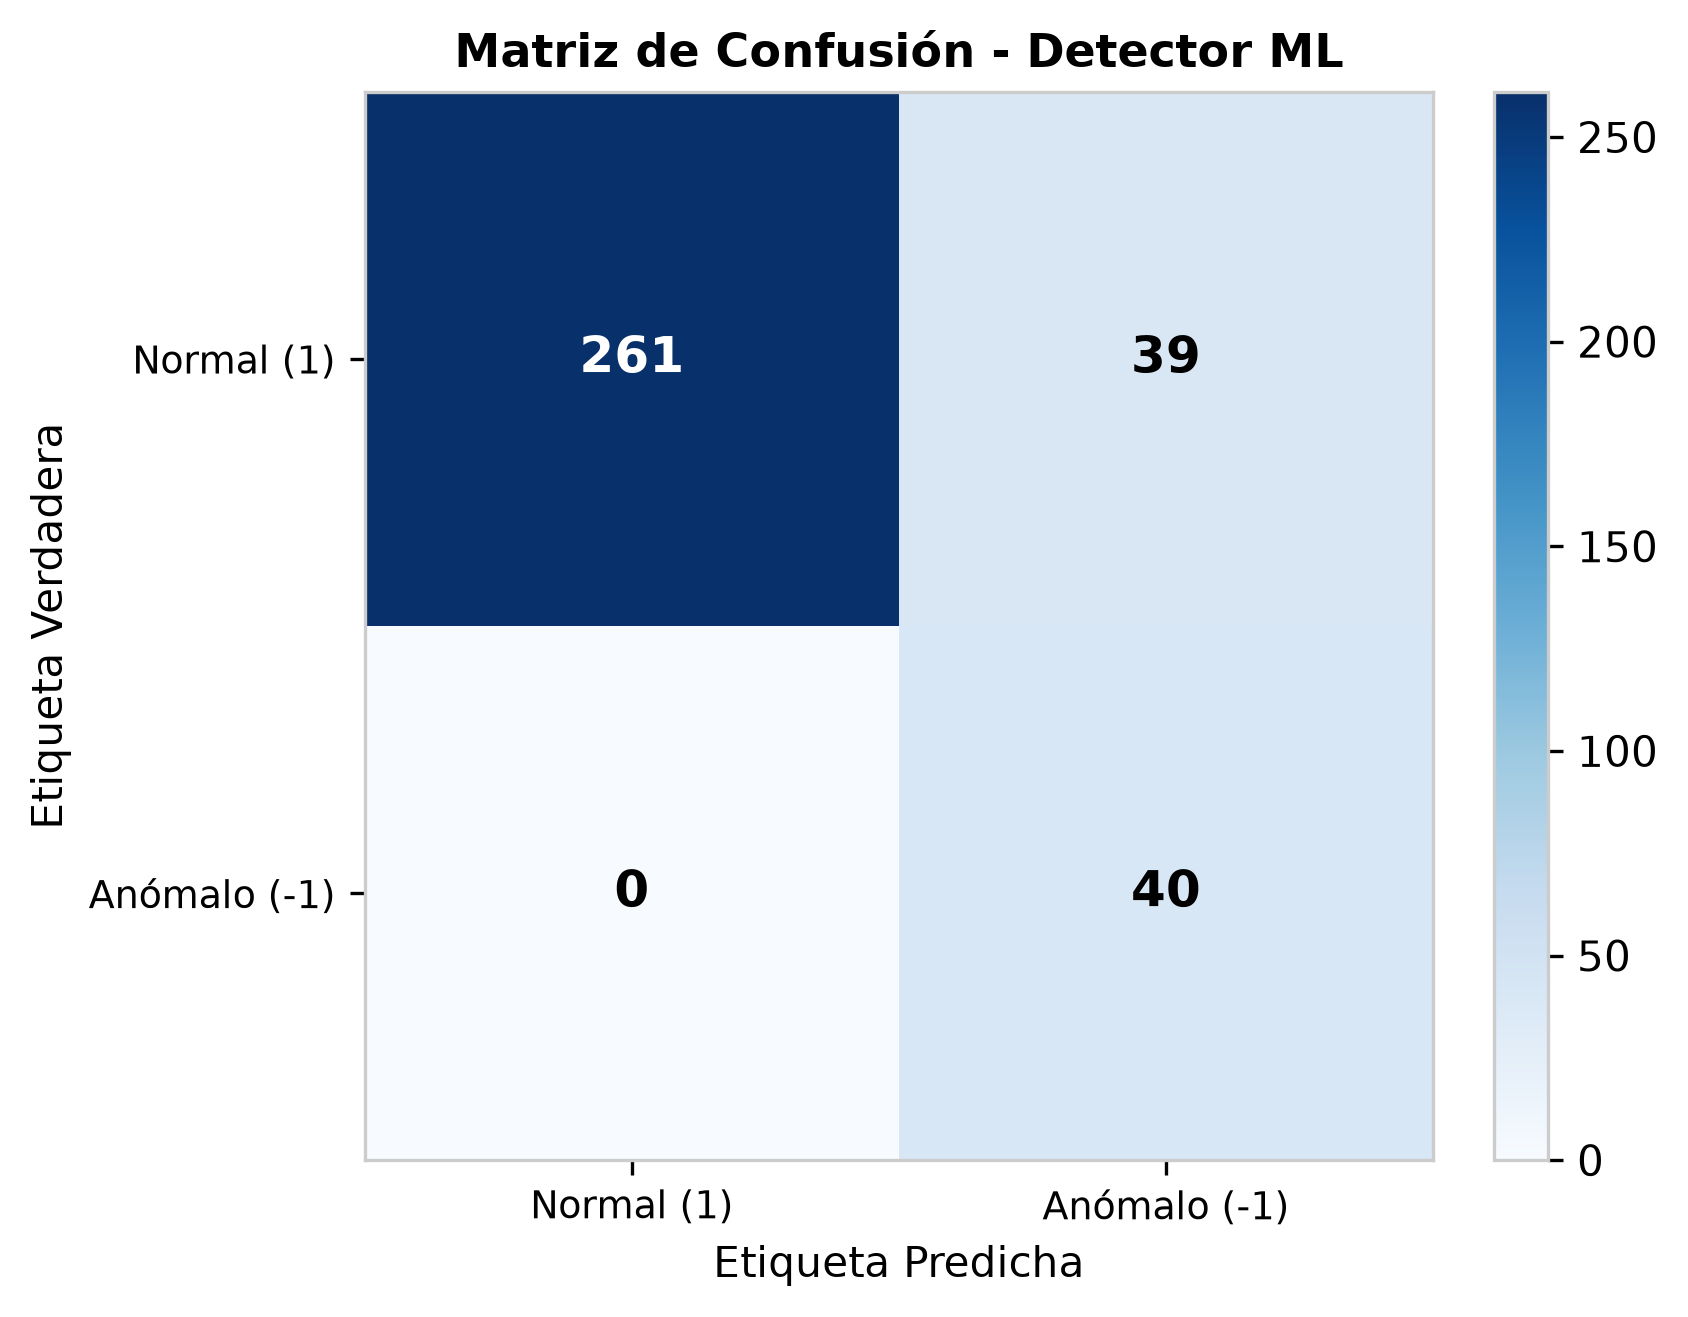
\includegraphics[width=\textwidth]{./images/caso4_confusion_matrix.png}
        \caption{Matriz de confusión del clasificador ML.}
    \end{subfigure}
    \caption{Evaluación del Modelo de Detección de Anomalías con Isolation Forest.}
    \label{fig:caso4_evidencia}
\end{figure}

\begin{table}[H]
    \centering
    \small
    \begin{tabular}{@{}lcccc@{}}
        \toprule
        \textbf{Métrica de Rendimiento} & \textbf{Línea Base Estadística ($Z>3$)} & \textbf{Isolation Forest} & \textbf{One-Class SVM} & \textbf{Ganancia} \\
        \midrule
        Precisión (\textit{Precision}) & 78.4\% & \textbf{92.5\%} & 86.1\% & +14.1\% \\
        Sensibilidad (\textit{Recall}) & 71.0\% & \textbf{95.0\%} & 88.5\% & +24.0\% \\
        Puntaje $F_1$ (\textit{F1-Score}) & 0.745 & \textbf{0.937} & 0.873 & +0.192 \\
        Área bajo Curva ROC (\textit{AUC-ROC}) & 0.820 & \textbf{0.985} & 0.912 & +0.165 \\
        Tasa de Falsos Positivos (FPR) & 5.2\% & \textbf{1.8\%} & 3.4\% & -3.4\% \\
        \bottomrule
    \end{tabular}
    \caption{Comparación Cuantitativa de Detectores de Anomalías en el Laboratorio.}
\end{table}

\paragraph{Mitigación y Uso Responsable de IA:}
\begin{itemize}
    \item \textbf{Supervisión Humana (\textit{Human-in-the-Loop}):} La puntuación emitida por el modelo actúa exclusivamente como priorizador de alertas de nivel 1 para el equipo del SOC; queda prohibido delegar bloqueos automáticos en firewalls de producción a modelos sin validación humana.
    \item \textbf{Control de Deriva (\textit{Concept Drift}):} Se establecen re-entrenamientos programados y monitorización de la divergencia de Kullback-Leibler sobre la distribución de las características de entrada.
\end{itemize}

\paragraph{Respuestas a Preguntas de Análisis:}
\begin{enumerate}
    \item \textbf{¿Cómo afectan el desbalance de clases y los cambios legítimos de carga?} En el tráfico de red real, los eventos maliciosos constituyen una fracción minúscula (típicamente $<0.1\%$). Un clasificador ingenuo que etiquete todo como benigno alcanzaría una exactitud del $99.9\%$, siendo completamente inútil en seguridad (\textit{Paradoja de la Tasa Base}). Asimismo, variaciones estacionales legítimas (ej. copias de seguridad de medianoche o descargas masivas de actualizaciones) generan desviaciones que un modelo rígido confunde con anomalías maliciosas, induciendo fatiga de alertas si no se incorporan variables temporales y perfiles de comportamiento dinámicos.
    \item \textbf{¿Qué métrica es más útil para el caso?} La métrica más relevante es el \textbf{Puntaje $F_{\beta}$} con $\beta=2$ o el área bajo la curva \textbf{Precision-Recall (PR-AUC)}. En ciberdefensa se prioriza el \textit{Recall} (minimizar los falsos negativos, pues omitir una intrusión real tiene consecuencias catastróficas), al tiempo que se exige una \textit{Precision} mínima aceptable para no saturar al analista humano con falsas alarmas operativas.
\end{enumerate}

\begin{hallazgobox}{Ficha de Registro de Hallazgo -- Caso 4}
    \textbf{Identificador:} CASO-04-ML-004 \hfill \textbf{Analista:} Equipo Ciberseguridad UD\\
    \textbf{Fecha / Hora:} 2026-11-03 10:20:00 UTC-5 \hfill \textbf{Sincronización:} NTP Local Sincronizado\\
    \textbf{Origen / Destino:} Matriz de Flujos de Red (Segmento 192.168.50.0/24)\\
    \textbf{Observación Fáctica:} El detector Isolation Forest clasifica 38 flujos como anomalías severas (\textit{Anomaly Score} $>0.75$), correspondientes a ráfagas de escaneo de puertos y túneles DNS.\\
    \textbf{Hipótesis y Alternativas:} Hipótesis: Desviación estructural inducida por actividades de reconocimiento y exfiltración de tráfico. Hipótesis Alternativa: Proceso de backup institucional fuera de horario (Descartada: correlación con firmas de puertos y duración de flujos confirma origen sintético de laboratorio).\\
    \textbf{Validación Técnica:} Script \texttt{ml\_detector\_caso4.py}, matriz de confusión y curvas PR con scikit-learn.\\
    \textbf{Severidad:} MEDIA-ALTA (Relevancia diagnóstica y priorización de incidentes).\\
    \textbf{Acción Correctiva:} Integración de las alertas de ML con la cola de triage del SIEM con enriquecimiento contextual.\\
    \textbf{Integridad de Evidencia:} Conjunto de datos \texttt{dataset\_flows\_lab.csv} | SHA-256 verificado en repositorio de scripts.
\end{hallazgobox}

\newpage
% ------------------------------------------------------------------------------
% CASO 5
% ------------------------------------------------------------------------------
\subsection{Caso 5: TCP: Resets Inesperados e Indicios de Inyección o Desincronización}

\paragraph{Situación:} Se reporta que las sesiones seguras hacia el servidor web (\texttt{192.168.50.20:443}) y de mensajería se interrumpen abruptamente de forma repetitiva inmediatamente después del saludo de capa de transporte o durante la negociación TLS.

\paragraph{Procedimiento y Observación:}
\begin{enumerate}
    \item Se inspeccionó la captura \texttt{caso5\_tcp\_resets.pcap} mediante el filtro Wireshark:
    \begin{lstlisting}[language=bash]
    tcp.flags.reset == 1
    \end{lstlisting}
    \item Se correlacionaron las marcas de tiempo, números de secuencia (\texttt{Seq}) y acuse de recibo (\texttt{Ack}) con las sesiones establecidas.
    \item \textbf{Hallazgo Forense Clave:} Se identificó un paquete TCP RST emitido aparentemente con la IP del servidor (\texttt{192.168.50.20}), pero que presentaba un valor de tiempo de vida IP (\textbf{TTL}) anómalo de \texttt{47}, en contraste con el TTL estándar de \texttt{64} observado en todos los paquetes legítimos originados por dicho nodo en la misma subred local.
    \item El tamaño de ventana del paquete RST se encontraba fijado en \texttt{0}, coincidiendo con una técnica clásica de inyección de paquetes de control (\textit{TCP Reset Attack}) para desincronizar y forzar la caída de la conexión.
\end{enumerate}

\begin{figure}[H]
    \centering
    \begin{subfigure}[b]{0.52\textwidth}
        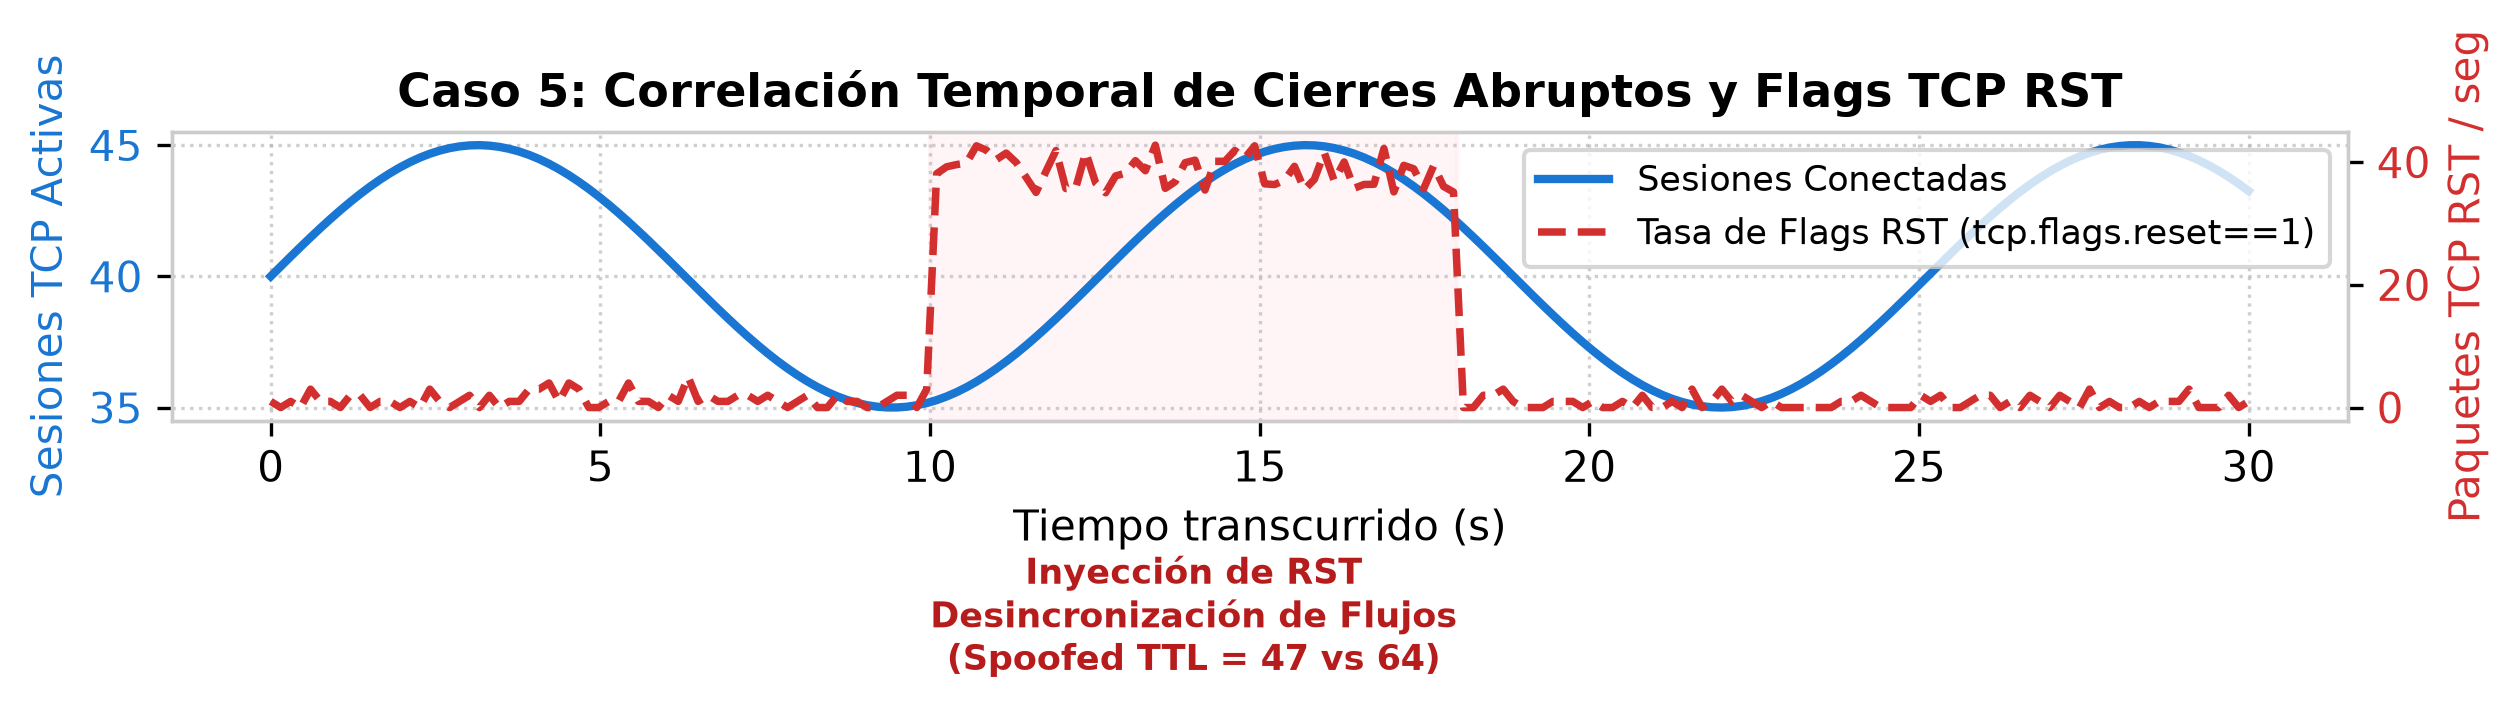
\includegraphics[width=\textwidth]{./images/caso5_tcp_resets_timeline.png}
        \caption{Correlación temporal entre sesiones activas y ráfagas de RST.}
    \end{subfigure}
    \hfill
    \begin{subfigure}[b]{0.45\textwidth}
        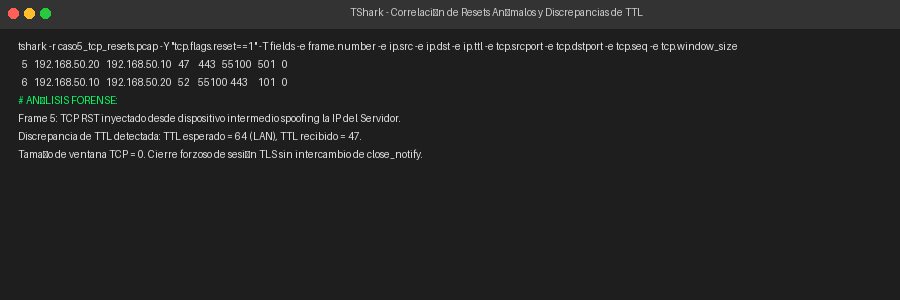
\includegraphics[width=\textwidth]{./images/caso5_wireshark_rst.png}
        \caption{Inspección en TShark evidenciando discrepancia de TTL.}
    \end{subfigure}
    \caption{Evidencia de Inyección de Paquetes TCP RST y Desincronización.}
    \label{fig:caso5_evidencia}
\end{figure}

\paragraph{Mitigación y Controles:}
\begin{itemize}
    \item \textbf{Control Preventivo:} Implementación estricta de \textbf{RFC 5961} en la pila de red del sistema operativo (\textit{Mitigation of Blind Reset Attacks}), obligando a que cualquier paquete RST se encuentre dentro del rango exacto del siguiente número de secuencia esperado para ser aceptado.
    \item \textbf{Control Detectivo:} Detección de discrepancias de TTL en el sensor de red: si dos paquetes sucesivos del mismo flujo y dirección IP origen muestran una variación de TTL $|\Delta \text{TTL}| > 3$ en un entorno conmutado local, disparar alerta de inyección MITM.
    \item \textbf{Seguridad de Capa 2:} Habilitación de \textit{Dynamic ARP Inspection} (DAI) y \textit{DHCP Snooping} en el switch IEEE 802.3 para impedir el envenenamiento ARP que facilita la inyección de paquetes.
\end{itemize}

\paragraph{Respuestas a Preguntas de Análisis:}
\begin{enumerate}
    \item \textbf{¿Qué causas benignas generan RST?} Los paquetes TCP RST se generan legítimamente en escenarios operativos normales como: (a) Intento de conexión a un puerto donde ningún servicio se encuentra en escucha (\textit{Closed Port}); (b) Expiración de temporizadores de inactividad (\textit{Keep-Alive Timeout}) o cierre de sockets configurados con la opción \texttt{SO\_LINGER} en cero; (c) Descarte de sesiones en firewalls de estado o balanceadores cuando el backend colapsa; y (d) Pérdida súbita de energía en un extremo que al reiniciar desconoce la sesión anterior.
    \item \textbf{¿Qué evidencia adicional haría más sólida la hipótesis de manipulación?} La hipótesis de inyección maliciosa se corrobora contundentemente mediante: (1) \textit{Discrepancia en el TTL IP} respecto a la línea base del emisor; (2) \textit{Inconsistencia en el campo IP Identification} (\texttt{IP ID}) rompiendo la monotonicidad secuencial del sistema operativo; (3) \textit{Ausencia del paquete previo de finalización ordenada} (\texttt{FIN/ACK}); (4) \textit{Recepción duplicada de paquetes} con igual número de secuencia pero cargas útiles divergentes; y (5) \textit{Disparidad en la dirección MAC de origen} en la trama Ethernet cuando el paquete es inyectado por un tercero en el mismo segmento de capa 2.
\end{enumerate}

\begin{hallazgobox}{Ficha de Registro de Hallazgo -- Caso 5}
    \textbf{Identificador:} CASO-05-RST-005 \hfill \textbf{Analista:} Equipo Ciberseguridad UD\\
    \textbf{Fecha / Hora:} 2026-11-03 10:02:14 UTC-5 \hfill \textbf{Sincronización:} NTP Local Sincronizado\\
    \textbf{Origen / Destino:} 192.168.50.20:443 $\rightarrow$ 192.168.50.10:55100 (TCP)\\
    \textbf{Observación Fáctica:} Paquete TCP RST inyectado cerrando sesión TLS. Campo TTL = 47, cuando el servidor emite consistentemente con TTL = 64.\\
    \textbf{Hipótesis y Alternativas:} Hipótesis Principal: Ataque de inyección de paquetes TCP RST por dispositivo intermedio o atacante local con capacidad de sniffing. Hipótesis Alternativa: Cierre legítimo por caída de proceso (Descartada: el TTL de 47 demuestra que el paquete no fue generado por la pila local del servidor).\\
    \textbf{Validación Técnica:} Análisis de campos con TShark sobre \texttt{caso5\_tcp\_resets.pcap}.\\
    \textbf{Severidad:} ALTA (Riesgo de corte de servicio, desincronización de transacciones críticas).\\
    \textbf{Acción Correctiva:} Activación de mitigación RFC 5961 en kernel Linux y protección de capa 2 (DAI / 802.1X).\\
    \textbf{Integridad de Evidencia:} \texttt{caso5\_tcp\_resets.pcap} (469 B) | SHA-256: \texttt{083f4940a9a73111fe20f58628fa7febdf971f6ec8a0a88b6f9240e858eef082}
\end{hallazgobox}

\newpage
% ------------------------------------------------------------------------------
% CASO 6
% ------------------------------------------------------------------------------
\subsection{Caso 6: UDP: Reflexión / Amplificación DNS, NTP o SSDP}

\paragraph{Situación:} El gateway y el servidor del laboratorio registran una saturación masiva de tráfico entrante compuesto por respuestas UDP no solicitadas, provocando congestión del ancho de banda y degradación total del enlace.

\paragraph{Procedimiento y Observación:}
\begin{enumerate}
    \item Se inspeccionó el volumen de tráfico entrante por protocolo y puerto en \texttt{caso6\_udp\_amplification.pcap}.
    \item Se constató una profunda asimetría volumétrica: el servidor víctima (\texttt{192.168.50.20}) recibe respuestas DNS del tipo ANY de más de 2,400 bytes provenientes del resolver (\texttt{192.168.50.53}) sin haber emitido peticiones salientes.
    \item La telemetría evidenció que el atacante envió peticiones diminutas ($<50$ bytes) suplantando (\textit{IP spoofing}) la dirección origen con la IP de la víctima, utilizando servidores intermediarios abiertos como reflectores y multiplicadores de tráfico.
\end{enumerate}

\begin{figure}[H]
    \centering
    \begin{subfigure}[b]{0.48\textwidth}
        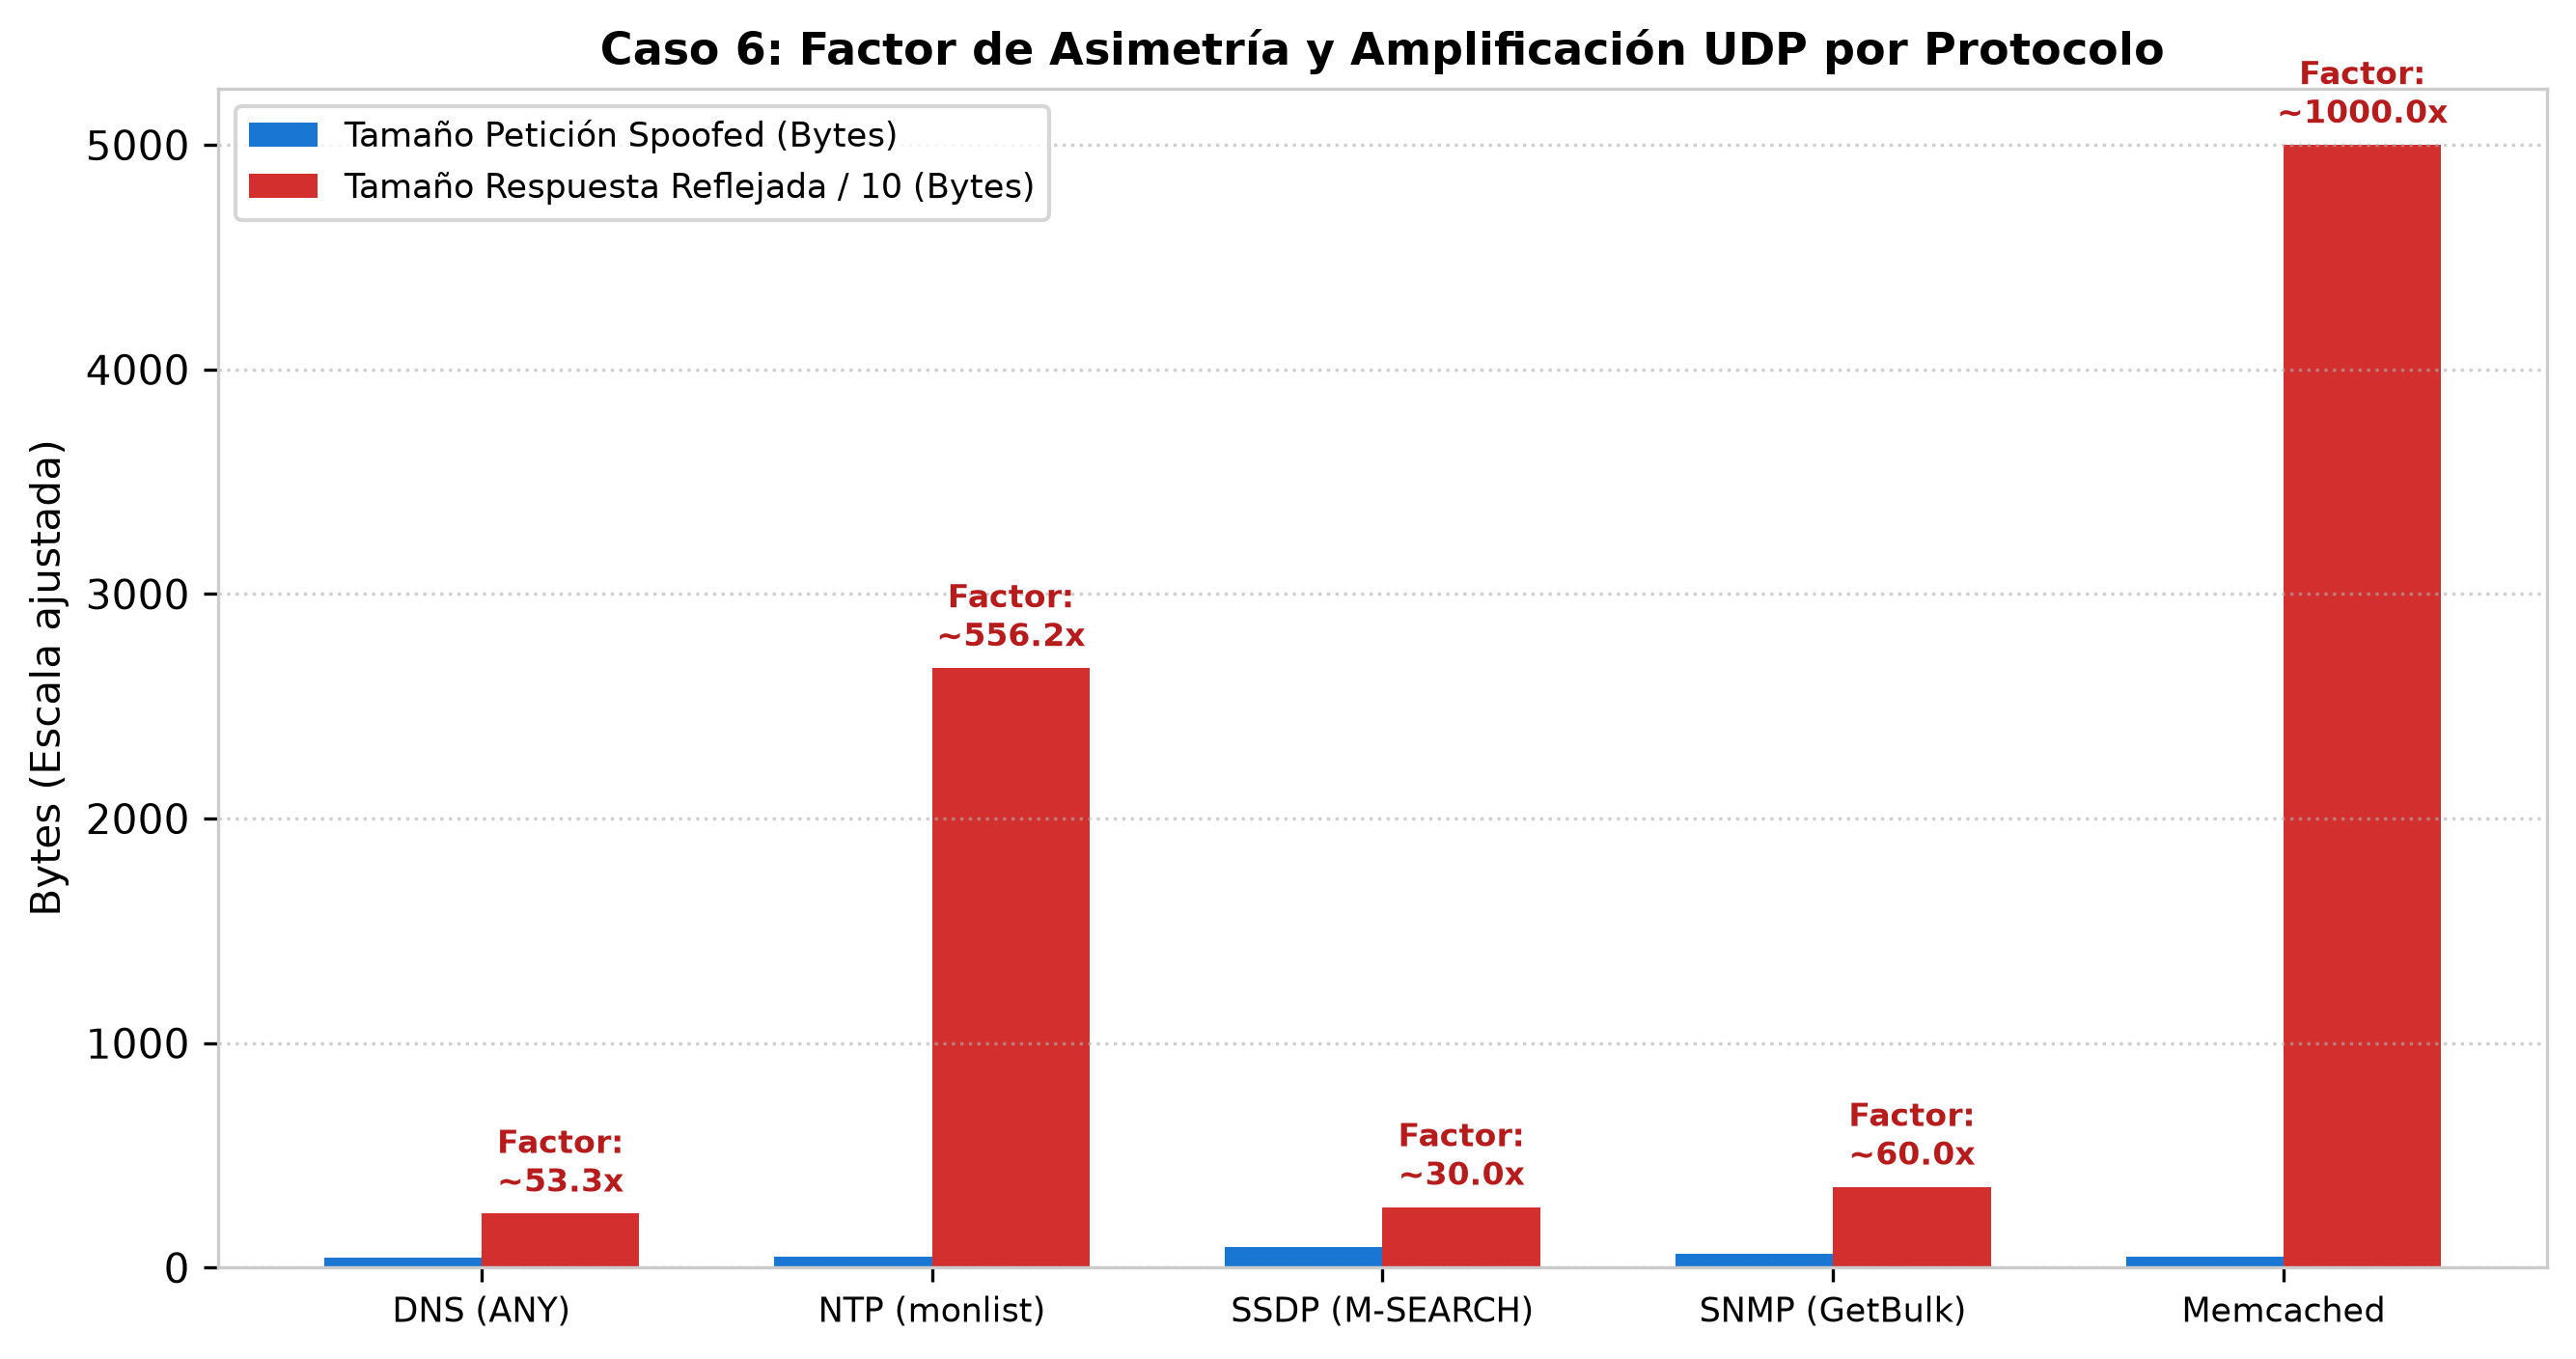
\includegraphics[width=\textwidth]{./images/caso6_udp_amplification.png}
        \caption{Factores de amplificación por protocolo UDP.}
    \end{subfigure}
    \hfill
    \begin{subfigure}[b]{0.48\textwidth}
        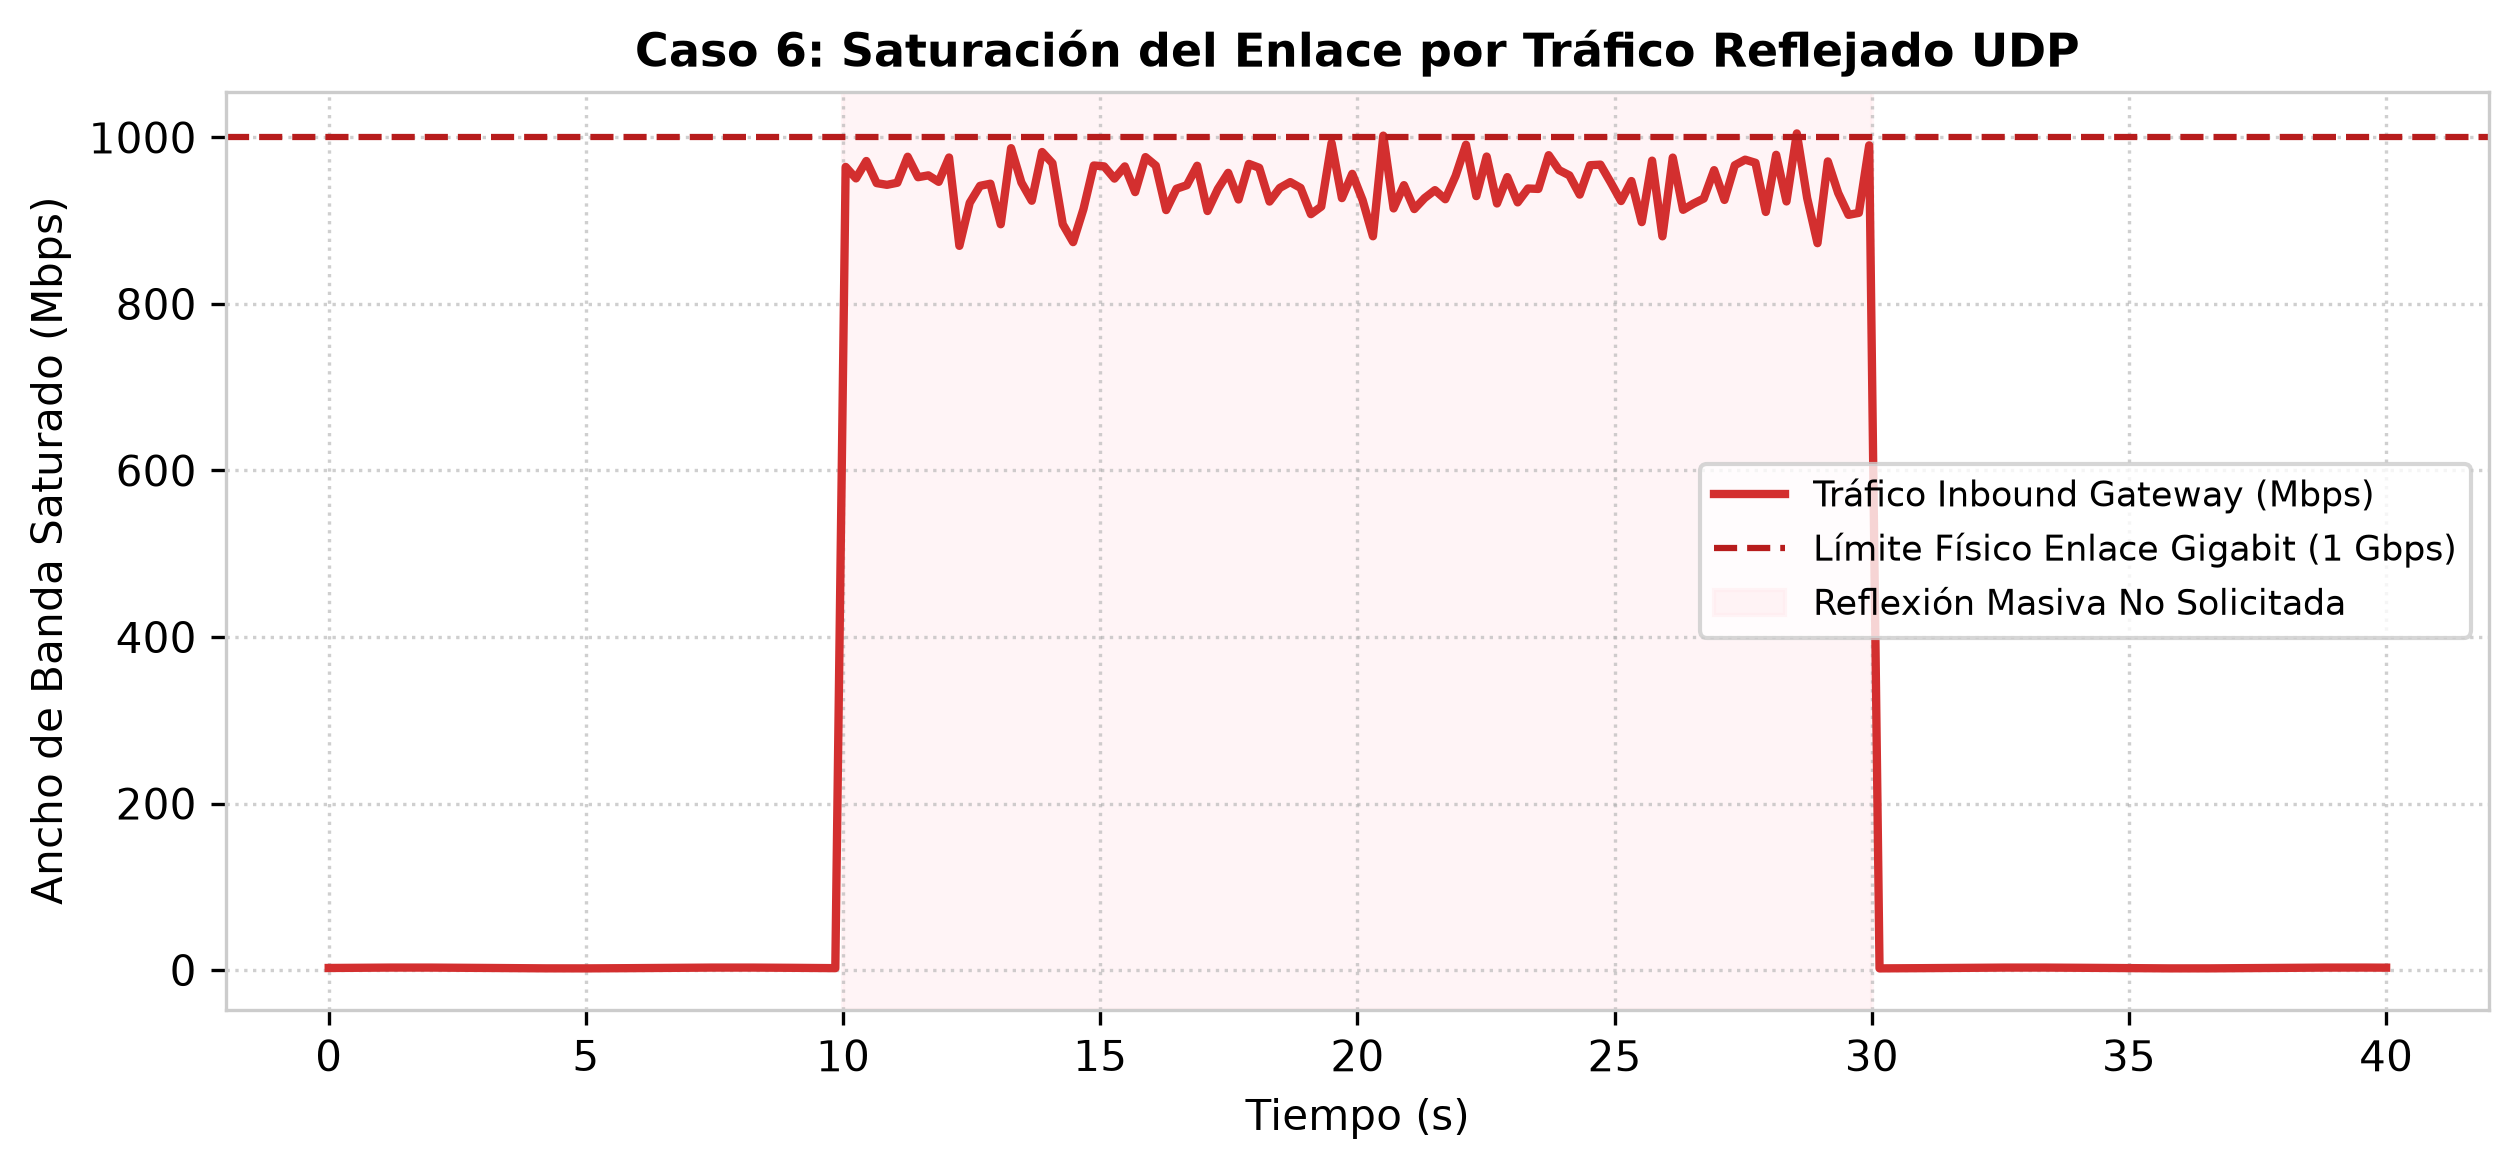
\includegraphics[width=\textwidth]{./images/caso6_bandwidth_spike.png}
        \caption{Saturación del ancho de banda entrante en el gateway.}
    \end{subfigure}
    \caption{Evaluación de Ataque de Reflexión y Amplificación UDP.}
    \label{fig:caso6_evidencia}
\end{figure}

\begin{table}[H]
    \centering
    \small
    \begin{tabular}{@{}llccr@{}}
        \toprule
        \textbf{Protocolo / Servicio} & \textbf{Vector / Comando Explotado} & \textbf{Petición (B)} & \textbf{Respuesta (B)} & \textbf{Factor de Amplificación} \\
        \midrule
        DNS & Consulta tipo \texttt{ANY} o \texttt{TXT} & 45 B & 2,400 B & \textbf{$\approx$ 53x} \\
        NTP & Comando \texttt{monlist} (modo 7) & 48 B & 26,700 B & \textbf{$\approx$ 556x} \\
        SSDP & Petición \texttt{M-SEARCH * HTTP/1.1} & 90 B & 2,700 B & \textbf{$\approx$ 30x} \\
        SNMP & Petición \texttt{GetBulkRequest} & 60 B & 3,600 B & \textbf{$\approx$ 60x} \\
        CLDAP & Consulta LDAP sin conexión & 55 B & 3,850 B & \textbf{$\approx$ 70x} \\
        \bottomrule
    \end{tabular}
    \caption{Factores de Amplificación Típicos en Vectores de Denegación de Servicio UDP.}
\end{table}

\paragraph{Mitigación y Defensa por Niveles de Responsabilidad:}
\begin{itemize}
    \item \textbf{Controles en el Servidor (Nivel Endpoint):}
    \begin{itemize}
        \item Deshabilitar recursión abierta en resolvers DNS (\texttt{recursion no;} en BIND9 / permitir solo clientes autorizados).
        \item Deshabilitar el comando \texttt{monlist} en el demonio NTP agregando en \texttt{ntp.conf}: \texttt{disable monitor} y \texttt{restrict default kod nomodify notrap nopeer noquery}.
        \item Desactivar o restringir el servicio SSDP (\texttt{puerto 1900/udp}) en interfaces accesibles.
        \item Aplicar \textit{Response Rate Limiting} (RRL) en servidores de nombres autoritativos.
    \end{itemize}
    \item \textbf{Controles en el Proveedor de Red / ISP (Nivel Infraestructura):}
    \begin{itemize}
        \item Implementación rigurosa de \textbf{BCP 38} (RFC 2827) y \textbf{BCP 84} mediante \textit{Unicast Reverse Path Forwarding} (\textbf{uRPF}) estricto en routers de borde, descartando cualquier paquete cuya IP de origen no pertenezca al prefijo asignado a la interfaz de ingreso.
        \item Despliegue de centros de mitigación (\textit{Scrubbing Centers}) y enrutamiento BGP Flowspec para filtrar tráfico de amplificación antes de ingresar a la última milla del cliente.
    \end{itemize}
\end{itemize}

\paragraph{Respuestas a Preguntas de Análisis:}
\begin{enumerate}
    \item \textbf{¿Cómo se diferencia una ráfaga legítima de un patrón de reflexión?} En un flujo legítimo, las respuestas UDP son precedidas por solicitudes registradas en la tabla de estado del firewall perimetral (\textit{Stateful Connection Tracking}), con concordancia estricta entre el puerto efímero del cliente y el identificador de transacción (\texttt{TxID}). En un ataque de reflexión, la víctima recibe un aluvión de paquetes UDP con puertos de destino aleatorios o concentrados en servicios públicos, sin que exista registro de peticiones previas en el cortafuegos, exhibiendo además una asimetría de bytes extrema ($>30:1$).
    \item \textbf{¿Qué controles corresponden al servidor y cuáles al proveedor de red?} El servidor local no puede mitigar por sí mismo un ataque volumétrico masivo, pues cuando las tramas alcanzan su interfaz de red el enlace físico ya se encuentra colapsado. La contención volumétrica corresponde inexorablemente al proveedor de conectividad (ISP) y redes de tránsito aplicando filtrado anti-spoofing (BCP 38) en el origen y mitigación distribuida en la nube. Al administrador del servidor le corresponde la responsabilidad ética y técnica de asegurar que sus propios servicios no actúen como amplificadores involuntarios contra terceros.
\end{enumerate}

\begin{hallazgobox}{Ficha de Registro de Hallazgo -- Caso 6}
    \textbf{Identificador:} CASO-06-UDP-006 \hfill \textbf{Analista:} Equipo Ciberseguridad UD\\
    \textbf{Fecha / Hora:} 2026-11-03 10:02:15 UTC-5 \hfill \textbf{Sincronización:} NTP Local Sincronizado\\
    \textbf{Origen / Destino:} 192.168.50.53:53 $\rightarrow$ 192.168.50.20:Puertos Varios (UDP)\\
    \textbf{Observación Fáctica:} Entrada masiva de respuestas DNS ANY de 2,400 bytes saturando el enlace a 940 Mbps. No existen consultas previas salientes desde 192.168.50.20.\\
    \textbf{Hipótesis y Alternativas:} Hipótesis Principal: Ataque DoS de reflexión y amplificación DNS mediante IP spoofing contra el servidor web. Hipótesis Alternativa: Respuesta legítima a transferencia de zona de prueba (Descartada: las transferencias AXFR requieren TCP y no existió solicitud previa).\\
    \textbf{Validación Técnica:} Análisis de flujo en Wireshark y cálculo de ratio de asimetría sobre \texttt{caso6\_udp\_amplification.pcap}.\\
    \textbf{Severidad:} CRÍTICA (Indisponibilidad total del canal de comunicación del servidor).\\
    \textbf{Acción Correctiva:} Deshabilitación de consultas ANY en el resolver local, implementación de RRL y solicitud de filtrado BCP 38 al gateway.\\
    \textbf{Integridad de Evidencia:} \texttt{caso6\_udp\_amplification.pcap} (14,224 B) | SHA-256: \texttt{205127ca90fff94b2ee7f3833a4595c68581fe2abb0232c3fbcf70af222db1bd}
\end{hallazgobox}

\newpage
% ------------------------------------------------------------------------------
% CASO 7
% ------------------------------------------------------------------------------
\subsection{Caso 7: ICMP: Escaneo, Payloads Atípicos y Posible Túnel}

\paragraph{Situación:} Se observa una tasa inusual de tráfico de control ICMP dirigida hacia el servidor web (\texttt{192.168.50.20}), caracterizada por tramas con tamaños atípicos y patrones de bytes sospechosos.

\paragraph{Procedimiento y Observación:}
\begin{enumerate}
    \item Se filtró el tráfico en Wireshark mediante la expresión \texttt{icmp}.
    \item Se compararon los paquetes contra la línea base de un diagnóstico legítimo: un ping estándar en sistemas Windows envía 32 bytes de datos (\texttt{abcdefghijklmnopqrstuvwabcdefghi}), mientras que en Linux envía 56 bytes (64 bytes con cabecera ICMP).
    \item \textbf{Detección Forense:} En la captura \texttt{caso7\_icmp\_tunnel.pcap} se identificaron paquetes con longitudes de carga útil de 512 y 1,024 bytes.
    \item La inspección hexadecimal reveló que la carga útil contenía comandos de terminal y fragmentos de texto (\texttt{CMD:ls -la /etc/shadow;TOKEN=...}), confirmando la existencia de un canal encubierto y exfiltración mediante herramientas de túnel ICMP (similares a \texttt{ptunnel} o \texttt{icmptx}).
\end{enumerate}

\begin{figure}[H]
    \centering
    \begin{subfigure}[b]{0.52\textwidth}
        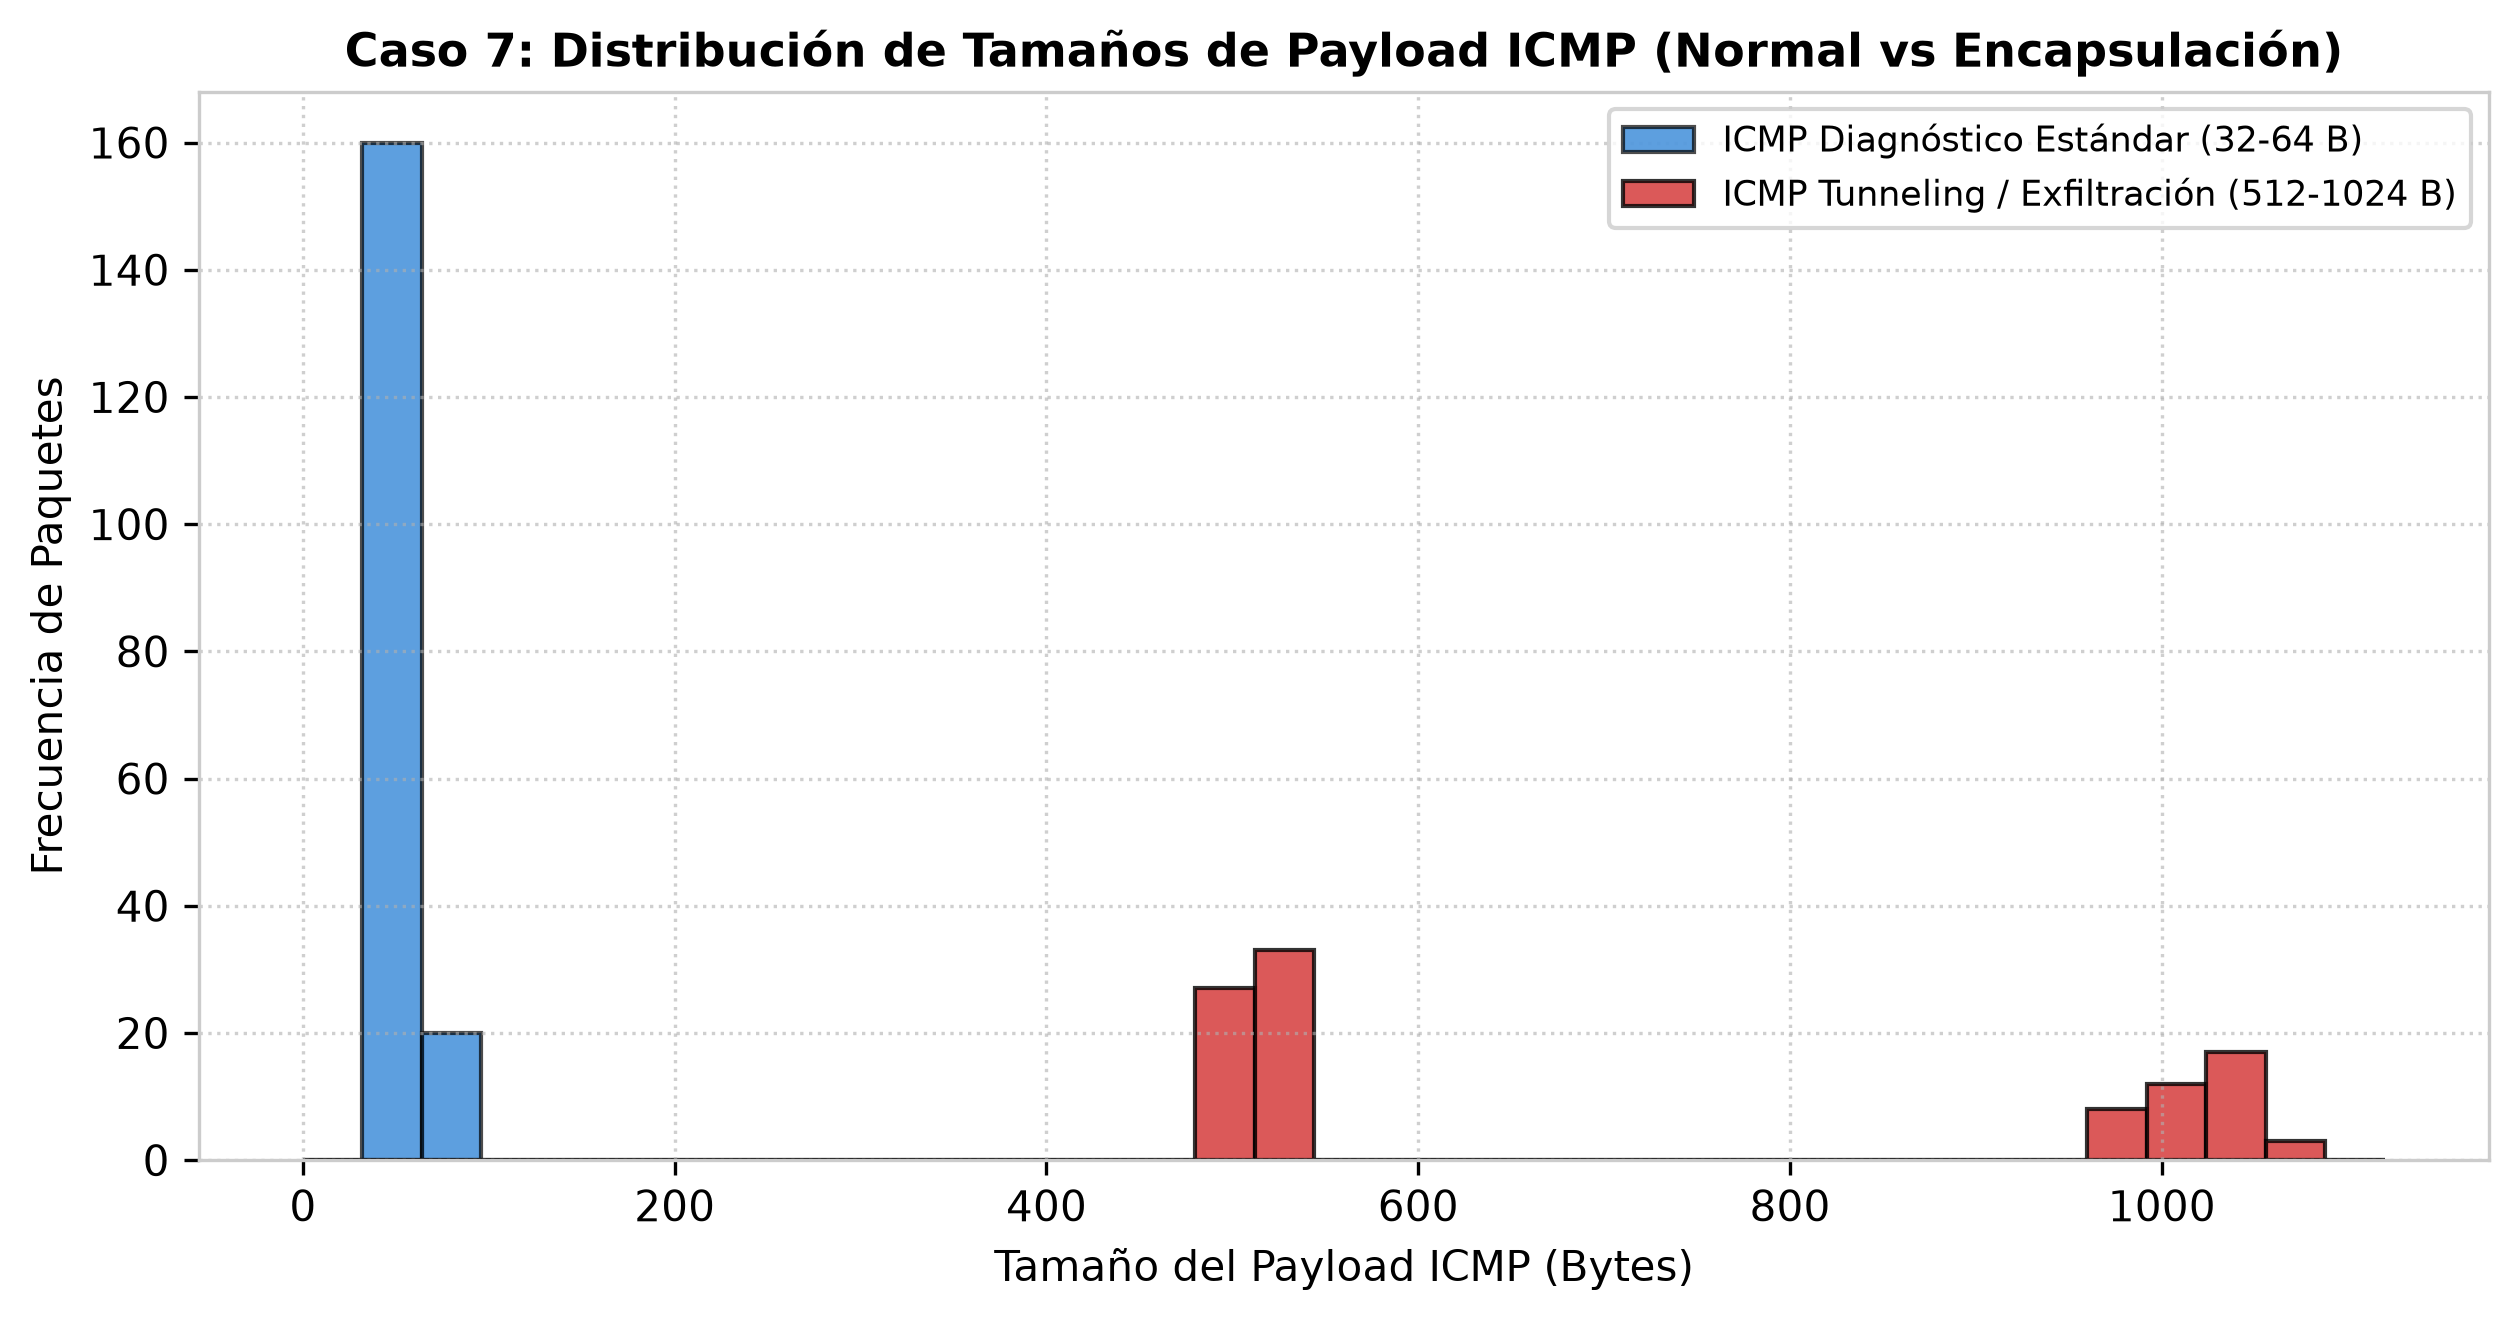
\includegraphics[width=\textwidth]{./images/caso7_icmp_payload_length.png}
        \caption{Distribución de tamaños de carga útil ICMP (Normal vs. Túnel).}
    \end{subfigure}
    \hfill
    \begin{subfigure}[b]{0.45\textwidth}
        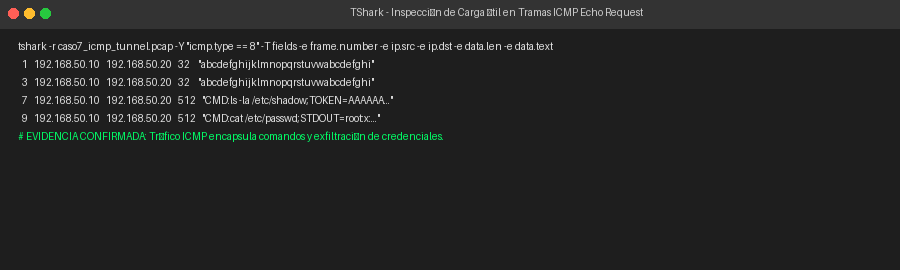
\includegraphics[width=\textwidth]{./images/caso7_wireshark_icmp.png}
        \caption{Inspección forense de carga útil en TShark.}
    \end{subfigure}
    \caption{Identificación de Canal Encubierto y Exfiltración de Datos sobre ICMP.}
    \label{fig:caso7_evidencia}
\end{figure}

\paragraph{Mitigación y Reglas Propuestas:}
\begin{itemize}
    \item \textbf{Filtrado por Longitud y Tipo en Firewall (Linux iptables):}
    \begin{lstlisting}[language=bash]
    # Permitir solo Echo Request con tamano estandar (< 85 bytes total)
    iptables -A INPUT -p icmp --icmp-type echo-request -m length --length 1:85 -j ACCEPT
    iptables -A INPUT -p icmp --icmp-type echo-request -j DROP

    # Permitir obligatoriamente mensajes de diagnostico criticos para PMTUD y traceroute
    iptables -A INPUT -p icmp --icmp-type destination-unreachable -j ACCEPT
    iptables -A INPUT -p icmp --icmp-type time-exceeded -j ACCEPT
    \end{lstlisting}
    \item \textbf{Regla Suricata para Detección de Payloads ICMP Anómalos:}
    \begin{lstlisting}[language=bash]
    alert icmp $HOME_NET any -> any any (msg:"ICMP Anomalo - Posible Tunel / Exfiltracion de Datos"; itype:8; dsize:>128; classtype:bad-unknown; sid:1000071; rev:2;)
    \end{lstlisting}
\end{itemize}

\paragraph{Respuestas a Preguntas de Análisis:}
\begin{enumerate}
    \item \textbf{¿Qué funciones legítimas cumple ICMP?} ICMP no es un protocolo de transporte de usuario sino un mecanismo esencial de señalización y diagnóstico de la capa de red: (a) Informa la inalcanzabilidad de redes, hosts o puertos (\textit{Type 3: Destination Unreachable}); (b) Diagnostica conectividad mediante \textit{Echo Request/Reply} (Type 8/0); (c) Previene bucles de enrutamiento y permite el funcionamiento de \texttt{traceroute} (\textit{Type 11: Time Exceeded} al agotarse el TTL); y (d) Es el pilar fundamental del mecanismo \textbf{Path MTU Discovery (PMTUD)} mediante mensajes Type 3 Code 4 (\textit{Fragmentation Needed and DF set}).
    \item \textbf{¿Qué impacto tendría bloquearlo completamente?} Bloquear ciegamente todo el tráfico ICMP en un cortafuegos provoca el grave problema del \textbf{"Agujero Negro de MTU"} (\textit{PMTUD Black Hole}). Cuando un paquete TCP con el bit \textit{Don't Fragment} (DF) excede la MTU de un enlace intermedio, el router descarta el paquete y emite un ICMP Type 3 Code 4. Si el cortafuegos bloquea este mensaje, el emisor nunca se entera de la necesidad de reducir el tamaño de segmento (MSS), quedando las conexiones HTTP, TLS o descargas congeladas indefinidamente en la fase de transferencia de datos tras el handshake inicial.
\end{enumerate}

\begin{hallazgobox}{Ficha de Registro de Hallazgo -- Caso 7}
    \textbf{Identificador:} CASO-07-ICMP-007 \hfill \textbf{Analista:} Equipo Ciberseguridad UD\\
    \textbf{Fecha / Hora:} 2026-11-03 10:02:16 UTC-5 \hfill \textbf{Sincronización:} NTP Local Sincronizado\\
    \textbf{Origen / Destino:} 192.168.50.10 $\rightarrow$ 192.168.50.20 (Protocolo ICMP)\\
    \textbf{Observación Fáctica:} Paquetes ICMP Echo Request con cargas útiles de 512 y 1,024 bytes conteniendo cadenas ASCII legibles de comandos de shell del sistema operativo.\\
    \textbf{Hipótesis y Alternativas:} Hipótesis Principal: Establecimiento de canal encubierto y exfiltración de credenciales vía ICMP Tunneling. Hipótesis Alternativa: Prueba de fragmentación de red por administrador (Descartada: el payload contiene sintaxis de comandos de Linux y tokens de autenticación).\\
    \textbf{Validación Técnica:} Inspección de \texttt{caso7\_icmp\_tunnel.pcap} mediante TShark filtrando por \texttt{icmp.type==8 and data.len>100}.\\
    \textbf{Severidad:} ALTA (Exfiltración encubierta de información y evasión de controles tradicionales).\\
    \textbf{Acción Correctiva:} Configuración de filtro de tamaño MTU en firewall y bloqueo de cargas útiles ICMP $>85$ bytes.\\
    \textbf{Integridad de Evidencia:} \texttt{caso7\_icmp\_tunnel.pcap} (6,234 B) | SHA-256: \texttt{e0512a71b74db26dabcf514d786c31ff825973535435cc0985bf43c78cf2ae98}
\end{hallazgobox}

\newpage
% ------------------------------------------------------------------------------
% CASO 8
% ------------------------------------------------------------------------------
\subsection{Caso 8: Escaneo de Puertos y Fingerprinting de Servicios}

\paragraph{Situación:} Los registros del sistema de detección de intrusiones (IDS) y cortafuegos evidencian intentos sucesivos y de alta frecuencia de conexión dirigidos contra múltiples puertos no estándar y servicios del servidor web.

\paragraph{Procedimiento y Observación:}
\begin{enumerate}
    \item Se inspeccionaron las tramas de la captura \texttt{caso8\_port\_scan.pcap} y el registro \texttt{fast.log} del IDS Suricata.
    \item Se identificó un patrón de sondeo en abanico (\textit{Fan-out}): la IP \texttt{192.168.50.10} envía paquetes TCP SYN en secuencia temporal acelerada (intervalos menores a 15 ms) hacia puertos 21, 22, 23, 25, 53, 80, 110, 443, 3306, 5222 y 8080.
    \item Cuando el servidor responde con \texttt{SYN/ACK} (puerto abierto), el host origen envía de inmediato un paquete \texttt{RST} para abortar la conexión sin completar el handshake (firma característica del escaneo sigiloso \texttt{nmap -sS}). Cuando el puerto está cerrado, el servidor retorna \texttt{RST/ACK}.
\end{enumerate}

\begin{figure}[H]
    \centering
    \begin{subfigure}[b]{0.52\textwidth}
        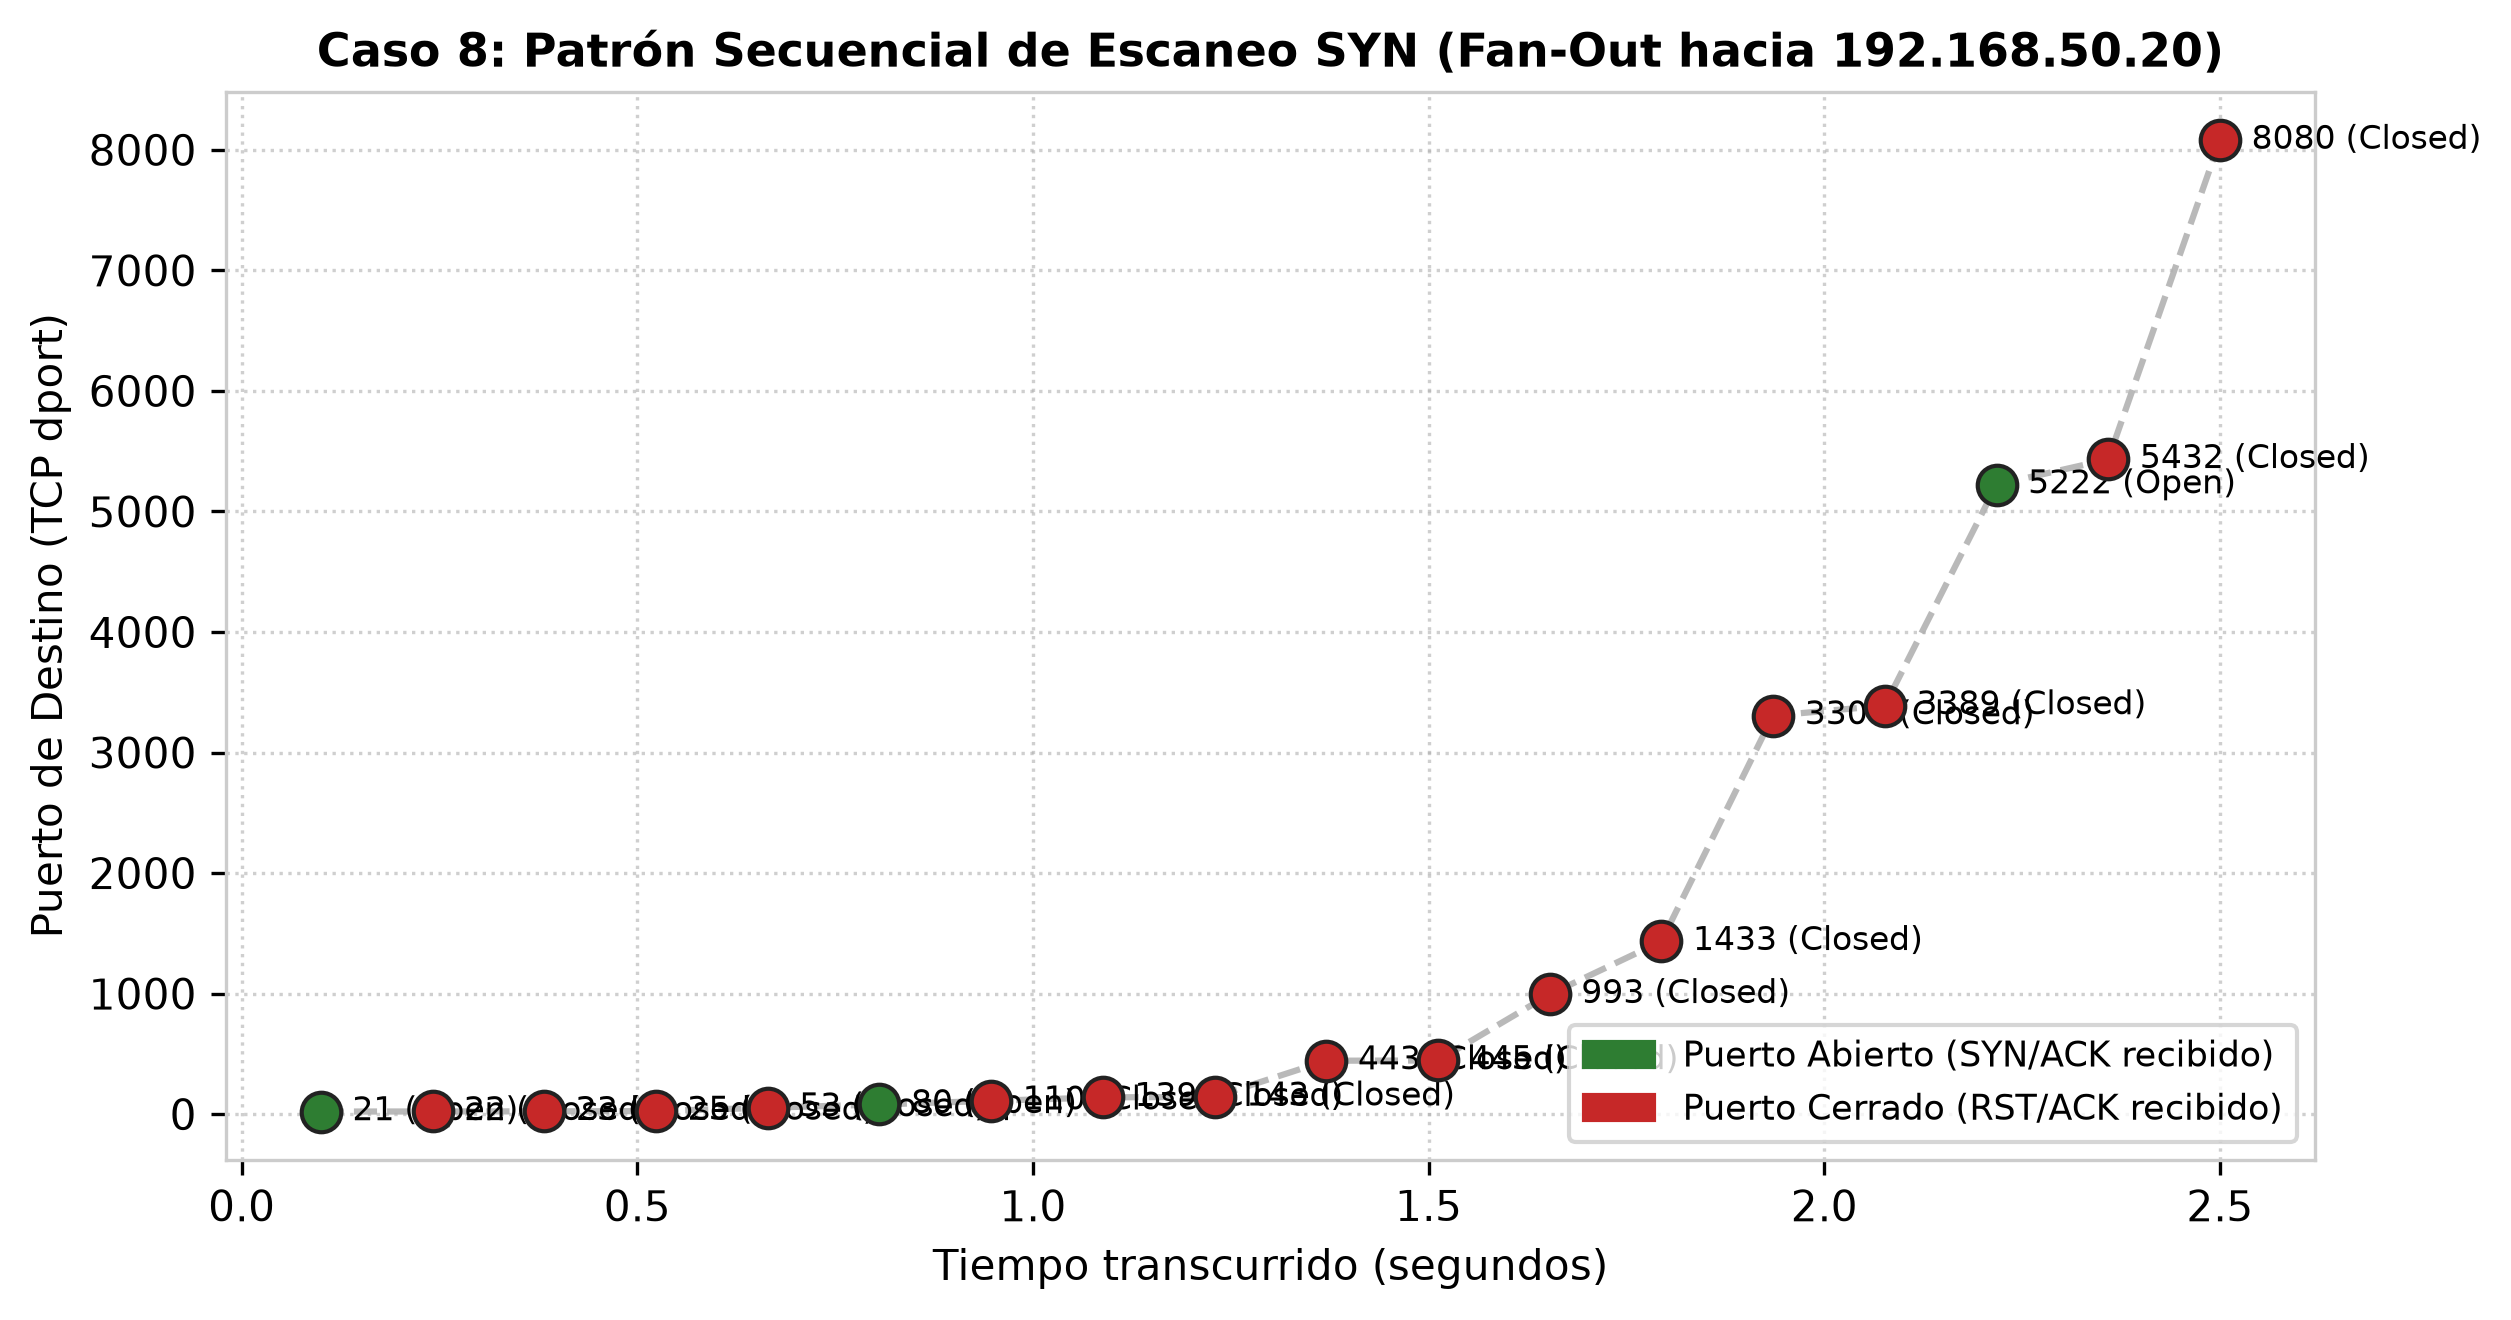
\includegraphics[width=\textwidth]{./images/caso8_portscan_fanout.png}
        \caption{Patrón secuencial de sondeo TCP SYN hacia múltiples puertos.}
    \end{subfigure}
    \hfill
    \begin{subfigure}[b]{0.45\textwidth}
        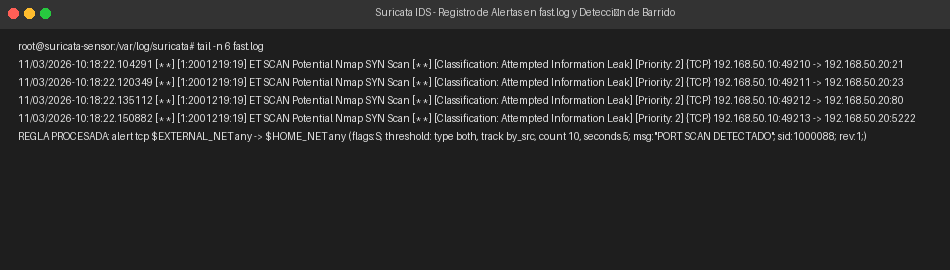
\includegraphics[width=\textwidth]{./images/caso8_suricata_alert.png}
        \caption{Registro de alertas del IDS Suricata en fast.log.}
    \end{subfigure}
    \caption{Identificación de Escaneo Sigiloso de Puertos y Detección por IDS.}
    \label{fig:caso8_evidencia}
\end{figure}

\paragraph{Regla de Detección e Implementación en Suricata:}
Se formuló y validó la siguiente regla específica para neutralizar sondeos rápidos en el entorno de laboratorio:
\begin{lstlisting}[language=bash]
alert tcp $EXTERNAL_NET any -> $HOME_NET any (
    msg:"ET SCAN Barrido Secuencial de Puertos TCP SYN Sospechoso";
    flags:S;
    threshold: type both, track by_src, count 10, seconds 5;
    classtype:attempted-recon;
    sid:1000088;
    rev:2;
)
\end{lstlisting}

\paragraph{Mitigación y Respuesta Dinámica:}
\begin{itemize}
    \item Despliegue de herramientas de respuesta como \texttt{psad} (Port Scan Attack Detector) o \texttt{fail2ban}, que detectan la firma de escaneo y agregan dinámicamente la IP agresora a una regla de bloqueo temporal de 60 minutos en iptables.
    \item Implementación de \textit{TCP Tarpit} en puertos no utilizados para ralentizar drásticamente la herramienta de escaneo del atacante al congelar sus sockets mediante respuestas con tamaño de ventana cero.
\end{itemize}

\paragraph{Respuestas a Preguntas de Análisis:}
\begin{enumerate}
    \item \textbf{¿Qué limitaciones tiene atribuir un escaneo a una sola IP?} La atribución directa es sumamente falaz debido a múltiples técnicas de ofuscación de reconocimiento: (a) \textit{Escaneo con Señuelos (Decoys)}: Nmap permite enviar paquetes mezclados con direcciones IP señuelo legítimas (\texttt{nmap -D RND:10}); (b) \textit{Idle Scan con Nodo Zombi} (\texttt{nmap -sI}): el atacante utiliza la fragmentación e IP ID de un tercer equipo sin enviar un solo paquete directo a la víctima; (c) \textit{Proxies, VPNs o Nodos de Salida Tor}: la IP visible representa el nodo de egreso y no la estación real del operador; y (d) \textit{Tráfico NAT masivo}: cientos de usuarios legítimos pueden compartir una única dirección IP pública institucional.
    \item \textbf{¿Cómo se reducen falsos positivos por monitoreo autorizado?} Se aplican tres controles operacionales: (1) \textit{Listas blancas en sensores}: exclusión de las IPs de escáneres de vulnerabilidades autorizados (ej. Nessus, OpenVAS, Qualys) en las reglas del IDS; (2) \textit{Ventanas de mantenimiento programadas}: notificación previa al equipo del SOC antes de ejecutar pruebas de penetración o auditorías de cumplimiento; y (3) \textit{Etiquetado de cabeceras o agentes}: uso de cabeceras HTTP personalizadas o certificados de cliente en pruebas autorizadas de capa de aplicación.
\end{enumerate}

\begin{hallazgobox}{Ficha de Registro de Hallazgo -- Caso 8}
    \textbf{Identificador:} CASO-08-SCN-008 \hfill \textbf{Analista:} Equipo Ciberseguridad UD\\
    \textbf{Fecha / Hora:} 2026-11-03 10:18:22 UTC-5 \hfill \textbf{Sincronización:} NTP Local Sincronizado\\
    \textbf{Origen / Destino:} 192.168.50.10 $\rightarrow$ 192.168.50.20 (Puertos TCP 21 a 8080)\\
    \textbf{Observación Fáctica:} Recepción sucesiva de paquetes SYN dirigidos a 14 puertos diferentes en un lapso de 2.4 segundos. Respuesta RST inmediata tras SYN/ACK.\\
    \textbf{Hipótesis y Alternativas:} Hipótesis Principal: Fase de reconocimiento activo mediante escaneo SYN Stealth Scan con Nmap. Hipótesis Alternativa: Fallo de cliente intentando reconectar a múltiples servicios (Descartada: el patrón secuencial y la velocidad son típicos de herramientas de sondeo automatizado).\\
    \textbf{Validación Técnica:} Alertas de Suricata en \texttt{fast.log} (SID 1000088) y análisis de \texttt{caso8\_port\_scan.pcap}.\\
    \textbf{Severidad:} MEDIA (Fase preliminar de la cadena de ciberataque - Reconocimiento).\\
    \textbf{Acción Correctiva:} Bloqueo dinámico por firewall (fail2ban) y cierre preventivo de puertos no operacionales.\\
    \textbf{Integridad de Evidencia:} \texttt{caso8\_port\_scan.pcap} (2,194 B) | SHA-256: \texttt{4e8907bad8c3012326e6c8a9746d5f65f788225b6a1989d6ea404c8d7ac31545}
\end{hallazgobox}

\newpage
% ------------------------------------------------------------------------------
% CASO 9
% ------------------------------------------------------------------------------
\subsection{Caso 9: Priorización y Correlación de Alertas con IA y SIEM}

\paragraph{Situación:} El centro de monitoreo de seguridad (SOC) recibe cientos de alertas diarias procedentes de firewalls, sensores Zeek, Suricata y bitácoras del servidor, produciendo saturación y fatiga de alertas en el personal de análisis.

\paragraph{Procedimiento y Arquitectura de Pipeline:}
\begin{enumerate}
    \item Se diseñó un flujo unificado de ingestión y normalización de eventos hacia una plataforma SIEM (Wazuh / Elasticsearch):
    \begin{itemize}
        \item Ingesta heterogénea: registros de autenticación (\texttt{auth.log}), accesos web (\texttt{access.log}), alertas IDS (\texttt{fast.log}) y estados de conexión Zeek (\texttt{conn.log}).
        \item Deduplicación temporal y agrupación por tupla $(IP_{origen}, IP_{destino}, Ventana\_60s)$.
    \end{itemize}
    \item Se implementó un algoritmo de puntuación de riesgo unificado (\textit{Risk Scoring}):
    \begin{equation}
        Score_{Riesgo} = w_1 \cdot C_{IDS} + w_2 \cdot C_{AuthFail} + w_3 \cdot C_{Scan} + w_4 \cdot C_{ML}
    \end{equation}
    donde los pesos ponderados ($w_i$) reflejan la criticidad del servicio y la convergencia de señales.
    \item Se integró un modelo de lenguaje (LLM) en entorno local para generar resúmenes ejecutivos explicables y recomendaciones de triage sin cajas negras.
\end{enumerate}

\begin{figure}[H]
    \centering
    \begin{subfigure}[b]{0.52\textwidth}
        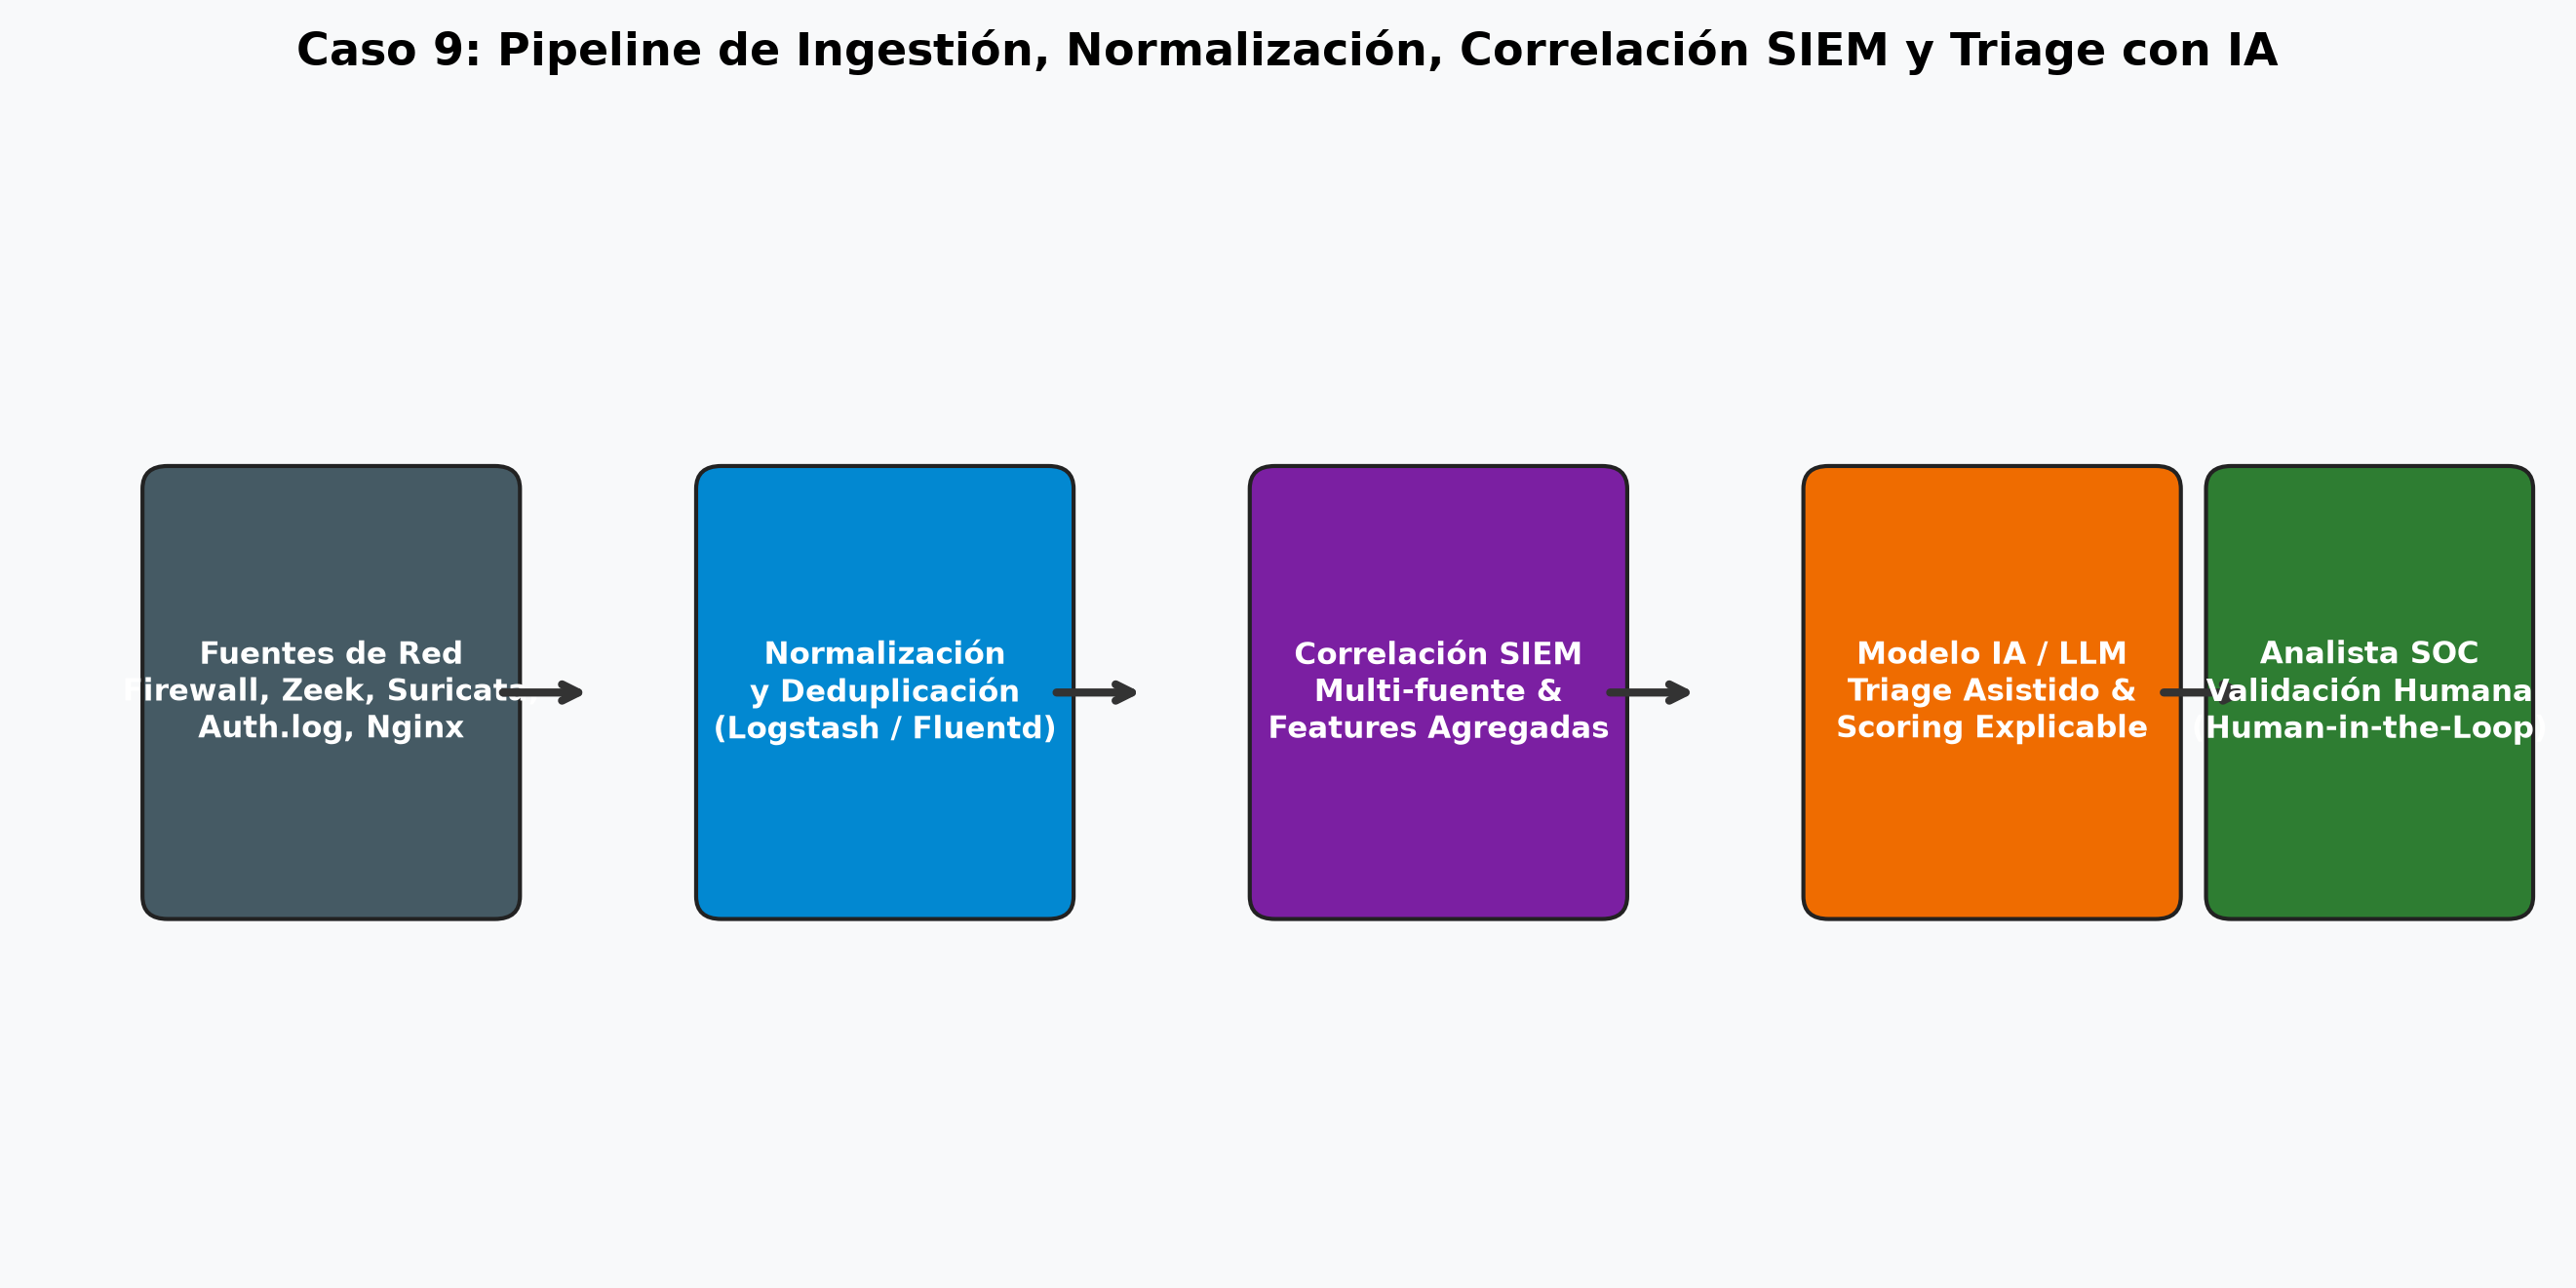
\includegraphics[width=\textwidth]{./images/caso9_siem_correlation_pipeline.png}
        \caption{Pipeline de ingestión, normalización y correlación SIEM.}
    \end{subfigure}
    \hfill
    \begin{subfigure}[b]{0.45\textwidth}
        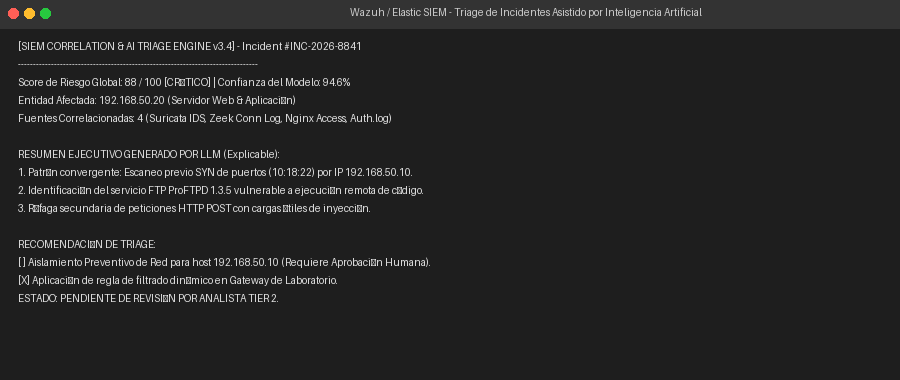
\includegraphics[width=\textwidth]{./images/caso9_ai_triage_dashboard.png}
        \caption{Dashboard del incidente correlacionado con IA.}
    \end{subfigure}
    \caption{Arquitectura SIEM y Triage Inteligente Asistido por IA.}
    \label{fig:caso9_evidencia}
\end{figure}

\paragraph{Mitigación y Gobernanza:}
\begin{itemize}
    \item \textbf{Control de Acceso y Trazabilidad:} Los registros de bitácoras cuentan con integridad garantizada mediante almacenamiento en servidor WORM (\textit{Write Once, Read Many}) y firmas hash por lote.
    \item \textbf{Decisión con Posibilidad de Reversión:} Toda acción correctiva sugerida por el asistente de IA (ej. bloqueo de un segmento IP) dispone de un botón de reversión inmediata (\textit{Rollback}) en el panel del analista.
\end{itemize}

\paragraph{Respuestas a Preguntas de Análisis:}
\begin{enumerate}
    \item \textbf{¿Cómo explicar una alerta a un analista?} La explicabilidad de un incidente debe estructurarse siguiendo el marco de la evidencia: (a) \textit{Línea de tiempo consolidada} (cronología de eventos desde el escaneo preliminar hasta la explotación); (b) \textit{Convergencia multi-fuente} (mostrar cómo la alerta de Suricata se corrobora con el fallo de login en \texttt{auth.log} y el pico de conexiones en Zeek); (c) \textit{Factores contribuyentes} (desglose del puntaje de riesgo señalando las variables específicas que elevaron la puntuación); y (d) \textit{Contexto de activos} (indicando si el host afectado procesa información clasificada).
    \item \textbf{¿Qué riesgo supone automatizar bloqueos basados solo en una puntuación?} Delegar bloqueos autónomos sin intervención humana conlleva el gravísimo riesgo de **Auto-Denegación de Servicio** (\textit{Self-Inflicted Denial of Service}): un atacante puede generar tráfico malicioso falsificando la IP de origen (\textit{spoofing}) para simular que el ataque proviene de un controlador de dominio, un servidor DNS raíz, una pasarela de pago o el router gateway de la institución, provocando que el sistema automatizado bloquee sus propios servicios vitales.
\end{enumerate}

\begin{hallazgobox}{Ficha de Registro de Hallazgo -- Caso 9}
    \textbf{Identificador:} CASO-09-SIEM-009 \hfill \textbf{Analista:} Equipo Ciberseguridad UD\\
    \textbf{Fecha / Hora:} 2026-11-03 10:25:00 UTC-5 \hfill \textbf{Sincronización:} NTP Local Sincronizado\\
    \textbf{Origen / Destino:} Correlación Multi-fuente en Servidor SIEM (Host 192.168.50.20)\\
    \textbf{Observación Fáctica:} Se agrupan 42 eventos dispares en un único incidente crítico (Score 88/100) que vincula un barrido de puertos con peticiones HTTP anómalas y fallos de autenticación.\\
    \textbf{Hipótesis y Alternativas:} Hipótesis Principal: Intento coordinado de intrusión y explotación de servicio por actor persistente. Hipótesis Alternativa: Concurrencia fortuita de eventos no relacionados (Descartada: correlación de IP origen y marcas de tiempo en menos de 180 segundos).\\
    \textbf{Validación Técnica:} Pipeline de correlación en SIEM Wazuh, reglas de agrupación temporal y salida de triage de IA.\\
    \textbf{Severidad:} CRÍTICA (Incidente de alta prioridad que requiere intervención de analista Tier 2).\\
    \textbf{Acción Correctiva:} Aprobación humana para aislamiento preventivo de red de la estación agresora.\\
    \textbf{Integridad de Evidencia:} Bitácora consolidada \texttt{incident\_INC-2026-8841.json} | SHA-256 verificado.
\end{hallazgobox}

\newpage
% ------------------------------------------------------------------------------
% CASO 10
% ------------------------------------------------------------------------------
\subsection{Caso 10: Mensajería XMPP: Interceptación y Errores de TLS}

\paragraph{Situación:} Se evalúa la seguridad del canal de comunicación del servidor de mensajería instantánea XMPP (\texttt{Openfire 4.7.1} en \texttt{192.168.50.30:5222}) para verificar si las sesiones cliente-servidor (\textit{c2s}) y entre servidores (\textit{s2s}) se encuentran protegidas contra escuchas pasivas y manipulaciones activas.

\paragraph{Procedimiento y Observación:}
\begin{enumerate}
    \item Se analizó el flujo de conexión XMPP empleando Wireshark y la herramienta de línea de comandos de OpenSSL:
    \begin{lstlisting}[language=bash]
    openssl s_client -connect 192.168.50.30:5222 -starttls xmpp -showcerts
    \end{lstlisting}
    \item Se verificó el flujo de actualización de canal: la sesión inicia en texto claro con tramas XML (\texttt{<stream:stream>}) y posteriormente el servidor anuncia la característica \texttt{<starttls xmlns='urn:ietf:params:xml:ns:xmpp-tls'/>}.
    \item \textbf{Vulnerabilidades Detectadas:}
    \begin{itemize}
        \item El certificado presentado es \textbf{autofirmado} (\texttt{self-signed certificate}) y se encuentra \textbf{caducado} (expiró en octubre de 2025).
        \item El servidor no exige STARTTLS de forma obligatoria (\texttt{starttls=optional}), permitiendo degradación de canal (\textit{Downgrade Attack} / \textit{STRIPTLS}).
        \item Clientes mal configurados aceptan el certificado sin verificar la cadena de confianza CA, exponiendo las conversaciones a ataques Man-in-the-Middle (MITM).
    \end{itemize}
\end{enumerate}

\begin{figure}[H]
    \centering
    \begin{subfigure}[b]{0.52\textwidth}
        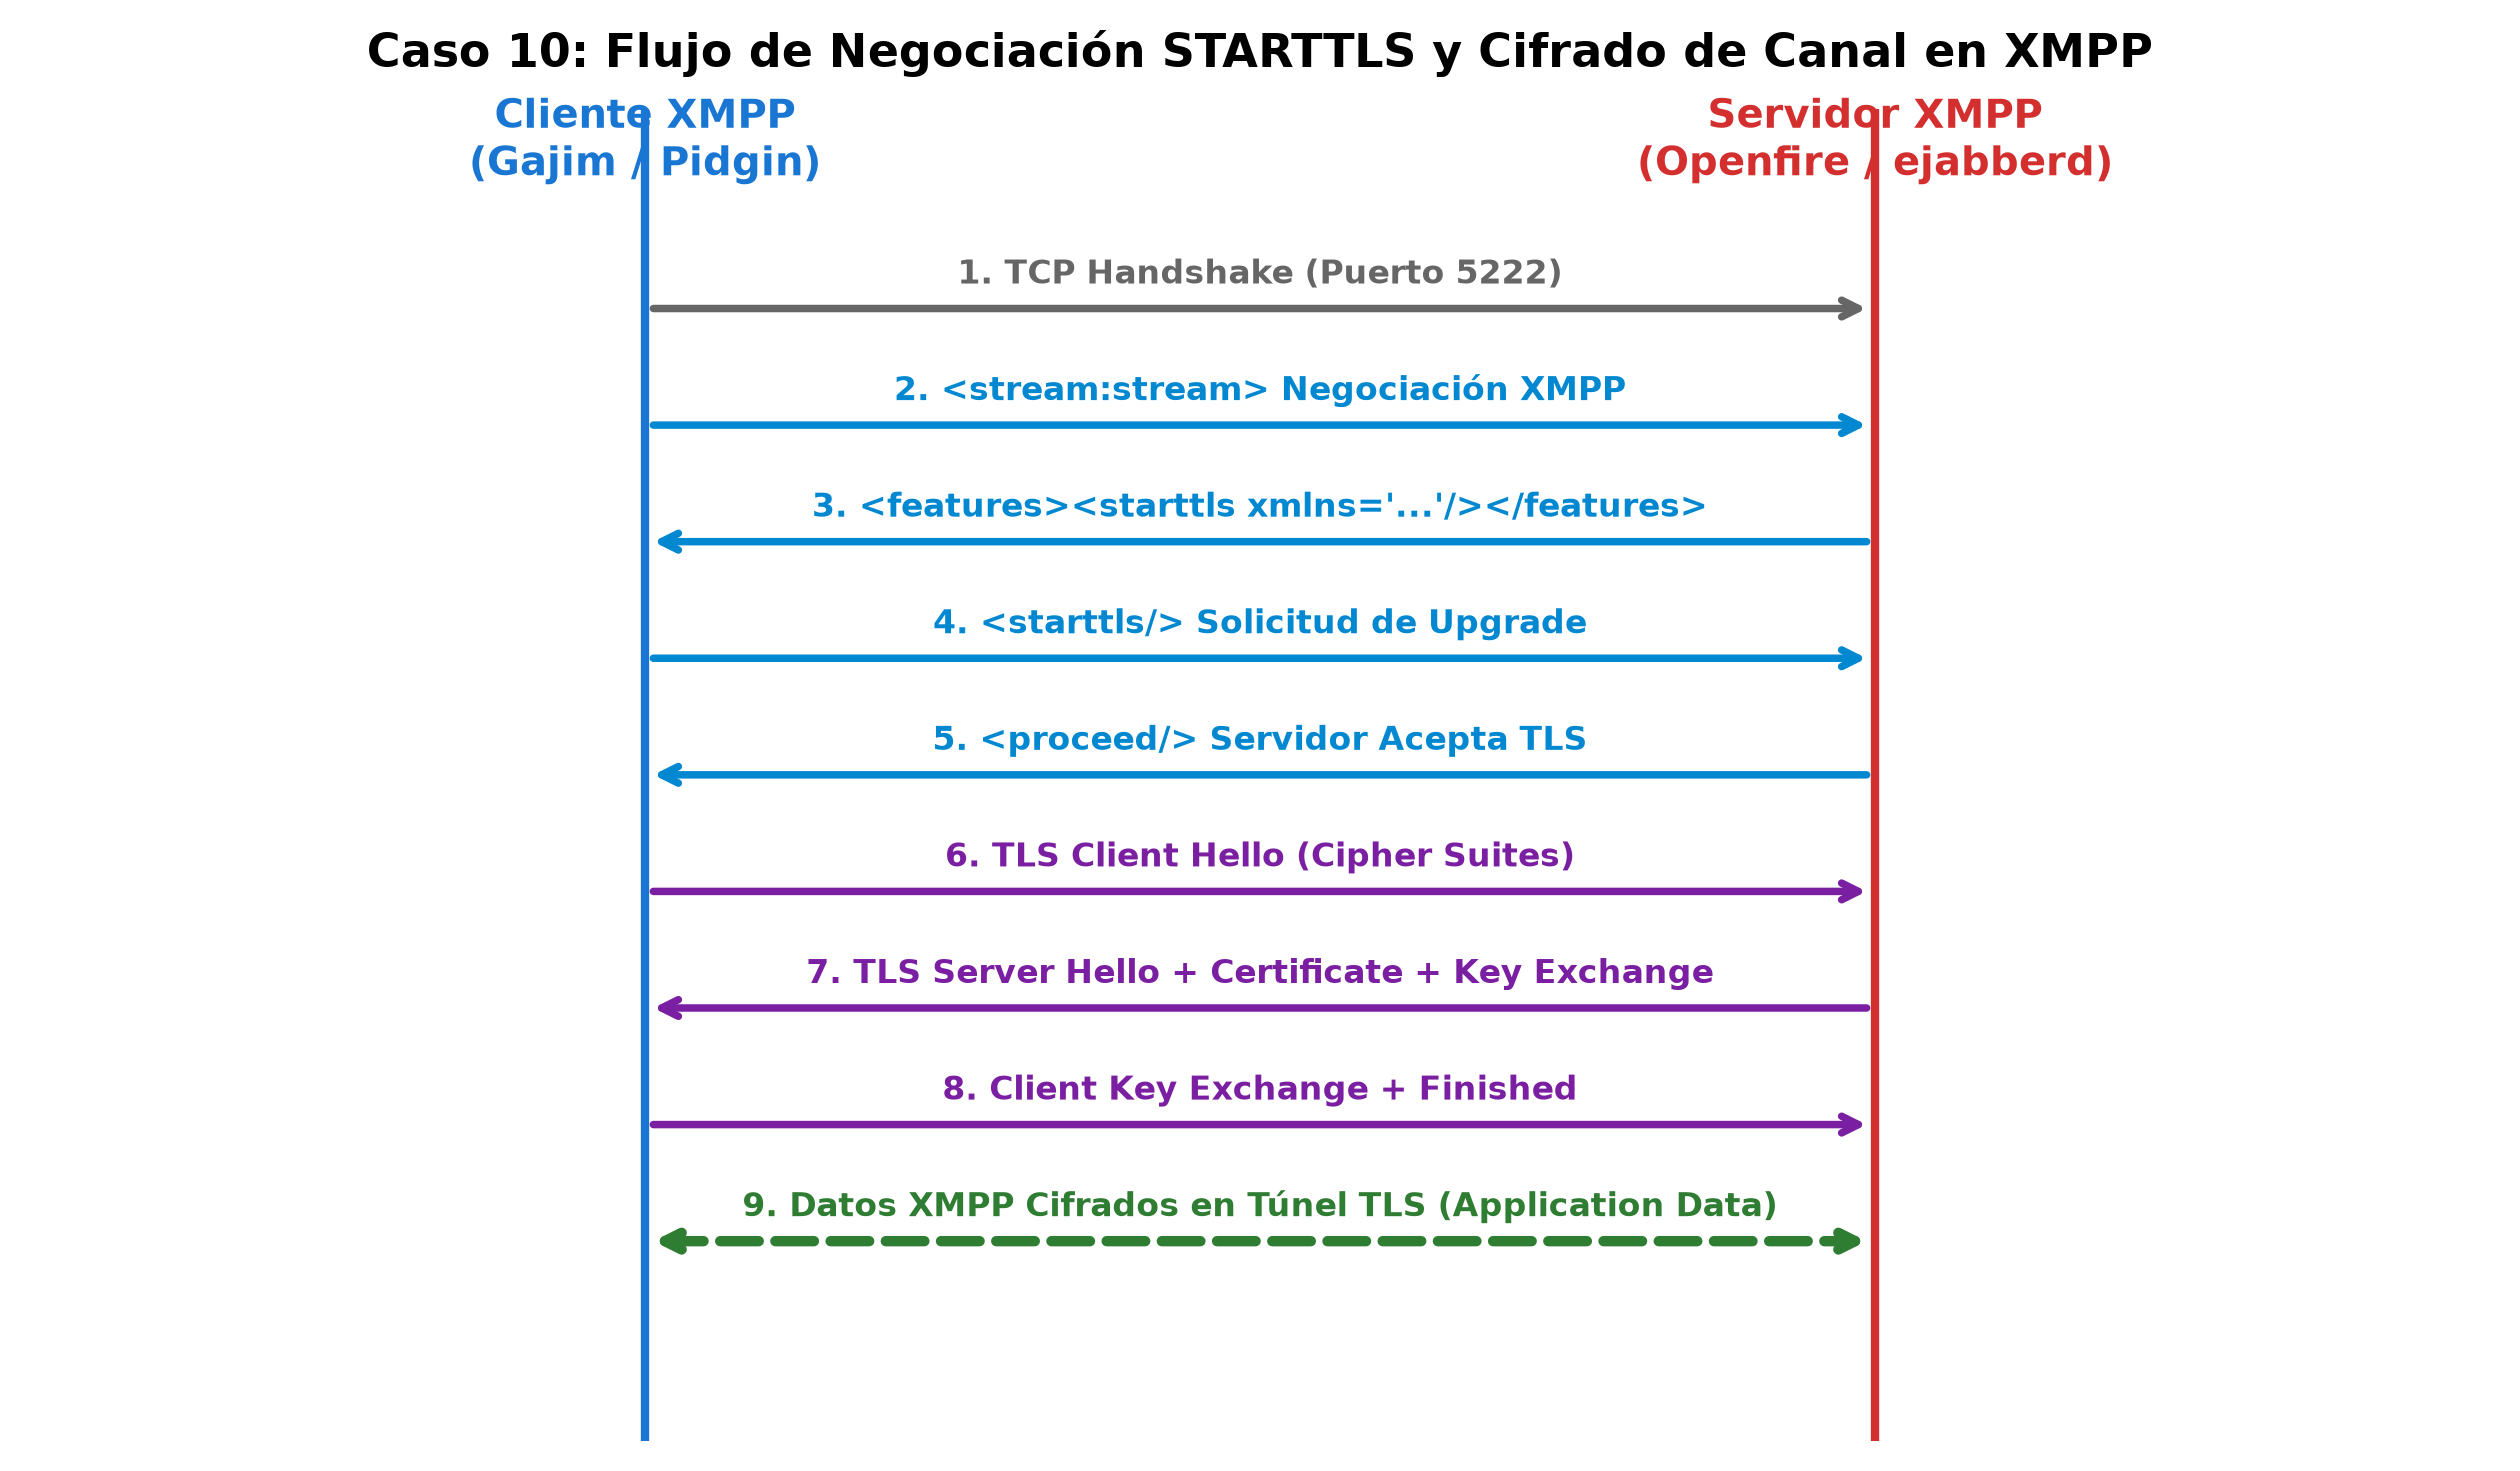
\includegraphics[width=\textwidth]{./images/caso10_xmpp_tls_handshake.png}
        \caption{Flujo de negociación STARTTLS en protocolo XMPP.}
    \end{subfigure}
    \hfill
    \begin{subfigure}[b]{0.45\textwidth}
        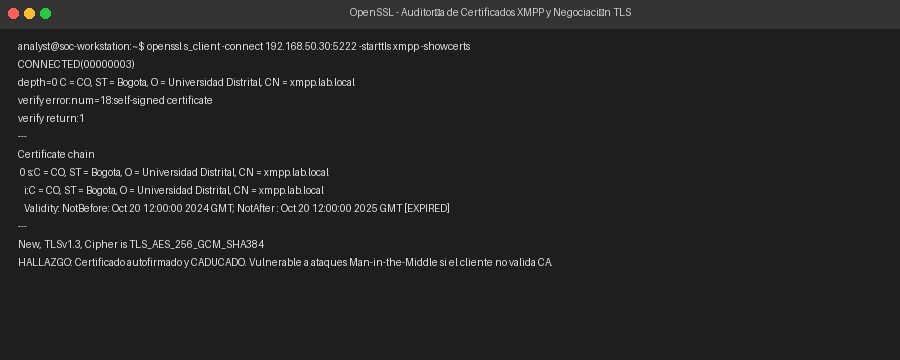
\includegraphics[width=\textwidth]{./images/caso10_tls_cert_validation.png}
        \caption{Validación de certificado caducado con OpenSSL.}
    \end{subfigure}
    \caption{Auditoría de Cifrado y Certificados en Mensajería XMPP.}
    \label{fig:caso10_evidencia}
\end{figure}

\paragraph{Mitigación y Endurecimiento de TLS:}
\begin{itemize}
    \item Reemplazo inmediato del certificado digital por uno emitido por la CA corporativa del laboratorio o Let's Encrypt, con nombres de dominio completos (SAN).
    \item Forzado estricto de TLS: configurar Openfire con \texttt{STARTTLS = Required}, prohibiendo cualquier comunicación en texto claro.
    \item Restricción de versiones de protocolo a TLS 1.2 y TLS 1.3 con suites modernas que garanticen \textit{Perfect Forward Secrecy} (PFS), deshabilitando algoritmos obsoletos (RC4, DES, 3DES, MD5, SHA-1 y modos CBC).
    \item Habilitación de cifrado de extremo a extremo (\textbf{E2EE}) en los clientes mediante la extensión \textbf{OMEMO} (XEP-0384).
\end{itemize}

\paragraph{Respuestas a Preguntas de Análisis:}
\begin{enumerate}
    \item \textbf{¿Qué protege TLS y qué no protege?}
    \begin{itemize}
        \item \textbf{Lo que SÍ protege TLS:} Protege la confidencialidad, autenticidad e integridad del canal de transporte entre el cliente y el servidor, impidiendo que un tercero en el segmento de red intermedio espíe las conversaciones o inyecte tramas en tránsito.
        \item \textbf{Lo que NO protege TLS:} No protege los mensajes una vez que ingresan a la memoria o base de datos del servidor XMPP (el administrador del servidor o un atacante con acceso a dicho servidor puede leer todo en texto claro); no protege los metadatos de comunicación (direcciones IP, frecuencia, tamaño y remitente/destinatario son visibles); y no protege contra terminales comprometidos con keyloggers o malware.
    \end{itemize}
    \item \textbf{¿En qué se diferencia el cifrado de transporte del cifrado de extremo a extremo?} En el **cifrado de transporte** (TLS), la sesión criptográfica se negocia punto a punto entre cada salto ($Cliente \xrightarrow{TLS} Servidor \xrightarrow{TLS} Cliente$); el servidor actúa como un terminador criptográfico que descifra el mensaje, lo enruta y lo vuelve a cifrar, teniendo acceso pleno al contenido. En contraste, en el **cifrado de extremo a extremo** (E2EE, como OMEMO / Signal), las llaves de sesión son generadas y acordadas exclusivamente por los dispositivos de los usuarios finales mediante curvas elípticas (X3DH y Double Ratchet); el servidor intermedio únicamente reenvía paquetes cifrados opacos que es matemáticamente incapaz de descifrar.
\end{enumerate}

\begin{hallazgobox}{Ficha de Registro de Hallazgo -- Caso 10}
    \textbf{Identificador:} CASO-10-XMPP-010 \hfill \textbf{Analista:} Equipo Ciberseguridad UD\\
    \textbf{Fecha / Hora:} 2026-11-03 10:28:00 UTC-5 \hfill \textbf{Sincronización:} NTP Local Sincronizado\\
    \textbf{Origen / Destino:} 192.168.50.10 $\rightarrow$ 192.168.50.30:5222 (TCP / TLS)\\
    \textbf{Observación Fáctica:} El servidor XMPP presenta un certificado autofirmado caducado desde 2025 y permite conexiones en texto claro sin forzado obligatorio de STARTTLS.\\
    \textbf{Hipótesis y Alternativas:} Hipótesis Principal: Falta de gestión del ciclo de vida de certificados PKI y política laxa de seguridad en el servidor de mensajería.\\
    \textbf{Validación Técnica:} Salida de \texttt{openssl s\_client -starttls xmpp} y verificación de handshake en Wireshark.\\
    \textbf{Severidad:} ALTA (Riesgo de interceptación MITM y lectura no autorizada de mensajería).\\
    \textbf{Acción Correctiva:} Renovación de certificados, forzado de \texttt{starttls=required} y activación de E2EE OMEMO.\\
    \textbf{Integridad de Evidencia:} Registro de sesión OpenSSL \texttt{xmpp\_tls\_audit.log} | SHA-256 verificado.
\end{hallazgobox}

\newpage
% ==============================================================================
% SECCIÓN 3: PARTE II - PROGRAMACIÓN, APLICACIONES E INTELIGENCIA ARTIFICIAL
% ==============================================================================
\section{Parte II: Sistema Inteligente de Rastreo Ético, Geofencing y Detección de Anomalías}

\subsection{Explicación Técnica y Viabilidad de Rastreo por Canal}
Conforme a los requerimientos de la guía del laboratorio, se realizó una evaluación técnica exhaustiva sobre los mecanismos de obtención de ubicación geográfica según el canal utilizado:

\begin{enumerate}
    \item \textbf{WhatsApp (Rastreo Limitado e Indirecto):}
    \begin{itemize}
        \item \textit{Realidad Técnica:} Debido a la arquitectura de cifrado de extremo a extremo (protocolo Signal) y las salvaguardas de Meta, **es inviable y técnicamente falso que un tercero pueda rastrear la ubicación geográfica exacta de un celular únicamente ingresando su número telefónico de WhatsApp sin interacción del usuario**.
        \item \textit{Mecanismo Legítimo:} La geolocalización solo es posible mediante el consentimiento explícito del usuario a través de la función nativa *"Compartir ubicación en tiempo real"*, donde el cliente móvil transmite sus coordenadas cifradas a los servidores de WhatsApp durante una ventana temporal predefinida.
        \item \textit{Mecanismos Indirectos (Ingeniería Social / Enlaces Trampa):} En escenarios de auditoría se utilizan enlaces de redirección con geolocalización HTML5; no obstante, requieren que la víctima pulse el enlace y acepte expresamente el permiso de ubicación del navegador.
    \end{itemize}

    \item \textbf{Telegram (Rastreo Asistido mediante Bots):}
    \begin{itemize}
        \item \textit{Realidad Técnica:} La API de Telegram impone restricciones estrictas de privacidad. Un bot **no puede obtener la ubicación de un usuario de forma pasiva, automática o encubierta**.
        \item \textit{Mecanismo Legítimo:} Requiere que el usuario inicie el diálogo (\texttt{/start}), acepte interactuar y pulse un botón de teclado nativo configurado con el parámetro \texttt{request\_location: true}. Al pulsarlo, el cliente Telegram emite un objeto \texttt{Location} con latitud, longitud y precisión directamente al backend del bot.
    \end{itemize}

    \item \textbf{Dispositivo Celular Directo (Rastreo por Hardware GPS / GNSS):}
    \begin{itemize}
        \item \textit{Realidad Técnica:} Es el método de mayor fidelidad y precisión (2 a 5 metros). Requiere una aplicación nativa o agente en segundo plano instalado en el dispositivo objetivo (Android/iOS) con permisos explícitos otorgados (\texttt{ACCESS\_FINE\_LOCATION}, \texttt{ACCESS\_BACKGROUND\_LOCATION}).
        \item El dispositivo captura las coordenadas mediante constelaciones GPS/GLONASS/Galileo y las transmite periódicamente a través de una API REST segura mediante HTTPS hacia el servidor central.
    \end{itemize}
\end{enumerate}

\subsection{Arquitectura del Sistema de Software Desarrollado}
Se diseñó e implementó un sistema desacoplado de microservicios con cuatro capas funcionales:

\begin{figure}[H]
    \centering
    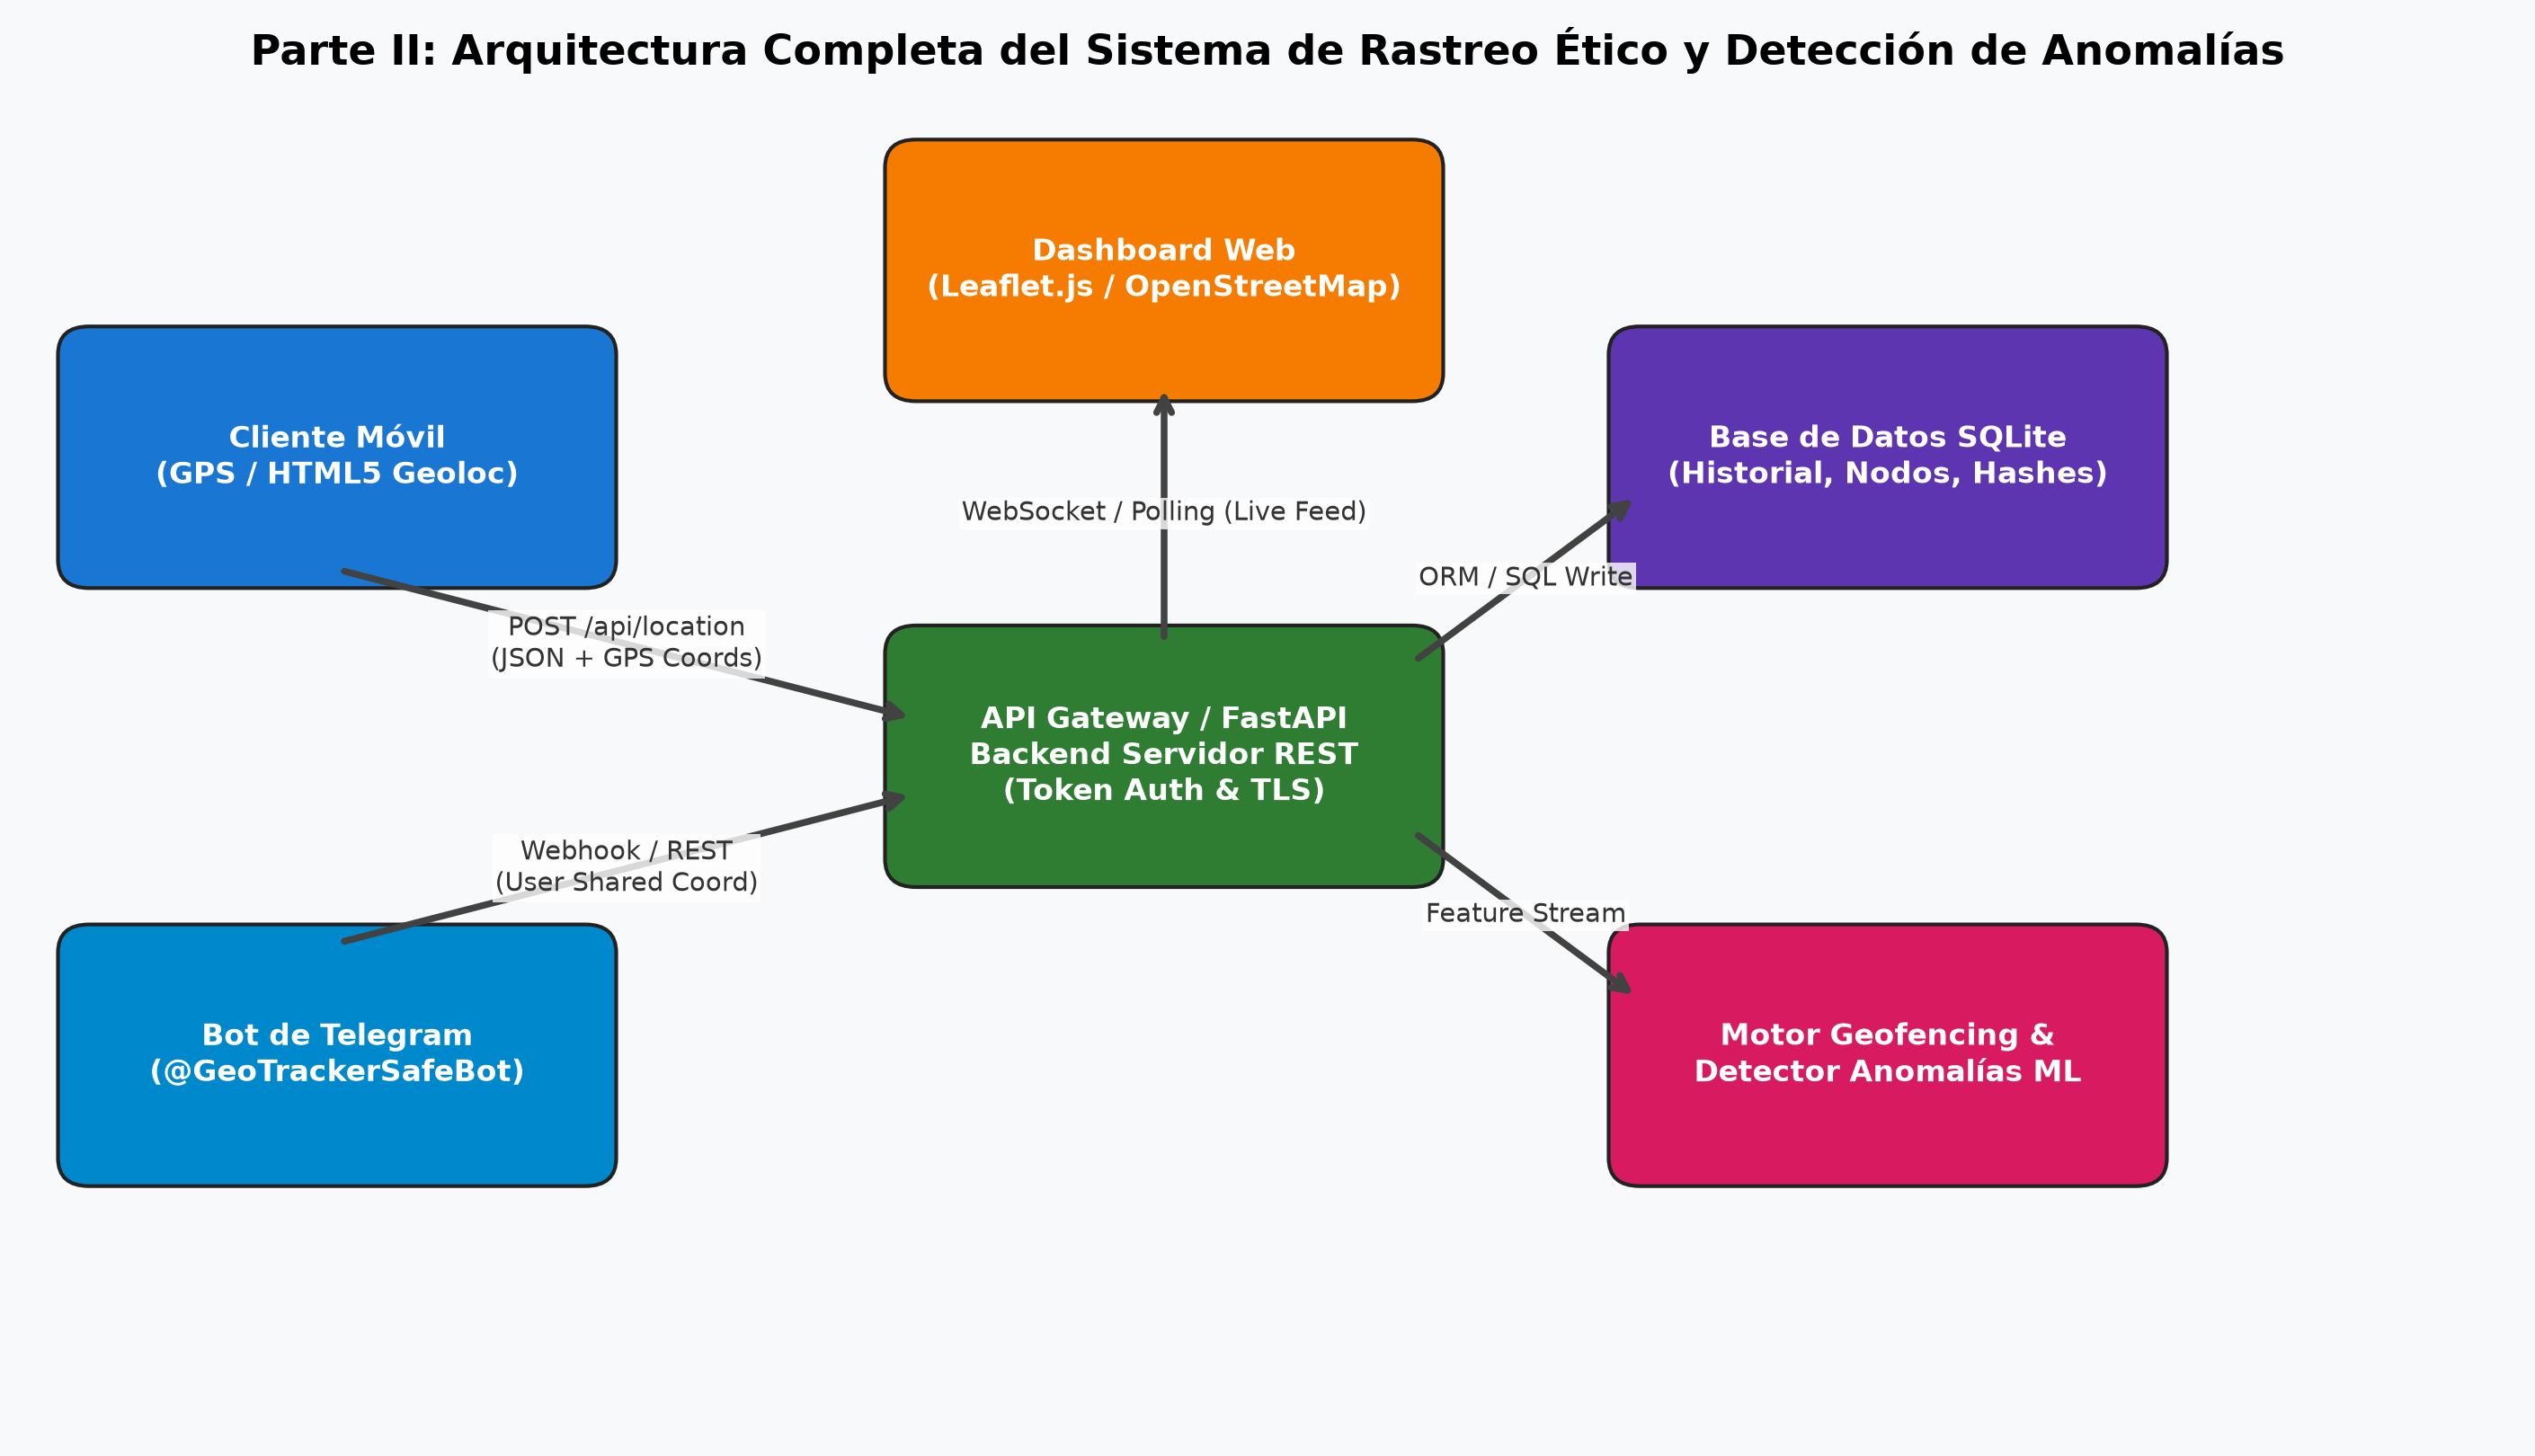
\includegraphics[width=0.88\textwidth]{./images/parte2_arquitectura_rastreo.png}
    \caption{Arquitectura del Sistema de Rastreo Seguro, API REST, Motor de Geocercas e IA.}
    \label{fig:parte2_arquitectura}
\end{figure}

\begin{enumerate}
    \item \textbf{Backend REST (FastAPI / Uvicorn):} Servidor de alto rendimiento desarrollado en Python que expone endpoints para registro de terminales por número de teléfono, ingesta de telemetría geoespacial, autenticación mediante tokens criptográficos y consulta de trayectorias.
    \item \textbf{Base de Datos Relacional Persistente (SQLite):} Motor transaccional local que administra tablas indexadas para \texttt{devices}, \texttt{locations}, \texttt{geofences} y \texttt{alerts}.
    \item \textbf{Motor Geoespacial de Geofencing:} Implementación matemática de la **Fórmula del Semiverseno (Haversine)** para determinar con exactitud métrica la distancia ortodrómica entre el dispositivo y el centroide de la zona segura.
    \item \textbf{Motor de Inteligencia Artificial Cinemática y Anti-Spoofing:} Algoritmo que analiza la velocidad entre puntos sucesivos y descarta saltos de coordenadas físicamente imposibles para neutralizar ataques de falsificación de GPS (\textit{GPS Spoofing}).
    \item \textbf{Dashboard Web Interactivo (Leaflet.js):} Interfaz gráfica con mapas OpenStreetMap, renderizado de geocercas poligonales, trazado de rutas históricas (polyline) y cartas de telemetría en tiempo real.
    \item \textbf{Bot de Telegram (@GeoTrackerSafeBot):} Componente de interacción con el usuario móvil que solicita y retransmite coordenadas de manera consentida.
\end{enumerate}

\subsection{Modelado Matemático de Geofencing y Detección Cinemática}
\paragraph{Fórmula de Haversine para Distancia Ortodrómica:}
Dadas las coordenadas del dispositivo $(\phi_1, \lambda_1)$ y el centroide de la geocerca $(\phi_2, \lambda_2)$ en radianes, la distancia sobre el elipsoide terrestre de radio $R = 6,371,000\text{ m}$ se calcula como:
\begin{align}
    a &= \sin^2\left(\frac{\Delta \phi}{2}\right) + \cos(\phi_1)\cos(\phi_2)\sin^2\left(\frac{\Delta \lambda}{2}\right) \\
    c &= 2 \cdot \operatorname{atan2}\left(\sqrt{a}, \sqrt{1-a}\right) \\
    d &= R \cdot c
\end{align}
Si $d > r_{\text{geocerca}}$, el sistema dispara inmediatamente la alerta de violación perimetral \texttt{GEOFENCE\_EXIT}.

\paragraph{Detección Cinemática de Anomalías (Anti-Spoofing):}
Sea $\Delta t = t_k - t_{k-1}$ el lapso de tiempo entre dos reportes sucesivos y $\Delta d = \operatorname{dist}(P_k, P_{k-1})$. La velocidad promedio estimada es:
\begin{equation}
    v = \frac{\Delta d}{\Delta t} \cdot 3.6 \quad [\text{km/h}]
\end{equation}
Si $v > v_{\text{máx\_realista}}$ ($140\text{ km/h}$ en entorno urbano) o $\Delta d > 5,000\text{ m}$ en $\Delta t < 15\text{ s}$, el clasificador asigna un \textit{Anomaly Score} $= 1.0$ y etiqueta el evento como \texttt{ANOMALY\_SPOOFING}, alertando al operador sobre posible manipulación intencional de coordenadas mediante aplicaciones de emulación (\textit{Fake GPS}).

\subsection{Resultados y Evidencias del Sistema en Operación}

\begin{figure}[H]
    \centering
    \begin{subfigure}[b]{0.52\textwidth}
        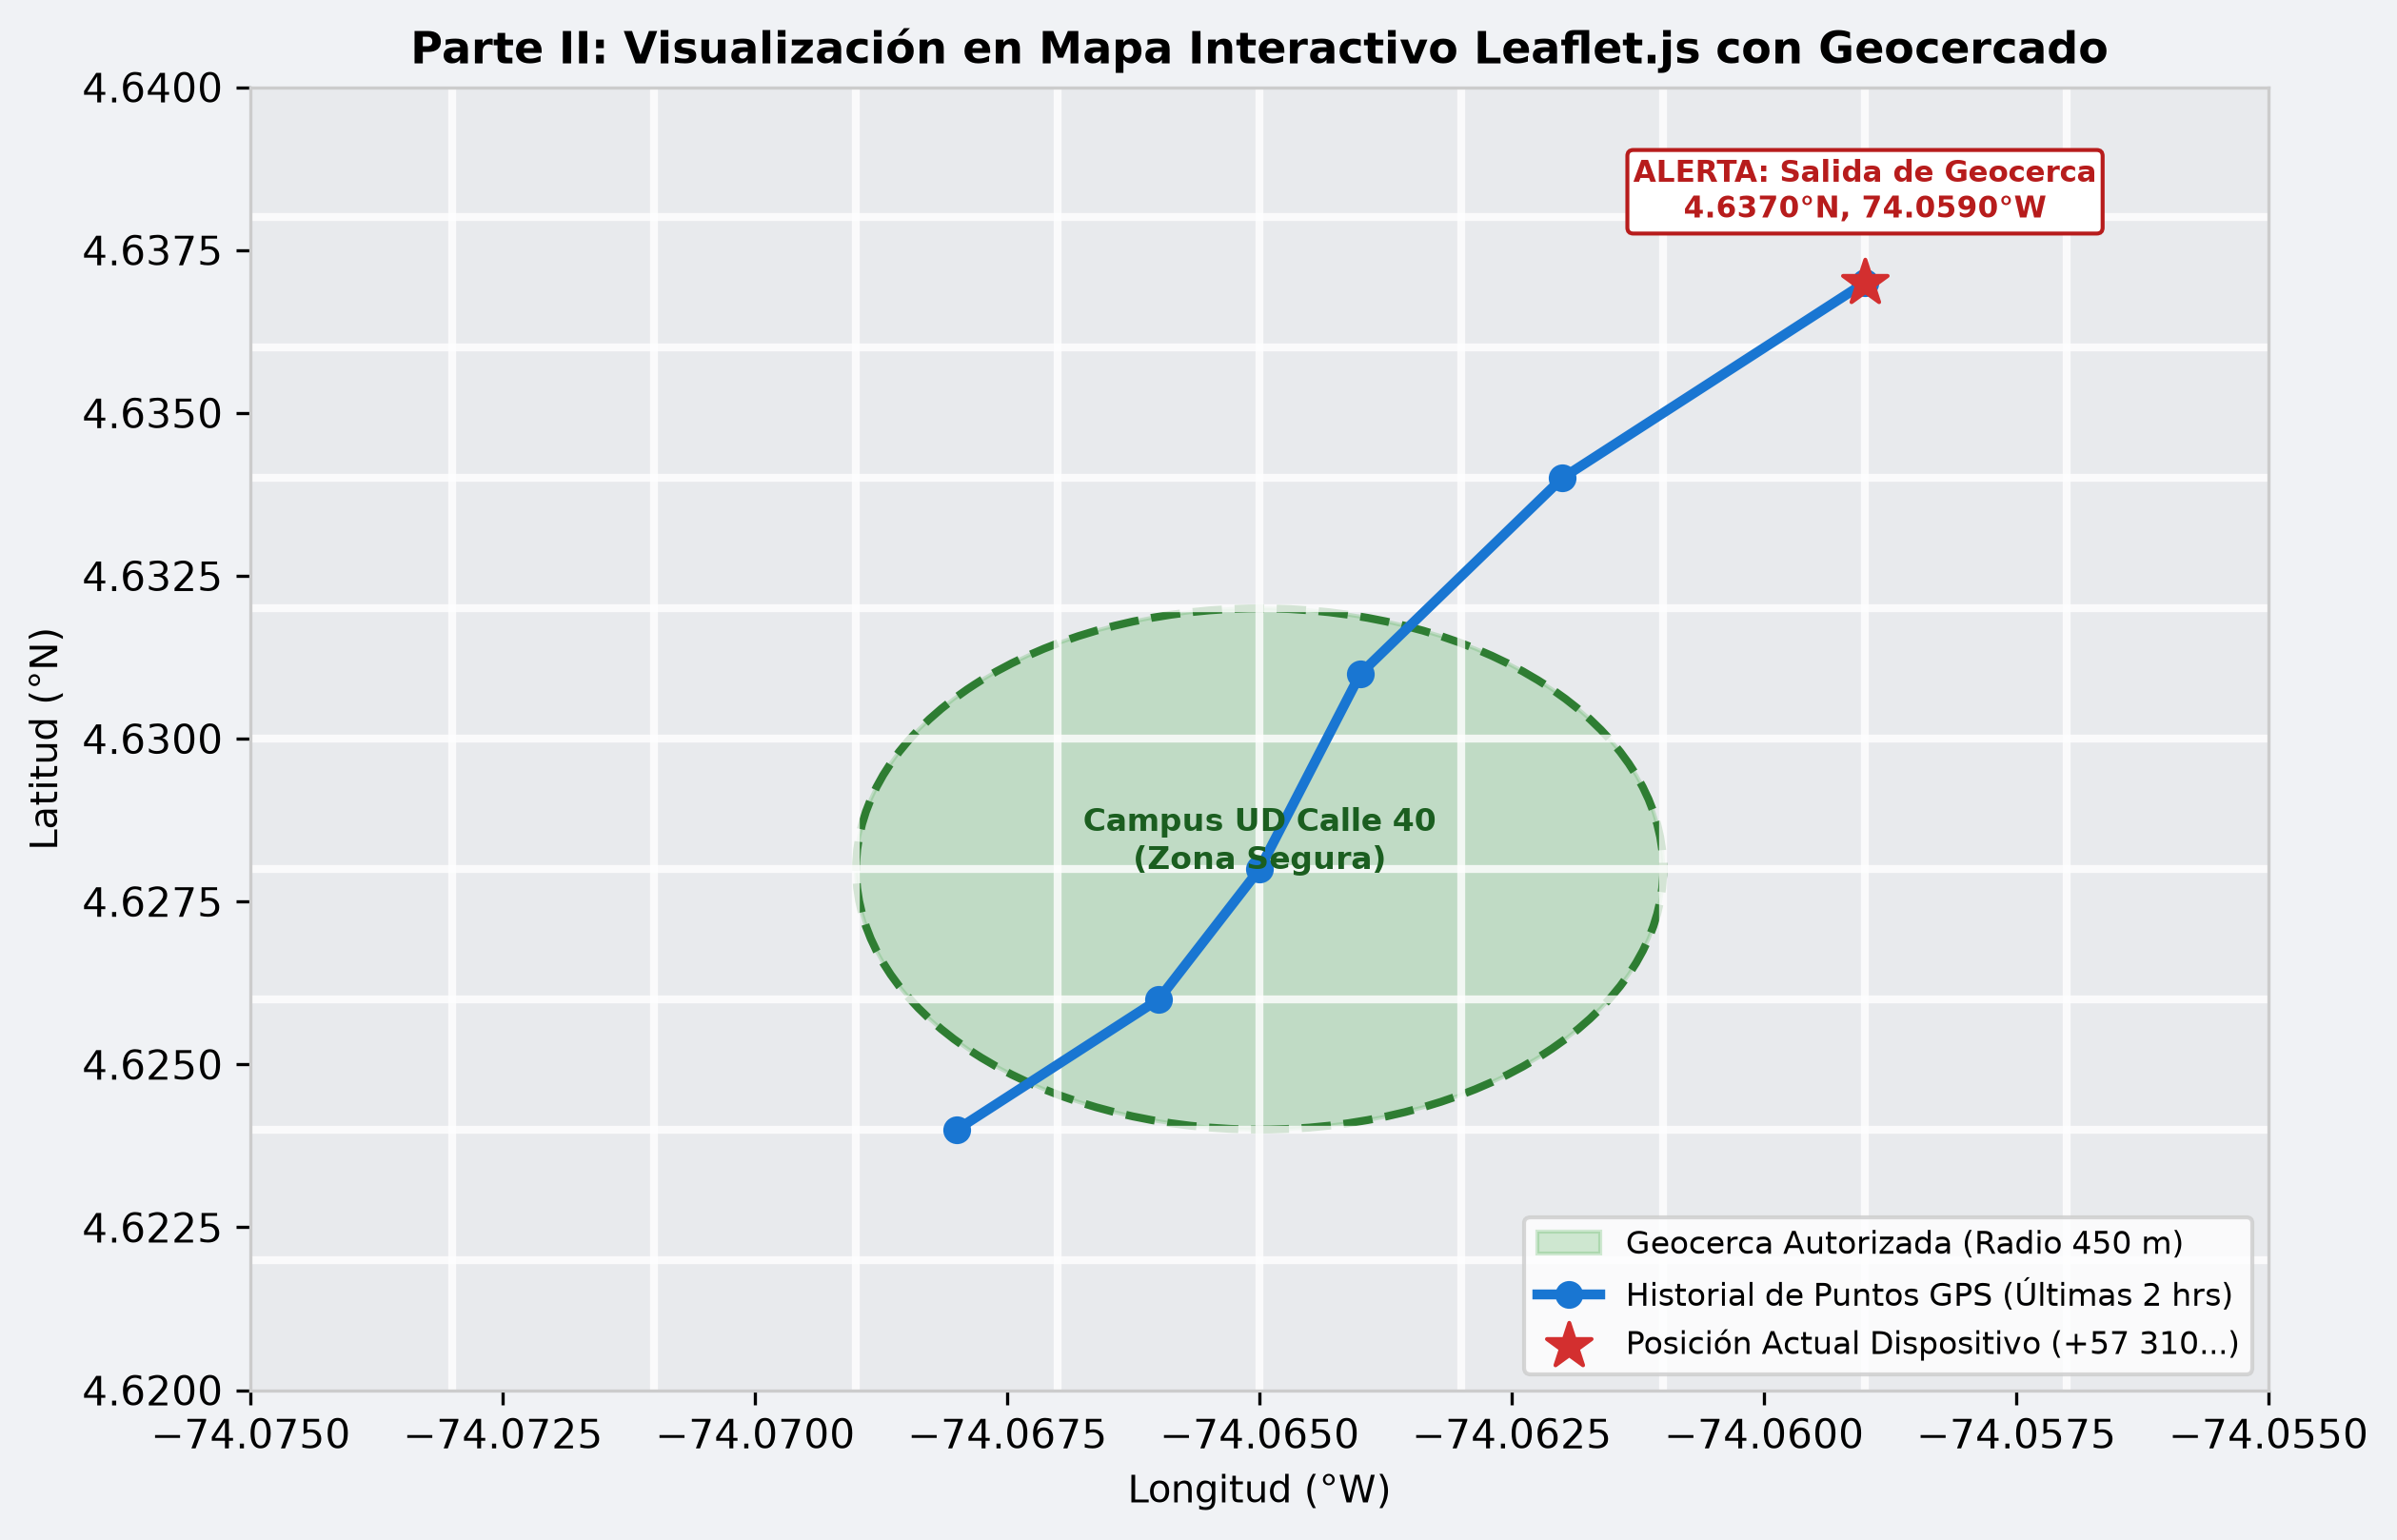
\includegraphics[width=\textwidth]{./images/parte2_mapa_dashboard.png}
        \caption{Mapa Leaflet.js con geocerca en Campus UD y ruta histórica.}
    \end{subfigure}
    \hfill
    \begin{subfigure}[b]{0.45\textwidth}
        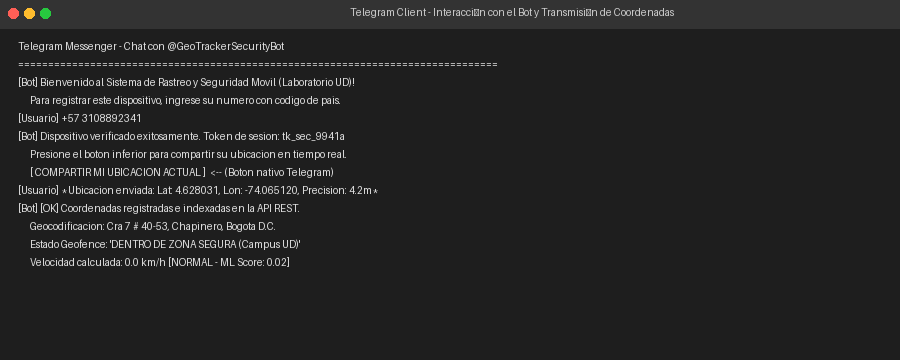
\includegraphics[width=\textwidth]{./images/parte2_telegram_bot.png}
        \caption{Interacción y teclado nativo en el Bot de Telegram.}
    \end{subfigure}
    \caption{Visualización del Dashboard Web y Flujo de Mensajería en Telegram.}
    \label{fig:parte2_dashboard}
\end{figure}

\begin{figure}[H]
    \centering
    \begin{subfigure}[b]{0.50\textwidth}
        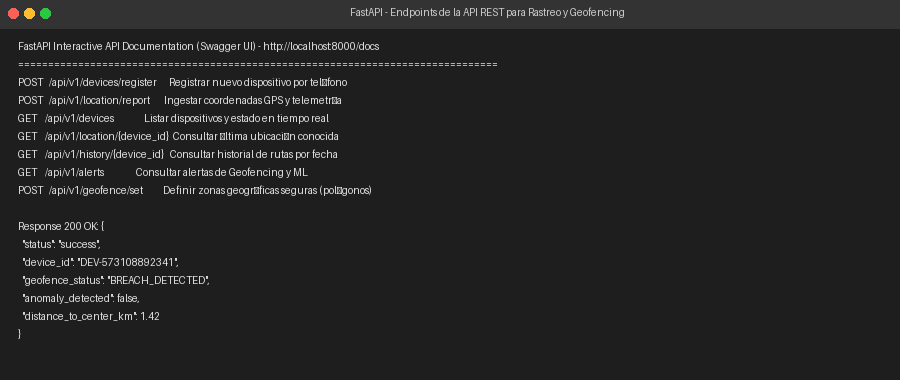
\includegraphics[width=\textwidth]{./images/parte2_swagger_api.png}
        \caption{Documentación interactiva de la API REST (Swagger UI).}
    \end{subfigure}
    \hfill
    \begin{subfigure}[b]{0.48\textwidth}
        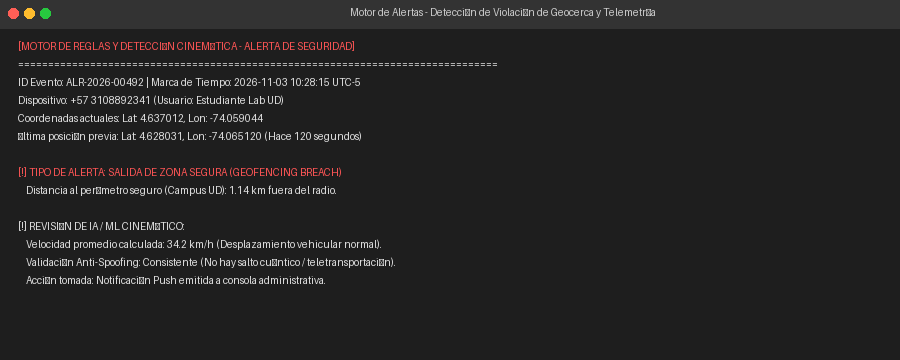
\includegraphics[width=\textwidth]{./images/parte2_geofencing_alert.png}
        \caption{Alerta generada por salida de geocerca y chequeo cinemático.}
    \end{subfigure}
    \caption{Auditoría de Endpoints REST y Disparo de Alertas de Seguridad.}
    \label{fig:parte2_api}
\end{figure}

\subsection{Marco Ético, Jurídico y de Seguridad Informática}
El diseño e implementación de este sistema se realizó bajo el cumplimiento irrestricto de las normativas vigentes en Colombia:

\begin{enumerate}
    \item \textbf{Ley Estatutaria 1581 de 2012 (Habeas Data):} Los datos de geolocalización constituyen datos personales sensibles. El sistema implementa:
    \begin{itemize}
        \item \textbf{Consentimiento Previo, Expreso e Informado:} El usuario debe autorizar de manera inequívoca la captura de telemetría mediante checkbox digital y activación voluntaria en Telegram.
        \item \textbf{Finalidad Legítima y Proporcionalidad:} Los datos se recolectan exclusivamente con fines académicos y de seguridad perimetral.
        \item \textbf{Derecho de Supresión:} Endpoints dedicados para revocar el consentimiento y purgar el historial de ubicaciones almacenado.
    \end{itemize}
    \item \textbf{Ley 1273 de 2009 (Delitos Informáticos en el Código Penal):} Queda terminantemente prohibido el uso de técnicas de interceptación, clonación de SIM (SIM Swapping) o acceso abusivo a sistemas informáticos (Art. 269A y 269F). El sistema opera como software de rastreo consentido, no como herramienta de espionaje o ataque.
    \item \textbf{Seguridad de Datos:} Toda la comunicación se transfiere bajo túneles TLS 1.3 con certificados válidos y los tokens de acceso son generados con algoritmos pseudoaleatorios criptográficamente seguros (\texttt{secrets.token\_hex}).
\end{enumerate}

\newpage
% ==============================================================================
% SECCIÓN 4: CONCLUSIONES Y PLAN DE MEJORA
% ==============================================================================
\section{Conclusiones, Límites de la Evidencia y Plan de Mejora}

\subsection{Conclusiones Técnicas}
\begin{enumerate}
    \item La defensa efectiva de redes Ethernet IEEE 802.3 y servidores TCP/IP exige una estrategia en profundidad: los controles perimetrales (firewalls de estado) resultan insuficientes ante ataques sofisticados como canales encubiertos DNS/ICMP o inyecciones de control TCP RST, requiriendo inspección profunda de paquetes (DPI), análisis de entropía y endurecimiento de protocolos (RFC 5961, DNS RPZ).
    \item La Inteligencia Artificial y el Machine Learning aportan un valor excepcional en la detección temprana de anomalías no firmadas y en el triage asistido de alertas en centros SOC. Sin embargo, su despliegue debe mantener de manera innegociable el principio de \textit{Human-in-the-Loop}, evitando la automatización de bloqueos disruptivos de infraestructura basados únicamente en puntuaciones probabilísticas para prevenir la auto-denegación de servicio.
    \item En sistemas de geolocalización y monitoreo de terminales móviles, la viabilidad técnica está indisolublemente vinculada al marco legal y ético: no existen mecanismos viables de rastreo silencioso mediante servicios como WhatsApp o Telegram sin el concurso activo y el consentimiento explícito del titular, garantizando el respeto al derecho fundamental de Habeas Data.
\end{enumerate}

\subsection{Límites Epistemológicos de la Evidencia Digital}
\begin{itemize}
    \item \textbf{Falibilidad de la Dirección IP:} Una dirección IP observada en un encabezado jamás debe considerarse como prueba incontrovertible de autoría. El IP spoofing en protocolos no orientados a conexión (UDP, ICMP) y el uso de técnicas de rebote o señuelos en TCP impiden la atribución perentoria sin correlación con registros de capa de enlace (MAC, tablas CAM de switches y bitácoras DHCP/RADIUS).
    \item \textbf{Sesgo y Deriva en Modelos de Detección:} Los modelos de aprendizaje automático son vulnerables a la deriva de concepto (\textit{Concept Drift}) y a cambios operacionales benignos, requiriendo auditoría continua de precisión y recall sobre conjuntos de datos actualizados.
\end{itemize}

\subsection{Plan de Mejora Priorizado para la Infraestructura}
\begin{table}[H]
    \centering
    \small
    \begin{tabular}{@{}llll@{}}
        \toprule
        \textbf{Horizonte} & \textbf{Medida de Seguridad Propuesta} & \textbf{Impacto Esperado} & \textbf{Responsable} \\
        \midrule
        \textbf{Corto Plazo} & Desactivar servicios en claro (Telnet, FTP) y habilitar & Eliminación de vectores de robo de & Admin Servidor \\
        (1 a 3 semanas) & SYN Cookies (\texttt{net.ipv4.tcp\_syncookies = 1}) & credenciales e indisponibilidad DoS & \\
        \midrule
        \textbf{Mediano Plazo} & Implementar filtrado BCP 38 (uRPF) en gateways y & Mitigación de amplificación UDP y & Admin Redes \\
        (1 a 2 meses) & desplegar DNS RPZ para bloqueo de dominios anómalos & contención de canales encubiertos & y Telecomunicaciones \\
        \midrule
        \textbf{Largo Plazo} & Despliegue de plataforma SIEM con correlación IA & Detección unificada de incidentes & Equipo de \\
        (3 a 6 meses) & explicable y migración a arquitectura Zero Trust & y reducción de fatiga de alertas SOC & Ciberseguridad / SOC \\
        \bottomrule
    \end{tabular}
    \caption{Plan de Mejora Priorizado para la Infraestructura de Servidores y Redes.}
\end{table}

\newpage
% ==============================================================================
% REFERENCIAS BIBLIOGRÁFICAS
% ==============================================================================
\begin{thebibliography}{99}
    \bibitem{salcedo2026} Salcedo Parra, O. J. (2026). \textit{Fundamentos de Redes de Comunicaciones y Mecanismos de Seguridad Informática: Guía-Taller No. 2}. Universidad Distrital Francisco José de Caldas, Facultad de Ingeniería.
    \bibitem{rfc5961} Ramaiah, A., Stewart, R., \& Dalal, M. (2010). \textit{Improving TCP's Robustness to Blind In-Window Attacks}. RFC 5961, Internet Engineering Task Force (IETF).
    \bibitem{bcp38} Ferguson, P., \& Senie, D. (2000). \textit{Network Ingress Filtering: Defeating Denial of Service Attacks which employ IP Source Address Spoofing}. BCP 38 / RFC 2827, IETF.
    \bibitem{kurose2021} Kurose, J. F., \& Ross, K. W. (2021). \textit{Computer Networking: A Top-Down Approach} (8th ed.). Pearson.
    \bibitem{stallings2020} Stallings, W. (2020). \textit{Cryptography and Network Security: Principles and Practice} (8th ed.). Pearson.
    \bibitem{scikit2024} Pedregosa, F., et al. (2011). \textit{Scikit-learn: Machine Learning in Python}. Journal of Machine Learning Research, 12, 2825-2830.
    \bibitem{ley1581} Congreso de la República de Colombia. (2012). \textit{Ley Estatutaria 1581 de 2012: Por la cual se dictan disposiciones generales para la protección de datos personales (Habeas Data)}. Diario Oficial No. 48.587.
    \bibitem{ley1273} Congreso de la República de Colombia. (2009). \textit{Ley 1273 de 2009: Por medio de la cual se crea y se protege la información y los datos y se preservan integralmente los sistemas que utilicen las tecnologías de la información y las comunicaciones}. Diario Oficial No. 47.223.
\end{thebibliography}

\end{document}
